\documentclass[a4paper, 12pt]{report}

\usepackage[dvipsnames]{xcolor}

%%%%%%%%%%%%%%%%
% Set Variables %
%%%%%%%%%%%%%%%%

\def\useItalian{0}  % 1 = Italian, 0 = English

\def\courseName{Graph Theory}

\def\coursePrerequisites{\begin{itemize} \item Progettazione degli Algoritmi \end{itemize}}

% \def\book{TODO}

% \def\authorName{Simone Bianco}
% \def\email{bianco.simone@outlook.it}
% \def\github{https://github.com/Exyss/university-notes}
% \def\linkedin{https://www.linkedin.com/in/simone-bianco}

\def\authorName{Alessio Bandiera}
\def\email{alessio.bandiera02@gmail.com}
\def\github{https://github.com/aflaag-notes}
\def\linkedin{https://www.linkedin.com/in/alessio-bandiera-a53767223}

%%%%%%%%%%%%
% Packages %
%%%%%%%%%%%%

\usepackage{../../packages/Nyx/nyx-packages}
\usepackage{../../packages/Nyx/nyx-styles}
\usepackage{../../packages/Nyx/nyx-frames}
\usepackage{../../packages/Nyx/nyx-macros}
\usepackage{../../packages/Nyx/nyx-title}
\usepackage{../../packages/Nyx/nyx-intro}

%%%%%%%%%%%%%%
% Title-page %
%%%%%%%%%%%%%%

\logo{../../packages/Nyx/logo.png}

\if\useItalian1
    \institute{\curlyquotes{\hspace{0.25mm}Sapienza} Università di Roma}
    \faculty{Ingegneria dell'Informazione,\\Informatica e Statistica}
    \department{Dipartimento di Informatica}
    \ifdefined\book
        \subtitle{Appunti integrati con il libro \book}
    \fi
    \author{\textit{Autore}\\\authorName}
\else
    \institute{\curlyquotes{\hspace{0.25mm}Sapienza} University of Rome}
    \faculty{Faculty of Information Engineering,\\Informatics and Statistics}
    \department{Department of Computer Science}
    \ifdefined\book
        \subtitle{Lecture notes integrated with the book \book}
    \fi
    \author{\textit{Author}\\\authorName}
\fi


\title{\courseName}
\date{\today}

% \supervisor{Linus \textsc{Torvalds}}
% \context{Well, I was bored\ldots}

\addbibresource{./references.bib}

%%%%%%%%%%%%
% Document %
%%%%%%%%%%%%

\begin{document}
    \maketitle

    % The following style changes are valid only inside this scope 
    {
        \hypersetup{allcolors=black}
        \fancypagestyle{plain}{%
        \fancyhead{}        % clear all header fields
        \fancyfoot{}        % clear all header fields
        \fancyfoot[C]{\thepage}
        \renewcommand{\headrulewidth}{0pt}
        \renewcommand{\footrulewidth}{0pt}}

        \romantableofcontents
    }

    \introduction

    %%%%%%%%%%%%%%%%%%%%%

    \chapter{Basics of Graph Theory}

    In the 18th century, in the city of \href{https://en.wikipedia.org/wiki/K%C3%B6nigsberg}{Königsberg} (Prussia), a puzzle captured the imagination of the townspeople. Königsberg, nestled along the winding \tit{Pregel River}, was divided into four land masses --- two parts of the mainland and two islands, Kneiphof and Lomse. Connecting these regions were \tbf{seven bridges}, crisscrossing the river back and forth.

    Over time, a curious question arose among the people of Königsberg: was it possible to take a \tit{walk} through the city, crossing each of the seven bridges \tbf{exactly once}, without retracing any steps, and ending the walk in the same place where it started? This is known as the \href{https://en.wikipedia.org/wiki/Seven_Bridges_of_K%C3%B6nigsberg}{Seven Bridges of Königsberg} problem.

        It seemed simple enough, yet no one had managed to do it. The challenge became a favorite pastime, debated in marketplaces and whispered about in taverns. Some claimed it was possible with the right path, while others remained skeptical.

    \centeredimage[The map of Königsberg in Euler's time, showing the actual layout of the seven bridges \cite{bridges}.]{0.5}{../assets/konigsberg.png}

    Word of this peculiar problem reached the brilliant Swiss mathematician \href{/}{Leonhard Euler}, a man whose mind was always drawn to patterns and logic. Intrigued, Euler set out to solve the riddle --- not by drawing endless maps or walking the streets himself, but by \tbf{abstracting} the problem into something entirely new.

    Euler realized that the specific layout of the city was \tit{irrelevant}. What truly mattered was the way the landmasses were connected by the bridges. He represented each landmass as a \tbf{dot} and each bridge as a \tbf{line} between them. In doing so, he stripped away unnecessary details and created a simple, elegant combinatorial structure that we now refer to as \tbf{graph}.

    \begin{figure}[H]
        \centering
        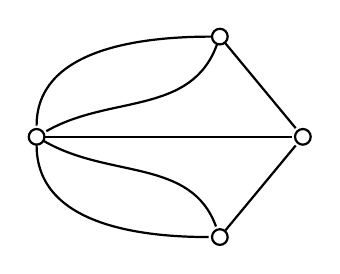
\begin{tikzpicture}[-,>=stealth,shorten >=1pt,auto,node distance=3cm,thick,main node/.style={scale=0.6,circle,draw,font=\sffamily\normalsize}]
            \node[main node] (1) {};
            \node[main node] (2) [below left of=1, xshift = -50] {};
            \node[main node] (3) [below right of=2, xshift = 50] {};
            \node[main node] (4) [right of=2, xshift = 75] {};

            \path[every node/.style={font=\sffamily\small}]
                (1) edge [out=180, in=90] (2)
                (1) edge [out=-110, in=30] (2)
                (2) edge [out=270, in=180] (3)
                (2) edge [out=-30, in=110] (3)
                (2) edge (4)
                (1) edge (4)
                (3) edge (4)
                ;
        \end{tikzpicture}
        \caption{The graph drawn by Euler which models the \tit{Seven Bridges of Königsberg} problem.}
        \label{konigsberg}
    \end{figure}

    Through his analysis, Euler discovered a fundamental rule: for a walk to cross each bridge exactly once and return to the starting point, every landmass had to be connected by an \tbf{even} number of bridges. In Königsberg's case, however, each landmass had an odd number of bridges, making the task impossible.

    Euler's proof, published in 1736, was groundbreaking --- not just because he solved the Königsberg puzzle, but because he laid the foundation for an entirely new branch of mathematics: \href{https://en.wikipedia.org/wiki/Graph_theory}{graph theory}. His ideas would go on to shape the study of networks, from modern transportation systems to social media connections and even the vast web of the internet itself. And so, from a simple question about bridges in a small Prussian city, a whole new field of mathematics was born --- one that continues to shape the world centuries later.

    This chapter will discuss the basics of the field of \tbf{graph theory}, and will lay the foundation for later chapters.

    \section{Introduction}

    \begin{frameddefn}{Graph}
        A \tbf{graph} is a pair $G = (V, E)$, where $V$ is the --- finite --- set of \tbf{vertices} of the graph, and $E$ is the set of \tbf{edges}.
    \end{frameddefn}

    For now, will assume to be working with \tbf{simple} and \tbf{undirected} graphs, i.e. graphs in which the set of edges is defined as follows $$E \subseteq [V]^2 = \{\{x, y\} \mid x, y \in V \land x \neq v\}$$ where the notation $\{x, y\}$ will be used to indicate an edge between two nodes $x, y \in V$, and will be replaced with $xy = yx$ directly --- the \tit{set} notation for edges is used to highlight that edges have no direction.

    We will indicate with $n$ and $m$ the cardinality of $\abs V$ and $\abs E$, respectively. Moreover, we will indicate with $V(G)$ and $E(G)$ the set of the vertices and edges of $G$ respectively when there is ambiguity.

    \begin{figure}[H]
        \centering
        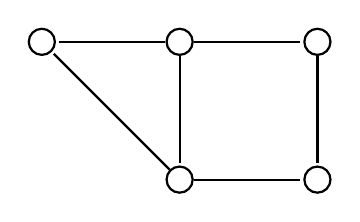
\begin{tikzpicture}[-,>=stealth,shorten >=1pt,auto,node distance=1.75cm, thick,main node/.style={scale=0.9,circle,draw,font=\sffamily\normalsize}]

            \node[circle, draw] (1) []{};
            \node[circle, draw] (2) [right of = 1]{};
            \node[circle, draw] (3) [below of = 1]{};
            \node[circle, draw] (4) [below of = 2]{};
            \node[circle, draw] (5) [left of = 1]{};

            \draw[-] (1) to (2);
            \draw[-] (1) to (3);
            \draw[-] (2) to (4);
            \draw[-] (1) to (5);
            \draw[-] (3) to (4);
            \draw[-] (3) to (5);

            ;
        \end{tikzpicture}
        \caption{A simple graph.}
        \label{first graph}
    \end{figure}

    Note that, in this definition, we are assuming that each edge has exactly 2 \tit{distinct} endpoints --- i.e. the graphs do not admit \tbf{loops} --- and there cannot be two edges with the same endpoints --- i.e. the graphs do not admit \tbf{parallel edges}. In fact, if we drop these assumptions, we obtain what is called a \tbf{multigraph}.

    \begin{figure}[H]
        \centering
        \begin{tikzpicture}[-,>=stealth',shorten >=1pt,auto,node distance=3cm,thick,main node/.style={scale=0.6,circle,draw,font=\sffamily\normalsize},every loop/.style={}]
            \node[main node] (1) {};
            \node[main node] (2) [below left of=1] {};
            \node[main node] (3) [below right of=2] {};

            \draw[-] (1) edge [bend left] (2);
            \draw[-] (1) edge [bend right](2);
            \draw[-] (2) edge (3);
            \draw[-] (3) edge (1);
            \draw[-] (3) edge [loop below] (3);

            ;
        \end{tikzpicture}
        \caption{A multigraph.}
    \end{figure}

    \begin{frameddefn}{Subgraph}
        Given a graph $G = (V, E)$, a \tbf{subgraph} $G' = (V', E')$ of $G$ is a graph such that $V' \subseteq V$ and $E' \subseteq E$, and we write $G' \subseteq G$. If $G'$ is a subgraph of $G$, then $G$ is called \tbf{supergraph} of $G'$.
    \end{frameddefn}

    \begin{figure}[H]
        \centering
        \begin{tikzpicture}[-,>=stealth,shorten >=1pt,auto,node distance=1.75cm, thick,main node/.style={scale=0.9,circle,draw,font=\sffamily\normalsize}]

            \node[circle, draw] (1) []{};
            \node[circle, draw] (2) [right of = 1]{};
            % \node[circle, draw] (3) [below of = 1]{};
            \node[circle, draw] (4) [below of = 2]{};
            \node[circle, draw] (5) [left of = 1]{};

            % \draw[-] (1) to (2);
            % \draw[-] (1) to (3);
            % \draw[-] (2) to (4);
            \draw[-] (1) to (5);
            % \draw[-] (3) to (4);
            % \draw[-] (3) to (5);

            ;
        \end{tikzpicture}
        \caption{This is a subgraph of the graph shown in \cref{first graph}.}
    \end{figure}

    \begin{frameddefn}{Induced subgraph}
        Given a graph $G = (V, E)$, and a set of vertices $S \subseteq V$, then $G[S]$ represents the \tbf{subgraph induced by $S$ on $G$}, obtained by removing from $G$ all the nodes of $V - S$ and the edges incident on them.
    \end{frameddefn}

    In other words, a subgraph $G' = (V', E')$ of $G$ is \tbf{induced} if every edge of $G$ with both ends in $V$ is an edge of $V'$. We observe that this definition is \tit{stricter} than the definition of a \tit{subgraph}; in fact, the last graph is \tit{not} an example of an \tit{induced subgraph}, but the following is:

    \begin{figure}[H]
        \centering
        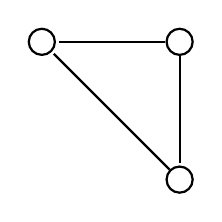
\begin{tikzpicture}[-,>=stealth,shorten >=1pt,auto,node distance=1.75cm, thick,main node/.style={scale=0.9,circle,draw,font=\sffamily\normalsize}]

            \node[circle, draw] (1) []{};
            % \node[circle, draw] (2) [right of = 1]{};
            \node[circle, draw] (3) [below of = 1]{};
            % \node[circle, draw] (4) [below of = 2]{};
            \node[circle, draw] (5) [left of = 1]{};

            % \draw[-] (1) to (2);
            \draw[-] (1) to (3);
            % \draw[-] (2) to (4);
            \draw[-] (1) to (5);
            % \draw[-] (3) to (4);
            \draw[-] (3) to (5);

            ;
        \end{tikzpicture}
        \caption{This is an \tit{induced} subgraph of the graph shown in \cref{first graph}.}
        \label{induced subgraph first graph}
    \end{figure}

    Note that every induced subgraph of a graph is \tbf{unique} by definition, and we indicate each induced subgraph as follows: suppose that the graph in \cref{first graph} had the following \tit{labeling} on the vertices

    \begin{figure}[H]
        \centering
        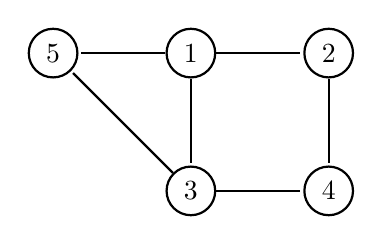
\begin{tikzpicture}[-,>=stealth,shorten >=1pt,auto,node distance=1.75cm, thick,main node/.style={scale=0.9,circle,draw,font=\sffamily\normalsize}]

            \node[circle, draw] (1) []{1};
            \node[circle, draw] (2) [right of = 1]{2};
            \node[circle, draw] (3) [below of = 1]{3};
            \node[circle, draw] (4) [below of = 2]{4};
            \node[circle, draw] (5) [left of = 1]{5};

            \draw[-] (1) to (2);
            \draw[-] (1) to (3);
            \draw[-] (2) to (4);
            \draw[-] (1) to (5);
            \draw[-] (3) to (4);
            \draw[-] (3) to (5);

            ;
        \end{tikzpicture}
        % \caption{This is an \tit{induced} subgraph of the graph shown in \cref{first graph}.}
    \end{figure}

    then, the induced subgraph in \cref{induced subgraph first graph} would have been referred to as $G[\{1, 3, 5\}]$. To clarify, when writing $G - A$

    \begin{itemize}
        \item if $A$ is a set of \tit{vertices} we are referring to $G[V(G) - A]$ --- a vertex cannot be removed from a graph without removing all the edges incident to it
        \item if $A$ is a set of \tit{edges} we are refering to a graph $G$ without the edges in $A$ --- note that this graph has still $V(G)$ as vertex set
    \end{itemize}

    \begin{frameddefn}{Graph union}
        Given two graphs $G$ and $G'$, we define the \tbf{union} $G \cup G'$ as the following graph:

        \begin{itemize}
            \item $V(G \cup G') := V(G) \cup V(G')$
            \item $E(G \cup G') := E(G) \cup E(G')$ 
        \end{itemize}
    \end{frameddefn}

    Intuitively, two vertices $x, y \in V$ are said to be \tbf{adjacent} if there is an edge $xy \in E$, and we write $x \sim y$. If there is no such edge, we write $x \nsim y$ for non-adjacency and we say that $xy$ is an \tbf{anti-edge}. The \tbf{neighborhood} of a vertex $x \in V$ is the set of vertices that are adjacent to $x$, and it will be indicated as follows $$\mathcal N (x) := \{y \in V \mid x \sim y\}$$ Similarly, the neighborhood of a set of vertices will be defined as follows $$\forall S \subseteq V \quad \mathcal N(S) := \bigcup_{v \in S}{\mathcal N (v)}$$ The \tbf{degree} of a vertex $x \in V$, denoted with $\deg(x)$, is exactly $\abs{\mathcal N (x)}$. We will use the following notation for the \tbf{minimum} and \tbf{maximum} degree of a graph, respectively

    \begin{center}
        \begin{tabular}{ccc}
            $\displaystyle \delta := \min_{x \in V}{\deg(x)}$ & \qquad & $\displaystyle \Delta := \max_{x \in V}{\deg(x)}$
        \end{tabular}
    \end{center}

    \begin{framedlem}{Handshaking lemma}
        Given a graph $G = (V, E)$, it holds that $$\sum_{x \in V}{\deg(x)} = 2 \abs E$$
    \end{framedlem}

    \begin{proof}
        Trivially, the sum of the degrees counts every edge in $E$ exactly twice, once for each of the 2 endpoints.
    \end{proof}

    \begin{framedcor}[label={cor handshaking}]{}
        Given a graph $G = (V, E)$, it holds that $\abs{E} \ge \tfrac{\delta \cdot n}{2}$.
    \end{framedcor}

    \begin{proof}
        By the Handshaking lemma, we have that $$2 \abs E = \sum_{x \in V}{\deg(x)} \ge \delta \cdot n \iff \abs E \ge \dfrac{\delta \cdot n}{2}$$
    \end{proof}

    \begin{frameddefn}{$k$-regular graph}
        A graph $G$ is said to be \tbf{$k$-regular} if every vertex of $G$ has degree $k$.
    \end{frameddefn}

    Note that in a $k$-regular graph it holds that $$\sum_{x \in V}{\deg(x)} = k \cdot n$$

    \begin{framedprop}{}
        There are no $k$-regular graphs with $k$ odd and an odd number of vertices.
    \end{framedprop}
    
    \begin{proof}
        By way of contradiction, suppose that there exists a $k$-regular graph $G = (V, E)$ such that both $k$ and $n$ are odd; however, by the Handshaking lemma we would get that $$2 \abs E = \sum_{x \in V} {\deg(x)} = k \cdot n$$ but the product of two odd numbers, namely $k$ and $n$, is still an odd number, while $2 \abs E$ must be even $\lightning$.
    \end{proof}

    \section{Important structures}

    \begin{frameddefn}{Path}
        A \tbf{path} is a \tit{graph} with vertex set $x_0, \ldots, x_n$ and edge set $e_1, \ldots, e_n$ such that $e_i = x_{i - 1}x_i$.

        The \tbf{length} of a path is the number of edges between $x_0$ and $x_n$, i.e. $\abs{\{e_1, \ldots, e_n\}}$, namely $n$ in this case. A path of length 1 is called \tit{trivial} path. $P_n$ is the path graph having $n$ vertices.
    \end{frameddefn}

    \begin{figure}[H]
        \centering
        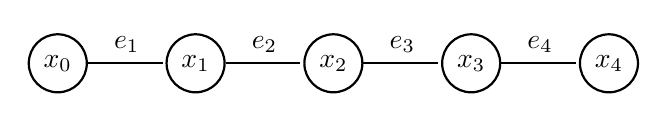
\begin{tikzpicture}[-,>=stealth,shorten >=1pt,auto,node distance=1.75cm, thick,main node/.style={scale=0.9,circle,draw,font=\sffamily\normalsize}]

            \node[circle, draw] (1) []{$x_0$};
            \node[circle, draw] (2) [right of = 1]{$x_1$};
            \node[circle, draw] (3) [right of = 2]{$x_2$};
            \node[circle, draw] (4) [right of = 3]{$x_3$};
            \node[circle, draw] (5) [right of = 4]{$x_4$};

            \draw[-] (1) to node[above]{$e_1$} (2);
            \draw[-] (2) to node[above]{$e_2$} (3);
            \draw[-] (3) to node[above]{$e_3$} (4);
            \draw[-] (4) to node[above]{$e_4$} (5);

            ;
        \end{tikzpicture}
        \caption{A path graph of length 4 that links $x_0$ and $x_4$.}
    \end{figure}

    Through \tit{paths} we can provide the definition of \tbf{distance} between two nodes of a graph.

    \begin{frameddefn}{Distance}
        Given a graph $G = (V, E)$, and two vertices $x, y \in V$, the \tbf{distance} between $x$ and $y$ in $G$, denoted with $\dist_G(x, y)$, is defined as the length of the \tit{shortest} path between $x$ and $y$ in $G$.
    \end{frameddefn}

    If there is no ambiguity, we will simply write $\dist(x, y)$ instead of $\dist_G(x, y)$. Finally, given a path $P$ and two vertices $u, v \in V(P)$, we will denote with $u \ P \ v$ the \tit{subpath} of $P$ between $u$ and $v$. Now, consider the following definition.

    \begin{frameddefn}{Walk}
        Given a graph $G = (V, E)$, a \tbf{walk} is a \tit{sequence} of vertices and edges $$x_0 \ e_1 \ x_1 \ \ldots \ x_{k - 1} \ e_k \ x_k$$ where $x_0, \ldots, x_k \in V$, $e_1, \ldots, e_k \in E$ and $e_i = x_{i - 1}x_i$.

        The \tbf{length} of a walk is the number of edges between $x_0$ and $x_k$, i.e. $\abs{\{e_1, \ldots , e_k \}}$, namely $k$ in this case. If $x_0 = x_k$ we say that the walk is \tbf{closed}.
    \end{frameddefn}

    If there is a path -- or a walk --- between two vertices $x, y \in V$, we say that the path --- or the walk --- \tbf{links} $x$ and $y$, and we write this as $x \to y$. Any vertex that is different from $x$ and $y$ is called \tit{internal node}. For instance, given the previous graph labeled as follows

    \begin{figure}[H]
        \centering
        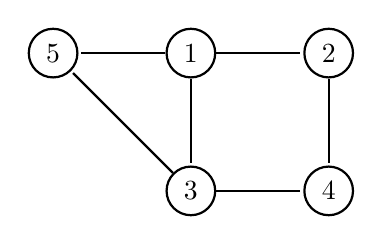
\begin{tikzpicture}[-,>=stealth,shorten >=1pt,auto,node distance=1.75cm, thick,main node/.style={scale=0.9,circle,draw,font=\sffamily\normalsize}]

            \node[circle, draw] (1) []{1};
            \node[circle, draw] (2) [right of = 1]{2};
            \node[circle, draw] (3) [below of = 1]{3};
            \node[circle, draw] (4) [below of = 2]{4};
            \node[circle, draw] (5) [left of = 1]{5};

            \draw[-] (1) to (2);
            \draw[-] (1) to (3);
            \draw[-] (2) to (4);
            \draw[-] (1) to (5);
            \draw[-] (3) to (4);
            \draw[-] (3) to (5);

            ;
        \end{tikzpicture}
        % \caption{Giv}
    \end{figure}

    an example of a walk over this graph is given by the following sequence $$1 \ \{1, 2\} \ 2 \ \{2, 4\} \ 4 \ \{4, 3\} \ 3 \ \{3, 1\} \ 1 \ \{1, 5\} \ 5$$ that \tit{links} 1 and 5, i.e. the walk is of the form $1 \to 5$.

    Note that there is a subtle difference between the definitions of \tbf{path} and \tbf{walk}: the definition of a path implies that this is always a \tit{graph} on its own, while a walk is defined as a \tit{sequence}. Nonetheless, we will treat \tit{paths} as if they where \tit{sequences} as well. This assumption holds for the following structures that will be discussed as well.

    However, by definition of path, not every alternating sequence of vertices and edges is a valid path, in fact:
    
    \begin{itemize}
        \item in a \tit{walk} it is possible to repeat both vertices and edges
        \item in a \tit{path} there can be no repetition of vertices nor edges (note that \tit{edge} repetition implies \tit{vertex} repetition)
    \end{itemize}

    For instance, the previous example of \tit{walk} is not a valid \tit{path}, because the vertex 1 is repeated.

    \begin{framedthm}[label={paths and walks}]{Paths and walks}
        Given a graph $G = (V, E)$ and two vertices $x, y \in V$, in $G$ there is a path $x \to y$ if and only if there is a walk $x \to y$.
    \end{framedthm}

    \begin{proof}
        By definition, every path is a walk, thus the direct implication is trivially true. To prove the converse implication, consider two vertices $x$ and $y$ for which there is at least one walk $x \to y$ in $G$. Now, out of all the possible walks $x \to y$ in $G$, consider the \tit{shortest} one, i.e. the one with the least amount of edges, and let it be the following sequence $$x \ e_1 \ x_1 \ \ldots \ x_{k - 1} \ e_k \ y $$ By way of contradiction, assume that this walk is not a path. Therefore, there must be either one vertex or one edge repeated, but since edge repetition always implies vertex repetition, we just need to take this case into account. Assume that there are two indices $i, j \in [k - 1]$ such that $i \neq j$ and $x_i = x_j$; however this implies that $$x \ e_1 \ \ldots \ x_{i - 1} \ e_i \ x_i \ e_{j + 1} \ x_{j + 1} \ \ldots \ x_{k - 1} \ e_k \ y$$ is still a walk $x \to y$ of strictly shorter length, but we chose the original sequence to be the \tit{shortest} possible walk $x \to y$ $\lightning$.
    \end{proof}

    \begin{framedprop}[label={longest path len}]{}
        The longest path in any graph has a length of at least $\delta$.
    \end{framedprop}
    
    \begin{proof}
        Consider a graph $G = (V, E)$, and let $P$ be a longest path in $G$, labeled as follows $$x_0 \ e_1 \ x_1 \ \ldots \ x_{k - 1} \ e_k \ x_k$$ and assume that its length is $k$. Since $P$ is a longest path in $G$, $x_k$ cannot have neighbors outside $P$ itself, otherwise $P$ would not have been the longest path of $G$ --- it could have been extended by one of $x_k$'s neighbors. This implies that $$\mathcal N(x_k) \subseteq \{x_0, \ldots, x_{k - 1}\}$$ and since $\delta \le \deg(x_k) := \abs{\mathcal N(x_k)}$ by definition of $\delta$, this implies that $$\delta \le \abs{\{x_0, \ldots, x_{k - 1}\}} = k$$
    \end{proof}

    \begin{frameddefn}{Cycle}
        A \tbf{cycle} is a \tit{graph} with vertex set $x_1, \ldots, x_n$ and edge set $x_1x_2, x_2x_3, \ldots, x_{n- 1}x_n, x_nx_1$.

        The \tbf{length} of a cycle is the number of edges between $x_1$ and $x_n$, namely $n$ in this case. $C_n$ is the cycle graph having $n$ vertices.
    \end{frameddefn}

        \begin{figure}[H]
        \centering
        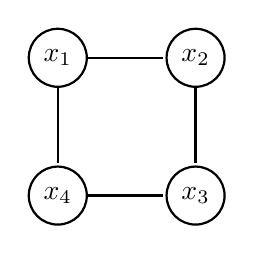
\begin{tikzpicture}[-,>=stealth,shorten >=1pt,auto,node distance=1.75cm, thick,main node/.style={scale=0.9,circle,draw,font=\sffamily\normalsize}]

            \node[circle, draw] (1) []{$x_1$};
            \node[circle, draw] (2) [right of = 1]{$x_2$};
            \node[circle, draw] (3) [below of = 1]{$x_4$};
            \node[circle, draw] (4) [below of = 2]{$x_3$};

            \draw[-] (1) to (2);
            \draw[-] (1) to (3);
            \draw[-] (2) to (4);
            \draw[-] (3) to (4);

            ;
        \end{tikzpicture}
        \caption{A cycle graph of length 4.}
    \end{figure}

    A graph that does not admit cycle subgraphs --- or \tit{cycles}, for short --- is said to be \tbf{acyclic}.

    \begin{framedprop}[label={min deg 2}]{}
        Every graph with $\delta \ge 2$ has a cycle of length at least $\delta + 1$.
    \end{framedprop}

    \begin{proof}
        Consider the proof of \cref{longest path len}; by applying the same reasoning, we know that $x_k$ cannot have neighbors outside $P$ itself. However, since $\delta \ge 2$, and $x_k \sim x_{k - 1}$, there must be at least one vertex in $x_k$'s neighborhood that lies in $P$. Therefore, let $x_i$ be the first vertex of $P$ --- w.r.t. our labeling of $P$ --- that is adjacent to $x_k$; hence, we have $$\mathcal N (x_k) \subseteq \{x_i, \ldots, x_{k - 1}\} \implies \delta \le \abs{\{x_i, \ldots, x_{k - 1}\}}$$ which implies that $x_i, \ldots, x_{k - 1}, x_k, x_i$ is a cycle of length at least $\delta + 1$.
    \end{proof}

    \begin{frameddefn}{Connected graph}
        An undirected graph $G = (V, E)$ is said to be \tbf{connected} if and only if for each vertex pair $x, y \in V$ there is a path $x \to y$.
    \end{frameddefn}

    All the graphs that we presented so far are \tit{connected}, thus the following figure provides an example of an \tbf{disconnected} graph.

    \begin{figure}[H]
        \centering
        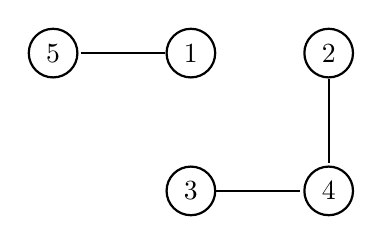
\begin{tikzpicture}[-,>=stealth,shorten >=1pt,auto,node distance=1.75cm, thick,main node/.style={scale=0.9,circle,draw,font=\sffamily\normalsize}]

            \node[circle, draw] (1) []{1};
            \node[circle, draw] (2) [right of = 1]{2};
            \node[circle, draw] (3) [below of = 1]{3};
            \node[circle, draw] (4) [below of = 2]{4};
            \node[circle, draw] (5) [left of = 1]{5};

            % \draw[-] (1) to (2);
            % \draw[-] (1) to (3);
            \draw[-] (2) to (4);
            \draw[-] (1) to (5);
            \draw[-] (3) to (4);
            % \draw[-] (3) to (5);

            ;
        \end{tikzpicture}
        % \caption{An disconnected graph.}
    \end{figure}

    \begin{frameddefn}{Component}
        Given a graph $G$, a \tbf{component} of $G$ is a maximal connected subgraph of $G$.
    \end{frameddefn}

    For instance, the graph of the previous example is made up of 2 components, namely the following two subgraphs $$C_1 = (\{1, 5\}, \{\{1, 5\}\})$$ $$C_2 = (\{2, 3, 4\}, \{\{2, 4\}, \{4, 3\}\})$$

    \begin{framedprop}[label={avoid cycle}]{}
        If $G$ is a connected graph, and $C$ is a cycle in $G$, then for any edge $e \in C$ it holds that $G - \{e\}$ is still connected.
    \end{framedprop}

    \begin{proof}
        Consider a graph $G = (V, E)$ that has a cycle $C$, and any two vertices $x, y \in V$; in particular, since $G$ is connected, there must be a path $x \to y$ in $G$, and let this path be $$P = x \ e_1 \ x_1 \ \ldots \ x_{k - 1} \ e_k \ y$$ Consider an edge $e \in C$; if $P$ does not traverse $e$, trivially $G - \{e\}$ will still contain $P$.

        Now let $$C = z_1 \ f_2 \ z_2 \ \ldots \ z_{l- 1} \ f_l \ z_l \ f_{l + 1} \ z_1$$ and without loss of generality assume that $e = f_2 = z_1 z_2 = x_i x_{i + 1} = e_{i + 1}$ for some $i \in [k - 1]$. Thus we can construct the following walk $$x \ e_1 \ x_1 \ \ldots \ x_i \ f_{l + 1} \ z_l \ \ldots \ f_3 \ z_2 \ e_{i + 2} \ x_{i + 2} \ \ldots \ x_{k - 1} \ e_k \ y$$ from $x$ to $y$, and by \cref{paths and walks} we have that there is a path from $x \to y$, which proves that $G - \{e\}$ is still connected.
    \end{proof}

    \subsection{Trees}

    \begin{frameddefn}{Tree}
        A \tbf{tree} is a connected acyclic graph. Usually, but not necessarily, there is a fixed vertex called \tbf{root}, and any vertex that has degree 1 in the tree is called \tbf{leaf}.
    \end{frameddefn}
    
    \begin{figure}[H]
        \centering
        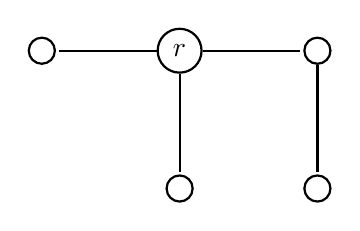
\begin{tikzpicture}[-,>=stealth,shorten >=1pt,auto,node distance=1.75cm, thick,main node/.style={scale=0.9,circle,draw,font=\sffamily\normalsize}]

            \node[circle, draw] (1) []{$r$};
            \node[circle, draw] (2) [right of = 1]{};
            \node[circle, draw] (3) [below of = 1]{};
            \node[circle, draw] (4) [below of = 2]{};
            \node[circle, draw] (5) [left of = 1]{};

            \draw[-] (1) to (2);
            \draw[-] (1) to (3);
            \draw[-] (2) to (4);
            \draw[-] (1) to (5);
            % \draw[-] (3) to (4);
            % \draw[-] (3) to (5);

            ;
        \end{tikzpicture}
        \caption{A tree with tree leaves, rooted in $r$.}
    \end{figure}

    A \tbf{forest} is an disconnected graph in which each component is a \tit{tree}, as in the following example

    \begin{figure}[H]
        \centering
        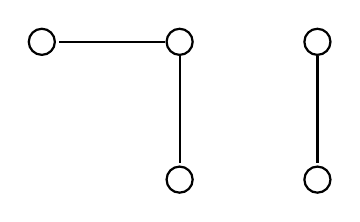
\begin{tikzpicture}[-,>=stealth,shorten >=1pt,auto,node distance=1.75cm, thick,main node/.style={scale=0.9,circle,draw,font=\sffamily\normalsize}]

            \node[circle, draw] (1) []{};
            \node[circle, draw] (2) [right of = 1]{};
            \node[circle, draw] (3) [below of = 1]{};
            \node[circle, draw] (4) [below of = 2]{};
            \node[circle, draw] (5) [left of = 1]{};

            % \draw[-] (1) to (2);
            \draw[-] (1) to (3);
            \draw[-] (2) to (4);
            \draw[-] (1) to (5);
            % \draw[-] (3) to (4);
            % \draw[-] (3) to (5);

            ;
        \end{tikzpicture}
        \caption{A forest.}
    \end{figure}

    Given a tree $T$ rooted in some node $r \in V(T)$, and two vertices $x, y \in V(T)$, consider the paths $P_x$ of the form $x \to r$ and $P_y$ of the form $y \to r$, respectively. The first vertex of $P_y$ that is encountered by tracing $P_x$ from $x$ to $r$ is called \tbf{lowest common ancestor} (LCA) of $x$ and $y$.

    \begin{figure}[H]
        \centering
        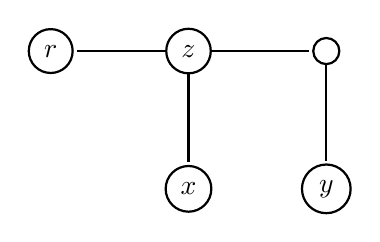
\begin{tikzpicture}[-,>=stealth,shorten >=1pt,auto,node distance=1.75cm, thick,main node/.style={scale=0.9,circle,draw,font=\sffamily\normalsize}]

            \node[circle, draw] (1) []{$z$};
            \node[circle, draw] (2) [right of = 1]{};
            \node[circle, draw] (3) [below of = 1]{$x$};
            \node[circle, draw] (4) [below of = 2]{$y$};
            \node[circle, draw] (5) [left of = 1]{$r$};

            \draw[-] (1) to (2);
            \draw[-] (1) to (3);
            \draw[-] (2) to (4);
            \draw[-] (1) to (5);
            % \draw[-] (3) to (4);
            % \draw[-] (3) to (5);

            ;
        \end{tikzpicture}
        \caption{For instance, in this tree --- rooted in $r$ --- the LCA of $x$ and $y$ is the vertex labeled with $z$.}
    \end{figure}

    Note that the LCA between any two vertices of a tree is \tit{always defined}, since in the \curlyquotes{worst case} it is the root $r$ itself.

    \begin{framedthm}[label={tree alt}]{Alternative definitions of tree}
        Given a graph $T = (V, E)$, the following statements are equivalent:

        \begin{enumerate}
            \item $T$ is a tree
            \item every vertex pair of $T$ is connected by a unique path
            \item $T$ is \tit{minimally connected}, i.e. $T$ is connected and $\forall e \in E$ it holds that $T- \{e\}$ is disconnected
            \item $T$ is \tit{maximally acyclic}, i.e. $T$ is acyclic and $\forall x, y \in V$ such that $x \nsim y$, it holds that $T \cup \{xy\}$ has a cycle
        \end{enumerate}
    \end{framedthm}

    \begin{proof}
        We will prove the statements cyclically.
        \begin{itemize}
            \item $1 \implies 2$. By contrapositive, assume that in $T$ there exist two vertices $x, y \in V$ for which there are two distinct paths $P$ and $Q$ of the form $x \to y$. If $P$ and $Q$ are edge-disjoint, then $P \cup Q$ is a cycle, which implies that $T$ is not a tree by definition.

                Otherwise, assume that $P$ and $Q$ are not edge-disjoint. If we start say in $x$, and we follow $Q$ edge by edge since $P$ and $Q$ are distinct, at some point we will encounter an edge $\{u, v\}$ such that $u \in P \cap Q$ and $v \in Q - P$ --- possibly, $u = x$ itself. Moreover, since both paths lead to $y$, if we keep following $Q$ we will encounter a vertex $z \in P \cap Q$ --- possibly, $z = y$ itself --- from which the two paths will coincide. Let $Q'$ be the subpath of $P$ starting with $u$ and ending in $z$; then, $Q' \cup (Q - P)$ is a cycle in $T$, which implies that $T$ is not a tree by definition.

                \begin{figure}[H]
                    \centering
                    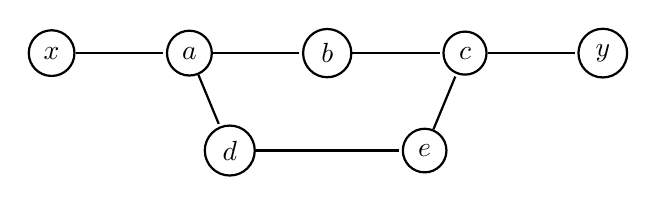
\begin{tikzpicture}[-,>=stealth,shorten >=1pt,auto,node distance=1.75cm, thick,main node/.style={scale=0.9,circle,draw,font=\sffamily\normalsize}]

                        \node[circle, draw] (1) []{$x$};
                        \node[circle, draw] (2) [right of = 1]{$a$};
                        \node[circle, draw] (3) [right of = 2]{$b$};
                        \node[circle, draw] (4) [right of = 3]{$c$};
                        \node[circle, draw] (5) [right of = 4]{$y$};
                        \node[circle, draw] (6) [below left of = 3]{$d$};
                        \node[circle, draw] (7) [below right of = 3]{$e$};

                        \draw[-] (1) to (2);
                        \draw[-] (2) to (3);
                        \draw[-] (3) to (4);
                        \draw[-] (4) to (5);
                        \draw[-] (2) to (6);
                        \draw[-] (7) to (4);
                        \draw[-] (6) to (7);

                        ;
                    \end{tikzpicture}
                    \caption{For instance, applying the argument of the proof in this graph we would get that $P = \{x, a, b, c, y\}$, $Q = \{x, a, d, e, c, y\}$, $Q - P = \{d, e\}$, $u = a$, $z = c$ and $Q' = \{a, b, c\}$, in fact $Q' \cup (Q - P) = \{a, b, c, e, d\}$ which is a cycle.}
                \end{figure}
            \item $2 \implies 3$. Consider an edge $xy \in E$; this edge itself is a path $x \to y$, and if we assume statement 2 this implies that it is the \tit{only} path from $x$ to $y$. This implies that $T - \{xy\}$ cannot contain a path from $x$ to $y$, therefore $T - \{xy\}$ is disconnected.
            \item $3 \implies 4$. Since statement 3 implies that $T$ is connected, by \cref{avoid cycle} we have that $T$ is acyclic. Now, pick $x, y \in V$ such that $x \nsim y$; by connectivity of $T$ there must be a path $x \to y$ in $T$, and let this path be $P$. Lastly, since $x \nsim y$, we have that $P \cup \{xy\}$ is a cycle in $T$.
            \item $4 \implies 1$ By contrapositive, we want to prove that if $T$ is not a tree, then $T$ is not maximally acyclic. Note that if $T$ is not a tree, we have two options:

                \begin{itemize}
                    \item if $T$ is connected but contains a cycle, then $T$ is clearly not maximally acyclic
                    \item if $T$ is acyclic but disconnected, then by definition there must be two vertices $x, y \in V$ such that there is no path $x \to y$, which implies that $T \cup \{xy\}$ still does not contain any cycle
                \end{itemize}
        \end{itemize}
    \end{proof}

    \begin{framedlem}[label={leaf existence}]{}
        Every tree with at least 2 vertices has a leaf.
    \end{framedlem}
    
    \begin{proof}
        By way of contradiction, assume $T$ is a tree with at least 2 vertices that does not contain any leaves; then $\delta \ge 2$ in $T$, which implies that $T$ contains a cycle of length at least $\delta + 1$ by \cref{min deg 2}.
    \end{proof}

    \begin{framedlem}[label={tree without leaf}]{}
        Given a tree $T$, and a leaf $v$ of $T$, it holds that $T - \{v\}$ is still a tree.
    \end{framedlem}

    \begin{proof}
        Since $T$ is acyclic by definition, $T - \{v\}$ is still acyclic, we just need to prove that $T - \{v\}$ is still connected. By way of contradiction, assume that in $T - \{v\}$ there exist two vertices $x$ and $y$ such that there is no path between them. However, since $T$ is connected, there is a path $P$ of the form $x \to y$ in $T$.

        Note that, if by removing $v$ from $T$ we disconnect $x$ and $y$, it must be that $v$ lies in $P$. Moreover, since $v$ is in $T$ but not in $T - \{v\}$, while both $x$ and $y$ are also in $T - \{v\}$, it must be that $v$ is an \tit{internal} node of $P$, i.e. $v \neq x, y$, which implies that $\deg(v) \ge 2$ by definition of path, contradicting the hypothesis for which $v$ was a leaf $\lightning$.
    \end{proof}

    \begin{framedprop}[label={m n - 1}]{}
        If $T$ is a tree, then $m = n - 1$.
    \end{framedprop}

    \proofind{
        We will prove the statement by induction on $n$
    }{
        When $n = 1$, there are no edges in the tree, and $0 = m = 1 - 1$.
    }{
        Assume that for a tree that has $n = k - 1$ nodes the statement holds.
    }{
        We will prove the statement for a tree $T$ that has $n = k$ nodes. Note that, since $n = 1$ is the base case, we can assume that $n = k \ge 2$, hence by \cref{leaf existence} $T$ contains at least one leaf. Let this leaf be $v$; then, by \cref{tree without leaf} it holds that $T - \{v\}$ is still a tree, and clearly $T - \{v\}$ has $k - 1$ nodes, which implies that we can apply the inductive hypothesis on $T - \{v\}$, i.e. $$\abs{E(T - \{v\})} = \abs{V(T - \{v\})} - 1 = k - 1 - 1 = k - 2$$ However, note that $v$ is a leaf, concluding that $$m = \abs{E(T)} = \abs{E(T - \{v\})} + 1 = k - 2 + 1 = k - 1 = n - 1$$
    }

    \begin{frameddefn}{Spanning tree}
        Given a graph $G = (V, E)$, a \tbf{spanning tree} $T$ of $G$ is a subgraph of $G$ such that

        \begin{itemize}
            \item $T$ is a tree
            \item $V(T) = V(G)$, i.e. $T$ \tit{spans} every vertex of $G$
        \end{itemize}
    \end{frameddefn}

    For instance, given the graph in \cref{first graph}, a possible spanning tree is the following:

    \begin{figure}[H]
        \centering
        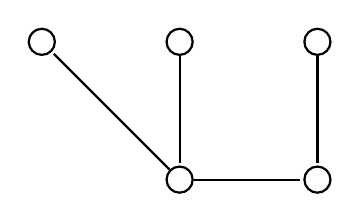
\begin{tikzpicture}[-,>=stealth,shorten >=1pt,auto,node distance=1.75cm, thick,main node/.style={scale=0.9,circle,draw,font=\sffamily\normalsize}]

            \node[circle, draw] (1) []{};
            \node[circle, draw] (2) [right of = 1]{};
            \node[circle, draw] (3) [below of = 1]{};
            \node[circle, draw] (4) [below of = 2]{};
            \node[circle, draw] (5) [left of = 1]{};

            % \draw[-] (1) to (2);
            \draw[-] (1) to (3);
            \draw[-] (2) to (4);
            % \draw[-] (1) to (5);
            \draw[-] (3) to (4);
            \draw[-] (3) to (5);

            ;
        \end{tikzpicture}
        % \caption{A tree with tree leaves.}
    \end{figure}

    \begin{framedlem}[label={spanning tree existence}]{}
        Any connected graph has a spanning tree.
    \end{framedlem}

    \begin{proof}
        Consider a connected graph $G$, and keep removing edges from $E(G)$ --- and their relative endpoints from $V(G)$ --- one by one, as long as $G$ is still connected. If no other edge can be removed from $G$ without violating connectivity, we will end up with a graph that must be a tree by statement 3 of \cref{tree alt}.
    \end{proof}

    Thanks to this last proposition, we can actually prove a stronger version of the \cref{m n - 1}, which is the following.

    \begin{framedthm}{}
        $T$ is a tree if and only if $T$ is connected and $m = n - 1$.
    \end{framedthm}

    \begin{proof}
        The direct implication is proved in \cref{m n - 1}, so we just need to prove the converse implication. Consider a connected graph $T$ such that $m = n - 1$; by \cref{spanning tree existence} $T$ must have a spanning tree $T'$, and by \cref{m n - 1} itself it holds that $\abs{E(T')} = \abs{V(T')} - 1$. However, $T'$ is a spanning tree of $T$, therefore $$V(T) = V(T') \implies \abs{V(T)} = \abs{V(T')} \implies \abs{E(T')} = \abs{V(T)} - 1 = \abs{E(T)}$$ which implies $E(T) = E(T')$ because $T'$ is a subgraph of $T$, therefore $T = T'$, concluding that $T$ must be a tree since $T'$ is a tree.
    \end{proof}

    \subsection{Bipartite graphs}

    \begin{frameddefn}{Bipartite graph}
        A graph $G = (V, E)$ is said to be \tbf{bipartite} if there exists a set $X \subseteq V$ such that every edge of $G$ has exactly one endpoint in $X$ and one in $V - X$. If such a set $X$ exists, we say that $(X, V - X)$ is a \tbf{bipartition} of $G$. If $G$ has the maximum number of edges that preserve the bipartition, we say that is \tbf{complete bipartite}.
    \end{frameddefn}

    \begin{figure}[H]
        \centering
        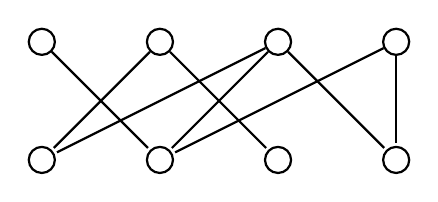
\begin{tikzpicture}[-,>=stealth,shorten >=1pt,auto,node distance=1.5cm, thick,main node/.style={scale=0.9,circle,draw,font=\sffamily\normalsize}]

            \node[circle, draw] (1) []{};
            \node[circle, draw] (2) [right of = 1]{};
            \node[circle, draw] (3) [right of = 2]{};
            \node[circle, draw] (4) [right of = 3]{};
            \node[circle, draw] (5) [below of = 1]{};
            \node[circle, draw] (6) [below of = 2]{};
            \node[circle, draw] (7) [below of = 3]{};
            \node[circle, draw] (8) [below of = 4]{};

            \draw[-] (1) to (6);
            \draw[-] (2) to (5);
            \draw[-] (2) to (7);
            \draw[-] (3) to (5);
            \draw[-] (3) to (6);
            \draw[-] (3) to (8);
            \draw[-] (4) to (6);
            \draw[-] (4) to (8);

            ;
        \end{tikzpicture}
        \caption{An example of a \tit{bipartite graph}. In particular, if we call the uppermost set of nodes $A$ and the lowermost one $B$, then $(A, B)$ is a bipartition of the graph.}
        % \label{}
    \end{figure}

    The graph $K_{a, b}$ is the \tit{complete bipartite} graph bipartitioned through $(A, B)$ such that $\abs A = a$ and $\abs B = b$.

    There are various types of graphs that can be bipartitioned. For example, any \tbf{tree} $T$ can be bipartitioned through a bipartition $(X, V(T) - X)$ by considering the following set of vertices $$X := \{v \in V(T) \mid \dist(r, v) \ \mathrm{even}\}$$ where $r$ is $T$'s root.

    \begin{figure}[H]
        \centering
        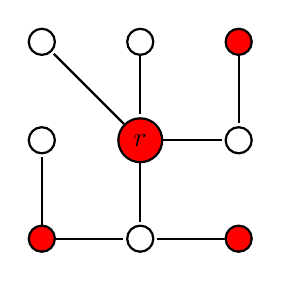
\begin{tikzpicture}[-,>=stealth,shorten >=1pt,auto,node distance=1.25cm, thick,main node/.style={scale=0.9,circle,draw,font=\sffamily\normalsize}]

            \node[circle, draw] (1) []{};
            \node[circle, draw, fill=red] (2) [right of = 1]{};
            \node[circle, draw, fill=red] (3) [below of = 1]{$r$};
            \node[circle, draw] (4) [below of = 2]{};
            \node[circle, draw] (5) [left of = 1]{};
            \node[circle, draw] (6) [below of = 3]{};
            \node[circle, draw, fill=red] (7) [right of = 6]{};
            \node[circle, draw, fill=red] (8) [left of = 6]{};
            \node[circle, draw] (9) [above of = 8]{};

            % \draw[-] (1) to (2);
            \draw[-] (1) to (3);
            \draw[-] (2) to (4);
            % \draw[-] (1) to (5);
            \draw[-] (3) to (4);
            \draw[-] (3) to (5);
            \draw[-] (3) to (6);
            \draw[-] (7) to (6);
            \draw[-] (8) to (6);
            \draw[-] (8) to (9);

            ;
        \end{tikzpicture}
        \caption{The set of red vertices $X$ defines a bipartition $(X, V(T) - X)$ of this tree $T$.}
    \end{figure}

    However, \tit{not every type} of graph can be bipartitioned. For instance, consider the following type.

    \begin{frameddefn}{Clique}
        A \tbf{clique} is a \tit{graph} in which each vertex is adjacent to any other vertex of the graph. A clique that has $n$ vertices --- referred to as $k$-clique --- is denoted as $K_n$.
    \end{frameddefn}

    \begin{figure}[H]
        \centering
        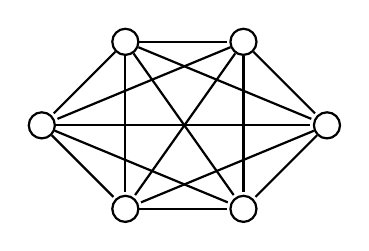
\begin{tikzpicture}[-,>=stealth,shorten >=1pt,auto,node distance=1.5cm, thick,main node/.style={scale=0.9,circle,draw,font=\sffamily\normalsize}]

            \node[circle, draw] (1) []{};
            \node[circle, draw] (2) [right of = 1]{};
            \node[circle, draw] (3) [below left of = 1]{};
            \node[circle, draw] (4) [below right of = 2]{};
            \node[circle, draw] (5) [below right of = 3]{};
            \node[circle, draw] (6) [below left of = 4]{};

            \draw[-] (1) to (2);
            \draw[-] (1) to (3);
            \draw[-] (1) to (4);
            \draw[-] (1) to (5);
            \draw[-] (1) to (6);
            \draw[-] (2) to (3);
            \draw[-] (2) to (4);
            \draw[-] (2) to (5);
            \draw[-] (2) to (6);
            \draw[-] (3) to (4);
            \draw[-] (3) to (5);
            \draw[-] (3) to (6);
            \draw[-] (4) to (5);
            \draw[-] (4) to (6);
            \draw[-] (5) to (6);

            ;
        \end{tikzpicture}
        \caption{The clique $K_6$.}
        % \label{}
    \end{figure}

    It is easy to see that no clique $K_n$ can be bipartitioned, since there is an edge between any pair of vertices of the graph. However, this is not the only type of graph that cannot be bipartitioned.

    \begin{framedlem}{}
        If $G$ is a bipartite graph, and $H$ is a subgraph of $G$, then $H$ must be bipartite.
    \end{framedlem}
    
    \begin{proof}
        Given a bipartite graph $G = (V, E)$, assume that $(X, V - X)$ is a bipartition of $G$, and let $H$ be a subgraph of $G$; then, it is easy to see that $(X \cap V(H), V(H) - X)$ is a bipartition for $H$.
    \end{proof}

    Note that this lemma implies that $G$ is bipartite if and only if every connected component of $G$ is bipartite: in fact, the direct implication follows from this lemma, and the following figure provides an intuition for the converse implication.

        \begin{figure}[H]
        \centering
        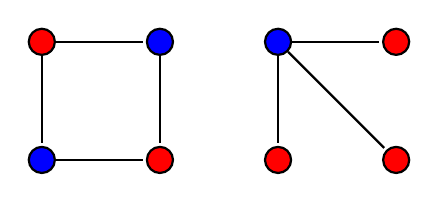
\begin{tikzpicture}[-,>=stealth,shorten >=1pt,auto,node distance=1.5cm, thick,main node/.style={scale=0.9,circle,draw,font=\sffamily\normalsize}]

            \node[circle, draw, fill=red] (1) []{};
            \node[circle, draw, fill=blue] (2) [right of = 1]{};
            \node[circle, draw, fill=blue] (3) [below of = 1]{};
            \node[circle, draw, fill=red] (4) [right of = 3]{};
            \node[circle, draw, fill=blue] (5) [right of = 2]{};
            \node[circle, draw, fill=red] (6) [right of = 5]{};
            \node[circle, draw, fill=red] (7) [below of = 5]{};
            \node[circle, draw, fill=red] (8) [right of = 7]{};

            \draw[-] (1) to (2);
            \draw[-] (1) to (3);
            \draw[-] (2) to (4);
            \draw[-] (3) to (4);

            \draw[-] (5) to (6);
            \draw[-] (5) to (7);
            \draw[-] (5) to (8);

            ;
        \end{tikzpicture}
        \caption{Consider the following disconnected graph $G$ made of these two connected components, $C_1$ and $C_2$ respectively. Say that $C_1$ has a bipartition $(X_1, V(C_1) - X_1)$ where $X_1$ is the red set, and $C_2$ has a bipartition $(X_2, V(C_2) - X_2)$ where $X_2$ is the red set; thus, $(X_1 \cup X_2, V(C_1 \cup C_2) - X_1 - X_2)$ is clearly a bipartition of $G$. This process may be repeated for all the connected components of any disconnected graph.}
        % \label{}
    \end{figure}

    \begin{framedthm}[label={odd-len bip}]{}
        $G$ is bipartite if and only if $G$ has no odd-length cycle.
    \end{framedthm}

    \proofiff{
        We will prove the contrapositive, i.e. if $G$ has an odd-length cycle, then $G$ cannot be bipartitioned. Consider a graph $G$ with an odd-length cycle $C_{2k + 1}$ of vertices $x_1, \ldots, x_{2k + 1}$; by way of contradiction, assume that $G$ is bipartite through a bipartition $(X, V(G) - X)$ for some $X \subseteq V(G)$. Without loss of generality assume that $x_1 \in X$; then, since $X$ defines a bipartition of $G$ it must be that $x_2 \notin X$, and $x_3 \in X$ and so on and so forth. In particular, for any odd value of $i$ we will have that $x_i \in X$, but this implies that both $x_1$ and $x_{2k + 1}$ must be inside $X$, which means that the edge $x_1x_{2k + 1}$ violates the bipartition induced by $X$ $\lightning$.
    }{
        Again, we will prove the contrapositive, i.e. if $G$ is not bipartite it must contain an odd-length cycle. By the previous observation, $G$ is not bipartite if and only if at least one connected component of $G$ is not bipartite, and let this component be $\overline G$. Note that, since $\overline G$ is connected, it must contain a spannning tree $T$ by \cref{spanning tree existence}. Moreover, as previously described, we can always define a bipartition on a tree, namely $(X, V(T) - X)$ where $$\textstyle X := \{v \in V(T) \mid \dist_T(r, v) \ \mathrm{even}\}$$ for some root node $r \in V(T)$.

        Now, since $T$ is a spanning tree of $\overline G$, which is now bipartite by hypothesis, there must be an edge $xy \in V(\overline G)$ such that either $x, y \in X$ or $x, y \in V(T) - X$, i.e. the edge $xy$ must have both endpoints in the same set of $T$'s bipartition. Let $z$ be the LCA between $x$ and $y$ in $T$, and $P_x$ and $P_y$ be the paths of the form $x \to r$ and $y \to r$, respectively. Note that, since $xy$ has both endpoints in the same set, it must be that the lengths of $P_x$ and $P_y$ have the same parity by definition of $X$. Lastly, by statement 2 of \cref{tree alt} we have that $r \ P_x \ z = r \ P_y \ z$, which implies that the lengths of $z \ P_x \ x$ and $z \ P_y \ y$ must have the same parity. This concludes that $$z \ P_x \ x \cup z \ P_y \ y \cup xy$$ is an odd-length cycle of $G$.
    }

    \subsection{Eulerian tours}

    At the start of this chapter, we introduced the \tit{Seven Bridges of Königsberg} problem, which led to the emergence of graph theory as a branch of combinatorics. Over time, as the field developed, this problem was formalized into the following definition.

    \begin{frameddefn}{Eulerian tour}
        An \tbf{Eulerian tour} over a graph $G$ is a closed walk that traverses every edge of $G$ exactly once.
    \end{frameddefn}

    For instance, consider the following graph

    \begin{figure}[H]
        \centering
        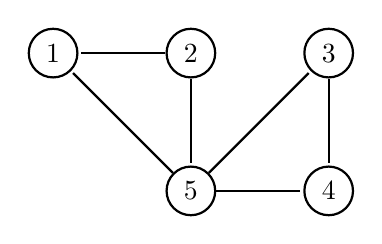
\begin{tikzpicture}[-,>=stealth,shorten >=1pt,auto,node distance=1.75cm, thick,main node/.style={scale=0.9,circle,draw,font=\sffamily\normalsize}]

            \node[circle, draw] (1) []{2};
            \node[circle, draw] (2) [right of = 1]{3};
            \node[circle, draw] (3) [below of = 1]{5};
            \node[circle, draw] (4) [below of = 2]{4};
            \node[circle, draw] (5) [left of = 1]{1};

            \draw[-] (3) to (2);
            \draw[-] (1) to (3);
            \draw[-] (2) to (4);
            \draw[-] (1) to (5);
            \draw[-] (3) to (4);
            \draw[-] (3) to (5);

            ;
        \end{tikzpicture}
        % \caption{A simple graph.}
        % \label{first graph}
    \end{figure}

    After some trial an error, it is easy to find an Eulerian tour over this graph, for instance $$1 \ \{1, 2\} \ 2 \ \{2, 5\} \ 5 \ \{5, 3\} \ 3 \ \{3, 4\} \ 4 \ \{4, 5\} \ 5 \ \{5, 1\} \ 1$$ Note that this is a valid Eulerian tour because there is no edge repetition, and vertex repetition is allowed by definition. On the counter side, the graph --- or, more precisely, the \tit{multigraph} --- that the bridges of Königsberg define, which is the following

    \begin{figure}[H]
        \centering
        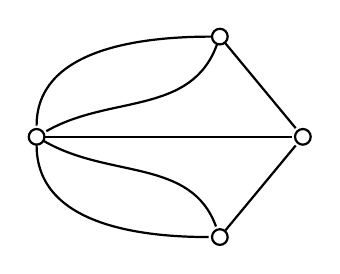
\begin{tikzpicture}[-,>=stealth,shorten >=1pt,auto,node distance=3cm,thick,main node/.style={scale=0.6,circle,draw,font=\sffamily\normalsize}]
            \node[main node] (1) {};
            \node[main node] (2) [below left of=1, xshift = -50] {};
            \node[main node] (3) [below right of=2, xshift = 50] {};
            \node[main node] (4) [right of=2, xshift = 75] {};

            \path[every node/.style={font=\sffamily\small}]
                (1) edge [out=180, in=90] (2)
                (1) edge [out=-110, in=30] (2)
                (2) edge [out=270, in=180] (3)
                (2) edge [out=-30, in=110] (3)
                (2) edge (4)
                (1) edge (4)
                (3) edge (4)
                ;
        \end{tikzpicture}
        % \caption{The graph drawn by Euler which models the \tit{Seven Bridges of Königsberg} problem.}
        % \label{konigsberg}
    \end{figure}

    does not admit any Eulerian tour. But, given a graph, how can we determine with certainty whether it contains an Eulerian tour? The following theorem, proved by Euler himself in his original paper \cite{konigsberg}, answers this question. Note that this theorem holds both for graphs and multigraph.

    \begin{framedthm}{Eulerian tours}
        A graph $G$ admits an Eulerian tour if and only $G$ is connected and every vertex of $G$ has even degree.
    \end{framedthm}
    
    \proofiff{
        Consider the contrapositive of the direct implication, and assume that $G$ contains at least one odd-degree vertex $v$. Recall that an Eulerian tour is a closed walk that does not allow edge repetition, which implies that the \tit{starting} point of the walk is actually not relevant. Therefore, we can assume without loss of generality that any possible Eulerian tour defined on $G$ starts on $v$ itself, but then to be \tit{closed} it must end on $v$ as well. Moreover, each time any Eulerian tour passes through $v$ it must use 2 distinct edges, however $v$ is an odd-degree vertex, therefore at the end of the Eulerian tour there is no way we can come back to $v$ and close the walk.
    }{
        Consider a graph $G$ in which every vertex has even degree, and let $W$ be the \tit{longest} walk of $G$ that does not repeat edges, and let it be labeled as follows $$x_0 \ e_1 \ x_1 \ \ldots \ x_{k - 1} \ e_k \ x_k$$ 

        \claim{
            $x_0 = x_k$, i.e. $W$ is closed.
        }{
            By way of contradiction, assume that $W$ $x_0 \neq x_k$. If this is the case, then $x_k = v$ for some vertex $v$ that is not $x_0$. Note that $W$ is a \tit{walk}, therefore $v$ may be repeated multiple times inside $W$, i.e. $$x_0 \ e_1 \ x_1 \ \ldots \ v \ \ldots \ v \ \ldots \ x_{k - 1} \ e_k \ v$$ If $l$ is the number of times $v$ occurs in $W$ \tit{without counting} $x_k$, then clearly in $W$ there are $2l + 1$ edges incident to $v$, namely $e_k$ and 2 edges each other time $v$ appears in $W$. However, since $2l + 1$ is odd and we assumed that $G$ has no odd-degree vertices, there must be at least one edge $vu \in E(G)$ such that $u \notin V(W)$. This implies that $$x_0 \ e_1 \ x_1 \ \ldots \ x_{k - 1} \ e_k \ v \ vu \ u$$ is a longer walk than $W$, and it does not repeat any edges because $uv \notin E(W)$, contradicting the definition of $W$ $\lightning$.
        }

        This claim proves that $W$ is closed, but we still need to prove that it traverses every edge to claim that it is indeed an Eulerian tour. By way of contradiction, assume that there exists at least one edge $e \notin E(W)$ not used by $W$. Consider an vertex $x_i$ of $W$; by connectivity of $G$, there must be a path $P$ beween $x_i$ and each of the endpoints of $e$. Let $x_i u$ be the first edge of $P$, for some $u \notin E(W)$. This implies that $$u \ ux_i \ x_i \ e_{i + 1} \ x_{ i+ 1} \ \ \ldots \ x_{k - 1} \ e_k \ x_k \ e_1 \ x_1 \ \ldots \ x_{i - 1} \ e_i \ x_i$$ is a longer walk than $W$ that does not repeat any edge, since $ux_i \notin E(W)$, again contradicting the definition of $W$ $\lightning$.
    }

    Note that this theorem proves that it is not possible to describe an Eulerian tour over the bridges and landmasses of Königsberg, because every vertex of the multigraph has odd degree.

    \subsection{Hamiltonian cycles}
    
    Eulerian tours are closed walks that traverse every edge of the graph exactly once. But what if we are interested in traversing each \tit{vertex} exactly once instead?

    \begin{frameddefn}{Hamiltonian paths and cycles}
        A \tbf{Hamiltonian path} over a graph $G$ is a subgraph $P_n$ of $G$. A \tbf{Hamiltonian cycle} over a graph $G$ is a subgraph $C_n$ of $G$.
    \end{frameddefn}

    Hamiltonian paths and cycles are named after \href{https://en.wikipedia.org/wiki/William_Rowan_Hamilton}{W. R. Hamilton}. Note that the notation $P_n$ (or $C_n$) implies that the length of the path (or cycle) is $n$, hence this definition matches our requirements.

    As for the case of Eulerian tours, when some conditions are met, Hamiltonian cycles are guaranteed to exist, as discussed in the following theorem.

    \begin{framedthm}{Hamiltonian cycles}
        A graph $G$ such that $\delta \ge \tfrac{n}{2}$ contains a Hamiltonian cycle.
    \end{framedthm}

    \begin{proof}
        First, we will prove that the condition of the statement implies that $G$ is connected.

        \claim{
            $G$ is connected.
        }{
            By way of contradiction, suppose that $G$ is not connected; therefore $G$ has at least two connected components. Let $H$ be the smallest connected component of $G$; then, clearly $\abs{V(H)} \le \tfrac{n}{2}$. However, note that $\abs{\mathcal N (x)} \ge \delta \ge \tfrac{n}{2}$ and since $\{x\} \cup \mathcal N (x) \subseteq V(H)$, we get that $V(H)$ must have at least $\tfrac{n}{2} + 1$ nodes $\lightning$.
        }

        Let $P$ be the longest path of $G$, and let $x_0, \ldots, x_k$ be its vertices.

        \claim{
            There exists an index $\ell$ such that $x_0 \ x_\ell \ x_{\ell + 1} \ \ldots \ x_{k - 1} \ x_k \ x_{\ell - 1} \ x_{\ell - 2} \ \ldots \ x_1 \ x_0 $ is a cycle.
        }{
            By the same argument used in the proof of \cref{longest path len}, we know that $$\mathcal N(x_0), \mathcal N (x_k) \subseteq \{x_0, \ldots, x_k\}$$ Let $I_0$ and $I_k$ be the following two sets $$I_0 := \{i \mid i \in [1,k], x_i \in \mathcal N (x_0)\} \implies \abs{I_0} = \abs{\mathcal N(x_0)}$$ $$I_k := \{i \mid i \in [1, k], x_{i - 1} \in \mathcal N (x_k)\} \implies \abs{I_k} = \abs{\mathcal N (x_k)}$$ Since $\delta \ge \tfrac{n}{2}$, we have that $\abs{I_0}, \abs{I_k} \ge \tfrac{n}{2}$. However, note that $k \le n - 1$ --- since we started counting at 0 --- hence by the pigeonhole principle there must be at least one index $\ell \in I_0 \cap I_k$, meaning that $x_0 \sim x_\ell$ and $x_k \sim x_{\ell - 1}$, defining a cycle as described in the statement of the claim.
        }

        This means that we found a cycle $C$ in the graph that uses all the vertices of $P$, namely $x_0, \ldots, x_k$. By way of contradiction, assume that $k < n - 1$, i.e. $C$ has less than $n$ nodes, meaning that $C$ is a non-Hamiltonian cycle. In particular, if $k < n - 1$, we have that $\abs{V(G)} - \abs{V(C)} \neq \varnothing$, thus let $y \in V(G) - V(C)$. By the previous claim, we know that $G$ is connected, there must be an edge $xy \in E(G)$ such that $x \in V(C)$. However, this would imply that $P \cup \{xy\}$ is a path of longer path than $P$ $\lightning$.
    \end{proof}

    Note that the statement of this theorem cannot be improved, even by 1; for instance consider the following graph

        \begin{figure}[H]
        \centering
        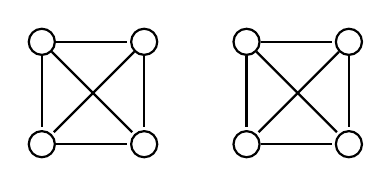
\begin{tikzpicture}[-,>=stealth,shorten >=1pt,auto,node distance=1.3cm, thick,main node/.style={scale=0.9,circle,draw,font=\sffamily\normalsize}]

            \node[circle, draw] (1) []{};
            \node[circle, draw] (2) [right of = 1]{};
            \node[circle, draw] (3) [below of = 1]{};
            \node[circle, draw] (4) [right of = 3]{};

            \node[circle, draw] (5) [right of = 2]{};
            \node[circle, draw] (6) [right of = 5]{};
            \node[circle, draw] (7) [below of = 5]{};
            \node[circle, draw] (8) [right of = 7]{};

            \draw[-] (1) to (2);
            \draw[-] (1) to (3);
            \draw[-] (1) to (4);
            \draw[-] (2) to (3);
            \draw[-] (2) to (4);
            \draw[-] (3) to (4);

            \draw[-] (5) to (6);
            \draw[-] (5) to (7);
            \draw[-] (5) to (8);
            \draw[-] (6) to (7);
            \draw[-] (6) to (8);
            \draw[-] (7) to (8);

            ;
        \end{tikzpicture}
        % \caption{A \tit{matching} of the previous graph.}
        % \label{matching}
    \end{figure}

    composed of two disconnected $K_4$. Here, we have that $$\delta = 4 - 1 = 3 \ge \dfrac{2 \cdot 4}{2} - 1 = 4 - 1 = 3 = \dfrac{n}{2} - 1$$ Therefore, $\delta \ge \tfrac{n}{2} - 1$ is not sufficient to guarantee connectivity.

    \section{Exercises}

    \begin{framedprob}{}
        Let $G = (V, E)$ be a graph of $n$ vertices, where $n \ge 2$. Show that there must be two vertices $x, y \in V$ such that $\deg(x) = \deg(y)$.
    \end{framedprob}

    \solution{
        By definition, the range of the possible degrees for any node of $G$ is $[0, n - 1]$. By way of contradiction, assume that for any two vertices $x, y \in V$ it holds that $\deg(x) \neq \deg(y)$; hence, since the graph has $n$ nodes, it must be that each node is assigned a different degree, and that we use all the possible degrees in $[0, n - 1]$. In particular, this implies that there are two vertices $u, v \in V$ such that $\deg(u) = 0$ and $\deg(v) = n - 1$, but this is a contradiction because if the degree of $v$ is $n - 1$, it must be adjacent to all the other nodes of $V$, including $u$, and $\deg(u) = 0$ $\lightning$.
    }

    \begin{framedprob}{}
        Let $G$ be a graph containing a cycle $C$, and assume that $G$ contains a path of length at least $k$ between two vertiecs of $C$. Show that $G$ contains a cycle of length at least $\sqrt k$. Can this bound be improved?
    \end{framedprob}

    \solution{
        Consider a graph $G$ that contains a cycle $C$, and let $P$ be a path between two vertices $x, y \in V(C)$ such that $\abs{E(P)} \ge k$ for some $k$. Starting from $x$, let $x_1, \ldots, x_t$ be the vertices through which $P$ \curlyquotes{leaves} $C$, and $y_1, \ldots, y_t$ be the vertices through which $P$ \curlyquotes{joins back} $C$. We observe that if $2t \ge \sqrt k$, it means that there are at least $\sqrt k$ vertices in $C$, thus the theorem trivially holds by simply considering $C$ itself, so we may assume that $2t < \sqrt k$.

        Let $P_i := x_i \ P \ y_i$ and $\overline{P_i} := y_i \ P \ x_{i + 1}$, and let $C_i$ be the shortest subpath of $C$ of the form $x_i \ C \ y_i$ --- there are two subpaths of this form. We observe that there are $t$ subpaths of the form $P_i$, and at most $t + 1$ subpaths of the form $\overline{P_i}$, meaning that $P$ can be partitioned in at most $2t + 1$ subpaths of the forms described. Now, let $P^*$ be the subpath of $P$ that maximizes its length --- $P^*$ may be of the form $P_i$ or $\overline P_i$. Hence, we get that $$k \le \abs{E(P)} \le (2t + 1) \abs{E(P^*)} < (\sqrt k + 1) \abs{E(P^*)}$$ and in particular $$\abs{E(P^*)} (\sqrt k + 1) > k \iff \abs{E(P^*)} > \dfrac{k}{\sqrt k + 1} \iff \abs{E(P^*)} \ge \dfrac{k}{\sqrt k + 1} + 1 \ge \sqrt k$$ where the last inequality can be proved as follows $$\dfrac{k}{\sqrt k + 1} + 1 \ge \sqrt k \iff \dfrac{k + \sqrt k + 1}{\sqrt k + 1} \ge \sqrt k \iff k + \sqrt k + 1 \ge \sqrt k (\sqrt k + 1) = k + \sqrt k$$

        Now, if the subpath $P^*$ lies inside $C$, since $\abs{E(P^*)} \ge \sqrt k$ the theorem holds by considering the cycle $C$ itself, so we may assume that there exists $i^* \in [t]$ such that $P_{i^*} = P^*$.

        Lastly, since $P_i$ and $C_i$ do not intersect for each $i \in [t]$, we have that $$\abs{E(P_i \cup C_i)} = \abs{E(P_i)} + \abs{E(C_i)} \ge \abs{E(P_i)} + 1$$ and in particular $$\abs{E(P_{i^*} \cup C_{i^*})} \ge \sqrt k + 1 \ge \sqrt k$$ which means that

        \begin{itemize}
            \item $P_{i^*} \cup C_{i^*}$ is the cycle that proves the statement
            \item we can improve the bound of the statement to be at least $\sqrt k + 1$
        \end{itemize}
    }

    \begin{framedprob}{Tree-order}
        Consider a tree $T$, and let $r \in V(T)$ be its root. We define the \tbf{tree-order} $\le_r$ associated with $r$ as follows: $$\forall x, y \in V(T) \quad x \le_r y \iff x \in V(r \ T \ y)$$ Prove that

        \begin{enumerate}
            \item $r$ is the least element in this partial order.
            \item Every leaf different from $r$ is a maximal element.
            \item the endpoints of any edge of $T$ are comparable.
            \item For any $y \in V(T)$, every set of the form $\{x \in V(T) \mid x \le_r y\}$ is a \tit{chain}, i.e. a set of pairwise comparable elements.
        \end{enumerate}
    \end{framedprob}

    \solution{
        We can prove the statements by using the properties of trees.

        \begin{enumerate}
            \item By way of contradiction, suppose that there is an element $m$ such that $m \le_r r$ and $m \neq r$; by definition, this happens if and only if $m \in V(r \ T \ r) = \{r\}$, meaning that $m = r$ $\lightning$.
            \item By way of contradiction, let $l \neq r$ be a leaf of $T$ that is not maximal, i.e. there is a node $v \in V(T)$ such that $l \le_r v$ and $l \neq v$. By definition, this can happen if and only if $l \in V(r \ T \ v)$, but if $l \neq v$ and $l$ is in a path $r \to v$, then $\deg(l) \ge 2$ contradicting the fact that $l$ was a leaf of $T$ $\lightning$.
            \item Fix an edge $e \in E(T)$; we can label the endpoints of $e$ with $x$ and $y$ such $\dist(r, y) = \dist(r, x) + 1$ --- i.e. $x$ \curlyquotes{comes before} $y$ in the path $r \to y$ --- and this suffices to show that $x \in V(r \ T \ y) \iff x \le_r y$.
            \item Let $y \in V(T)$, and fix a set $S_y := \{x \in V(T) \mid x \le_r y\}$. We observe that $x \le_r y \iff x \in V(r \ T \ y)$, which implies that $x \in S_y \iff x \in V(r \ T \ y)$ meaning that $S_y = V(r \ T \ y)$. Then, fix a pair of distinct elements $a, b \in S_y$, and without loss of generality suppose that $b$ is the element that maximizes the distance from $r$. We observe that $S_y = V(r \ T \ y)$ implies that for any $x \in S_y$ the path $r \ T \ y$ contains $r \ T \ x$, and in particular it contains both $r \ T \ a$ and $r \ T \ b$. Moreover, since $b$ is further from $r$ than $a$, the path $r \ T \ a$ is contained in $r \ T \ b$, which means that $a \in V(r \ T \ b) \iff a \le_r b$.
        \end{enumerate}
    }

    \begin{framedprob}{}
        Show that every connected graph $G$ contains a path of length at least $\min\{2 \delta, n - 1\}$.
    \end{framedprob}

    \solution{
        Let $P$ be the longest path of vertices $x_1 \ \ldots \ x_k$. If $\abs{V(P)} = n$ then $\abs{E(P)} = n - 1 \ge \min\{2 \delta, n - 1\}$, so we may assume that $\abs{V(P)} \le n - 1$.

        \claim{
            If $x_i \in \mathcal N(x_1)$, then $x_{i - 1} \notin \mathcal N(x_k)$.
        }{
            By way of contradiction, suppose that there is an index $j$ such that $x_1 \sim x_j$ and $x_{j - 1} \sim x_k$; then $$x_1 \ \ldots \ x_{j - 2} \ x_{j - 1} \ x_k \ x_{k - 1} \ \ldots \ x_{j + 1} \ x_j \ x_1$$ is a cycle --- call this cycle $C$. Since we are assuming that $\abs{V(P)} \le n - 1$, there must be at least another vertex $z \in V(G) - V(P)$. By connectivity of $G$, we know that there is a path $Q$ from $z$ to some vertex $v_i \in V(C)$; hence, we have that $$Q \cup x_i \ x_{i + 1} \ \ldots \ x_k \ x_1 \ \ldots \ x_{i - 1}$$ is a path containing more vertices than the vertices of $P$, contradicting the maximality of $\abs{E(P)}$ $\lightning$.
        }
        
        We observe that $\mathcal N(x_1) , \mathcal N(x_k) \subseteq V(P) = \{x_1, \ldots, x_k\}$, otherwise we would contradict the maximality of $P$. Let $\mathcal N(x_1) = \{x_{i_1}, \ldots, x_{i_\ell}\}$; by the previous claim, we get that $$\mathcal N(x_k) \subseteq \{x_2, \ldots, x_k\} - \{x_{i_1 - 1} , \ldots, x_{i_\ell - 1}\}$$ therefore $$\delta \le \abs{\mathcal N(x_k)} \le k - 1 - \abs{\mathcal N(x_1)} \le k - 1 - \delta$$ meaning that $k \ge 2 \delta + 1 \implies \abs{E(P)} \ge 2\delta \ge \min\{2 \delta, n -1\}$.
    }

    \begin{framedprob}{}
        Show that every tree $T$ has at least $\Delta(T)$ leaves.
    \end{framedprob}

    \solution{
        Consider a vertex $v$ of maximum degree, i.e. $\deg(v) = \Delta(T)$.

        \claim{
            There are $\Delta(T)$ connected components in $T[V(T) - \{v\}]$.
        }{
            By way of contradiction suppose that there are less than $\Delta(T)$ components in this subgraph. However, by pigeonhole principle, since there are $\Delta(T)$ edges incident to $v$, and less than $\Delta(T)$ components, there must be two neighbors of $v$ --- say $x$ and $y$ --- lying in the same component of $T[V(T) - \{v\}]$. However, since the component is connected by definition, there is a path between $x$ and $y$, say $P$, which implies that $v \ \{v, x\} \ P \ y \ \{y, v\} \ v$ is a cycle, contradicting the fact that $T$ was a tree.

            Finally, if there are more than $\Delta(T)$ components when removing $v$ from $T$, it meant that at least one component was already present in $T$, meaning that $T$ had at least 2 different components, contradicting the fact that $T$ was a tree.
        }

        Moreover, since $T$ is a tree, each of the $\Delta(T)$ components in $T[V(T) - \{v\}]$ must be both connected and acyclic, implying that all of these components are trees themselves. Lastly, for each subtree we have two cases:

        \begin{itemize}
            \item if the subtree has 1 vertex, the subtree was a leaf of $T$
            \item else, if the subtree has at least 2 vertices, by \cref{leaf existence} the subtree contains at least one leaf
        \end{itemize}

        and in both cases each subtree contains at least one leaf, meaning that $T$ contains at least $\Delta(T)$ leaves.
    }
    
    \begin{framedprob}{}
        Show that any non-trivial tree without a vertex of degree 2 has more leaves than other vertices. Can you find a very short proof that does not use induction?
    \end{framedprob}

    \solution{
        Let $T$ be a non-trivial tree that does not contain vertices of degree 2, and let $L = \{v \in V(T) \mid \deg(v) = 1\}$ the set of its leaves. By the Handshaking lemma, we know that
        \begin{equation*}
            \begin{split}
                2 \abs{E(T)} &= \sum_{v \in V(T)}{\deg(v)} \\
                             &= \sum_{v \in V(T) - L}{\deg(v)} + \sum_{v \in L}{\deg(v)} \\
                             &\ge \abs L + 3 \abs{V(T) - L}
            \end{split}
        \end{equation*}
        Moreover, since $T$ is a tree, we have that $$2 \abs{E(T)} = 2(n - 1) = 2(\abs L + \abs{V(T) - L} - 1) = 2 \abs L + 2 \abs{V(T) - L} - 2$$ Therefore, we have that $$2 \abs L + 2 \abs{V(T) - L} - 2 \ge \abs L + 3 \abs{V(T) - L}$$ implying that $\abs L \ge \abs{V(T) - L} + 2 \iff \abs L > \abs{V(T) - L} + 1$.
    }

    % \begin{framedprob}{}
    %     Let $\mathcal T := \{T_1, \ldots, T_k\}$ be a set of subtrees of a tree $T$. ASsume that the trees in $\mathcal T$ have pairwise non-empty intersection. Show that their overall intersection $\bigcap_{i = 1}^k{V(T_i)}$ is non-empty.
    % \end{framedprob}
    %
    % \solution{
    %     If $k = 1$, i.e. $\mathcal T = \{T_1\}$, the implication is vacuously true. Moreover, if $k = 2$ we have that $T_1 \cap T_2 \neq \varnothing$ meaning that the theorem trivially holds. However, we observe that the intersection between $T_1$ and $T_2$ cannot contain more than one single vertex. In fact, suppose that $T_1 \cap T_2 = \{x, y\}$ for some vertice $x \neq y$: then, by connectivity of $T_1$ there is a path $P_1$ of the form $x \to y$ in $T_1$, and by connectivity of $T_2$ there is a path $P_2$ of the form $x \to y$ in $T_2$, meaning that $P_1 \cup P_2$ is a cycle in $T$, which is impossible since $T$ is a tree. This observation implies that if $T_i \cap T_j \neq \varnothing$, then $\abs{T_i \cap T_j} = 1$.
    %
    %     By way of contradiction, suppose that the pairwise intersection of the trees in $\mathcal T$ is non-empty, but thei overall intersection is empty. If this is the case, it means that there is no vertex which belongs to all the subtrees in $\mathcal T$, 
    % }

    \chapter{Matchings}

    \begin{frameddefn}{Matching}
        Given a graph $G = (V, E)$, a \tbf{matching} of $G$ is a set of edges $M \subseteq E$ such that $$\forall e, e' \in M \quad e \cap e' = \varnothing$$
    \end{frameddefn}

    \begin{figure}[H]
        \centering
        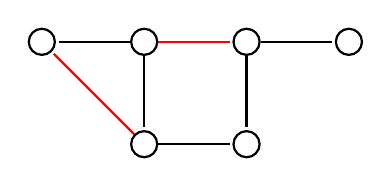
\begin{tikzpicture}[-,>=stealth,shorten >=1pt,auto,node distance=1.3cm, thick,main node/.style={scale=0.9,circle,draw,font=\sffamily\normalsize}]

            \node[circle, draw] (1) []{};
            \node[circle, draw] (2) [right of = 1]{};
            \node[circle, draw] (3) [below of = 1]{};
            \node[circle, draw] (4) [below of = 2]{};
            \node[circle, draw] (5) [left of = 1]{};
            \node[circle, draw] (6) [right of = 2]{};

            \draw[-] (1) [red] to (2);
            \draw[-] (1) to (3);
            \draw[-] (2) to (4);
            \draw[-] (1) to (5);
            \draw[-] (3) to (4);
            \draw[-] (3) [red] to (5);
            \draw[-] (2) to (6);

            ;
        \end{tikzpicture}
        \caption{A \tit{matching} of the previous graph.}
        \label{matching}
    \end{figure}

    As shown in figure, a matching is nothing more than a set of edges that must not share endpoints with each other — for this reason, in literature it is often referred to as \tbf{independent edge set}. 

    Given a matching $M$ in a graph $G$, we say that a vertex $v \in V(G)$ is \tbf{free} w.r.t. $M$ if there are no edges $e \in M$ such that $e \cap v \neq \varnothing$. An edge $xy \in E(G)$ is said to be \tit{disjoint} from $M$ if both $x$ and $y$ are free w.r.t. $M$.

    In graph theory we are often interested in the matching that has the largest possible cardinality of a graph. For this purpose, we often distinguish the two following concepts, namely \tit{maximal} and \tit{maximum} matching.

    \begin{frameddefn}{Maximal matching}
        A \tbf{maximal matching} is a matching that cannot be extended any further.
    \end{frameddefn}
    
    For instance, the matching shown in \cref{matching} is actually a \tbf{maximal matching}, because no other edge in $E$ can be added to che current set of edges $M$ of the matching without breaking the matching condition.

    \begin{frameddefn}{Maximum matching}
        A \tbf{maximum matching} is a matching that has the largest cardinality.
    \end{frameddefn}

    Clearly, the previous example does not repreent a \tbf{maximum matching}, because the following set of edges

     \begin{figure}[H]
        \centering
        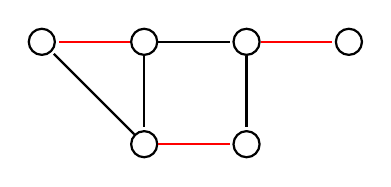
\begin{tikzpicture}[-,>=stealth,shorten >=1pt,auto,node distance=1.3cm, thick,main node/.style={scale=0.9,circle,draw,font=\sffamily\normalsize}]

            \node[circle, draw] (1) []{};
            \node[circle, draw] (2) [right of = 1]{};
            \node[circle, draw] (3) [below of = 1]{};
            \node[circle, draw] (4) [below of = 2]{};
            \node[circle, draw] (5) [left of = 1]{};
            \node[circle, draw] (6) [right of = 2]{};

            \draw[-] (1) to (2);
            \draw[-] (1) to (3);
            \draw[-] (2) to (4);
            \draw[-] (1) [red] to (5);
            \draw[-] (3) [red] to (4);
            \draw[-] (3) to (5);
            \draw[-] (2) [red] to (6);

            ;
        \end{tikzpicture}
    \end{figure}

    is still a valid matching for the graph, but has a larger cardinality than the previous set.

    Given a matching $M$ in a graph $G$, what conditions must be met to increase its cardinality? Trivially, if there exists an edge $e$ disjoint from $M$, clearly $M \cup \{e\}$ is a larger matching than $M$ --- implying that $M$ was not \tit{maximal} in $G$. However, this is not the only situation in which the cardinality of $M$ can be extended. In fact, consider the following definitions.

    \section{Augmenting paths}

    \begin{frameddefn}{Alternating path}
        Given a graph $G$, and a matching $M$ on $G$, an \tbf{$M$-alternating path} is a path of $G$ that starts at a free node w.r.t. $M$, and is composed of edges that alternate between $M$ and $E(G) - M$.
    \end{frameddefn}

    \begin{figure}[H]
        \centering
        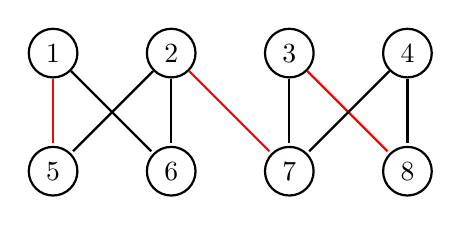
\begin{tikzpicture}[-,>=stealth,shorten >=1pt,auto,node distance=1.5cm, thick,main node/.style={scale=0.9,circle,draw,font=\sffamily\normalsize}]

            \node[circle, draw] (1) []{1};
            \node[circle, draw] (2) [right of = 1]{2};
            \node[circle, draw] (3) [right of = 2]{3};
            \node[circle, draw] (4) [right of = 3]{4};
            \node[circle, draw] (5) [below of = 1]{5};
            \node[circle, draw] (6) [below of = 2]{6};
            \node[circle, draw] (7) [below of = 3]{7};
            \node[circle, draw] (8) [below of = 4]{8};

            \draw[-] (1) [red] to (5);
            \draw[-] (1) to (6);
            \draw[-] (2) to (6);
            \draw[-] (2) to (5);
            \draw[-] (2) [red] to (7);
            \draw[-] (3) to (7);
            \draw[-] (3) [red] to (8);
            \draw[-] (4) to (7);
            \draw[-] (4) to (8);

            ;
        \end{tikzpicture}
        \caption{For instance, if $M$ is the set of \tit{red} edges --- which forms a matching of the graph --- then $6 \ \{6, 2\} \ 2 \ \{2, 7\} \ 7 \ \{7, 3\} \ 3 \ \{3, 8\} \ 8$ is an $M$-alternating path.}
        % \label{}
    \end{figure}
    
    \begin{frameddefn}{Augmenting path}
        Given a graph $G$, and a matching $M$ on $G$, an \tbf{$M$-augmenting path} is an $M$-alternating path that ends at a free vertex w.r.t. $M$.
    \end{frameddefn}

    For example, if we consider the path $$6 \ \{6, 2\} \ 2 \ \{2, 7\} \ 7 \ \{7, 3\} \ 3 \ \{3, 8\} \ 8 \ \{8, 4 \} \ 4$$ this is actually an $M$-augmenting path of the previous graph. Augmenting paths are very useful because they can be used to \tit{expand} the cardinality of an initial matching. In fact, in the previous graph we can actually define a \tit{larger} matching by \tbf{swapping} the edges of this augmenting path, as shown below

    \begin{figure}[H]
        \centering
        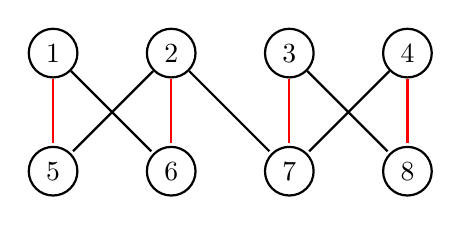
\begin{tikzpicture}[-,>=stealth,shorten >=1pt,auto,node distance=1.5cm, thick,main node/.style={scale=0.9,circle,draw,font=\sffamily\normalsize}]

            \node[circle, draw] (1) []{1};
            \node[circle, draw] (2) [right of = 1]{2};
            \node[circle, draw] (3) [right of = 2]{3};
            \node[circle, draw] (4) [right of = 3]{4};
            \node[circle, draw] (5) [below of = 1]{5};
            \node[circle, draw] (6) [below of = 2]{6};
            \node[circle, draw] (7) [below of = 3]{7};
            \node[circle, draw] (8) [below of = 4]{8};

            \draw[-] (1) [red] to (5);
            \draw[-] (1) to (6);
            \draw[-] (2) [red] to (6);
            \draw[-] (2) to (5);
            \draw[-] (2) to (7);
            \draw[-] (3) [red] to (7);
            \draw[-] (3) to (8);
            \draw[-] (4) to (7);
            \draw[-] (4) [red] to (8);

            ;
        \end{tikzpicture}
        % \caption{For instance, if $M$ is the set of \tit{red} edges --- which forms a matching of the graph --- then $6 \ \{6, 2\} \ 2 \ \{2, 7\} \ 7 \ \{7, 3\} \ 3 \ \{3, 8\} \ 8$ is an $M$-alternating path.}
        % \label{}
    \end{figure}

    \subsection{Berge's theorem}

    This suggests that the presence of augmenting paths in a graph is a \tit{sufficient} condition for a matching \tit{not} to be maximum, but we can actually prove that it is also \tit{necessary}, as stated in the following theorem, proved by \textcite{berge} in 1957.

    \begin{framedthm}[label={aug paths}]{Berge's theorem}
        Given a graph $G$, $M$ is a maximum matching of $G$ if and only if in $G$ there are no $M$-augmenting paths.
    \end{framedthm}

    \proofiff{
        By contrapositive, consider a graph $G$ and a matching $M$ such that there is an $M$-augmenting path $P$ in $G$. Moreover, by way of contradiction assume that $M$ is maximum; however $M \Delta E(P)$ is a larger matching than $M$ --- here, $\Delta$ is the \href{https://en.wikipedia.org/wiki/Symmetric_difference}{symmetric difference}, therefore the operation $M \Delta E(P)$ has the same effect of \tit{swapping} the edges of $P$ between the ones in $M$ and in $E(P) - M$.
    }{
        By contrapositive, consider a graph $G$ and a matching $M$ of $G$ that is not maximum, i.e. there exists a matching $M^*$ of $G$ such that $\abs M < \abs{M^*}$. Consider the subgraph of $G$ that has the vertices of $V(G)$ and the edges described by $M \Delta M^*$; the symmetric difference of these two sets will yield the set of edges that are either in $M$ or in $M^*$, but not in $M \cap M^*$, therefore this subgraph is \tit{not} a multigraph. Moreover, since $M$ and $M^*$ are both matchings, we have that

        \begin{enumerate}[label={(\arabic*)}]
            \item the degrees of the vertices of this subgraph can be either 0, 1 or 2
            \item in each component of the subgraph the edges \tit{must} alternate between $M$ and $M^*$
        \end{enumerate}

        By the observation (1), we have that each component of the subgraph can be either

        \begin{itemize}
            \item a isolated vertex
            \item a cycle
            \item a path
        \end{itemize}

        and by observation (2), we have that all the cycle components must have \tit{even} length, which implies that they have the same number of edges of $M$ and $M^*$. On the other hand, path components may have either even or odd length; in particular, even-length paths must have the same number of edges of $M$ and $M^*$ --- as for cycle components --- while odd-length paths have a different number of edges of $M$ and $M^*$. However, since $\abs M < \abs{M^*}$, there must be at least one path component of this subgraph such that its edges of $M$ are less than the edges of $M^*$, and this is clearly an $M$-augmenting path.
    }

    Given a graph $G$, and a matching $M$ of $G$, what is the maximum possible value for $\abs M$? To answer this question, we need to introduce the following combinatorial structure.

    \subsection{Kőnig's theorem}

    \begin{frameddefn}{Vertex cover}
        Given a graph $G$, a \tbf{vertex cover} for $G$ is a set of vertices $C \subseteq V(G)$ such that every edge in $G$ is incident to at least one vertex in $C$. Using symbols $$\forall (u, v) \in E(G) \quad u \in C \lor v \in C$$
    \end{frameddefn}

    \begin{figure}[H]
        \centering
        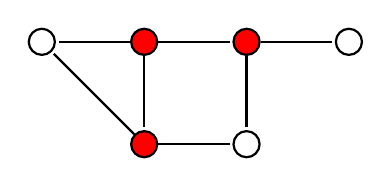
\begin{tikzpicture}[-,>=stealth,shorten >=1pt,auto,node distance=1.3cm, thick,main node/.style={scale=0.9,circle,draw,font=\sffamily\normalsize}]

            \node[circle, draw, fill=red] (1) []{};
            \node[circle, draw, fill=red] (2) [right of = 1]{};
            \node[circle, draw, fill=red] (3) [below of = 1]{};
            \node[circle, draw] (4) [below of = 2]{};
            \node[circle, draw] (5) [left of = 1]{};
            \node[circle, draw] (6) [right of = 2]{};

            \draw[-] (1) to (2);
            \draw[-] (1) to (3);
            \draw[-] (2) to (4);
            \draw[-] (1) to (5);
            \draw[-] (3) to (4);
            \draw[-] (3) to (5);
            \draw[-] (2) to (6);

            ;
        \end{tikzpicture}
        \caption{An example of a vertex cover.}
    \end{figure}
    
    As shown in figure, a vertex cover is simply a set of vertices that must \tit{cover} all the edges of the graph. For vertex covers, we are interested in the \tit{minimum} possible cardinality --- the concepts of \tit{minimal} and \tit{minimum} are defined analogously.

    As introduced before, through vertex covers we can bound the size of any matching of a graph.

    \begin{framedthm}{Matchings bound vertex covers}
        Given a graph $G$, a matching $M$, and a vertex cover $S$ of $G$, it holds that $\abs M \le \abs S$.
    \end{framedthm}

    \begin{proof}
        By definition, any vertex cover $S$ of $G = (V, E)$ is also a vertex cover for $G^B = (V, B)$, for any set of edges $B \subseteq E$, and in particular this is true for $G^M = (V, M)$.

        Now consider $G^M$, and a vertex cover $C$ on it: by construction we have that $\Delta \le 1$, therefore any vertex in $C$ will cover at most 1 edge of $M$. This implies that if $\abs C = k$, then $C$ will cover at most $k$ edges of $G^M$.

        Lastly, since $G^M$ has $\abs M$ edges by definition, any vertex cover defined on $G^M$ has to contain at least $\abs M$ vertices. This implies that no vertex cover $S$ of $G$ smaller than $\abs M$ can exist, because $S$ will have to cover at least the edges in $M$.
    \end{proof}

    \begin{framedcor}{}
        Given a graph $G$, a maximum matching $M^*$ and a minimum vertex cover $S^*$, it holds that $\abs {M^*} \le \abs {S^*}$.
    \end{framedcor}

    Moreover, if the graph is bipartite this theorem is actually \tit{stronger}, as proved by \textcite{konig} in 1931.

    \begin{framedthm}[label={konig}]{Kőnig's theorem}
        Given a bipartite graph $G$, a maximum matching $M^*$ and a minimum vertex cover $S^*$, it holds that $\abs {M^*} = \abs {S^*}$.
    \end{framedthm}

    \begin{proof}
        Consider a graph $G$, a maximum matching $M^*$ and a minimum vertex cover $S^*$ of $G$; by the previous corollary, it follows that to prove the statement it suffices to show that there exists a vertex cover $S$ such that $\abs S = \abs{M^*}$, because $$\abs{M^*} \le \abs{S^*} \le \abs S = \abs{M^*} \implies \abs{M^*} = \abs{S^*}$$ Hence, we are going to construct the following vertex cover. Let $G$ be bipartitioned through $(A, B)$; then, for each edge $ab \in M^*$ such that $a \in A$ and $b \in B$, we place $b \in S$ if and only if there exists an $M^*$-alternating path that starts in $A$ and ends at $b$, otherwise we place $a \in S$.

        \begin{figure}[H]
            \centering
            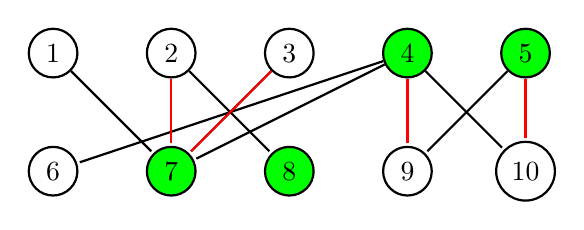
\begin{tikzpicture}[-,>=stealth,shorten >=1pt,auto,node distance=1.5cm, thick,main node/.style={scale=0.9,circle,draw,font=\sffamily\normalsize}]

                \node[circle, draw] (1) []{1};
                \node[circle, draw] (2) [right of = 1]{2};
                \node[circle, draw] (3) [right of = 2]{3};
                \node[circle, draw, fill=green] (4) [right of = 3]{4};
                \node[circle, draw, fill=green] (5) [right of = 4]{5};
                \node[circle, draw] (6) [below of = 1]{6};
                \node[circle, draw, fill=green] (7) [below of = 2]{7};
                \node[circle, draw, fill=green] (8) [below of = 3]{8};
                \node[circle, draw] (9) [below of = 4]{9};
                \node[circle, draw] (10) [below of = 5]{10};

                \draw[-] (1) to (7);
                \draw[-] (2) to (8);
                \draw[-] (3) to (7);
                \draw[-] (4) to (6);
                \draw[-] (4) to (7);
                \draw[-] (4) to (10);
                \draw[-] (5) to (9);

                \draw[-] (2) [red] to (7);
                \draw[-] (3) [red] to (7);
                \draw[-] (4) [red] to (9);
                \draw[-] (5) [red] to (10);

                ;
            \end{tikzpicture}
            \caption{For instance, given this graph bipartitioned into $(A, B)$ --- where $A$ is the uppermost row of vertices --- and the \tit{red} matching, we would construct the \tit{green} vertex cover.}
            % \label{}
        \end{figure}

        Note that, by definition, it holds that $\abs S = \abs{M^*}$.

        \claim{
            $S$ is a vertex cover for $G$.
        }{
            Consider an edge $ab \in E(G)$ such that $a \in A$ and $b \in B$; note that, by definition of $S$ all the edges in $M^*$ are already covered, hence we may assume that $ab \notin M^*$. We have two cases.

            \begin{itemize}
                \item $a$ is free, i.e. $\nexists ab' \in M^*$ for $b' \in B$. Note that $b$ cannot be free, otherwise $M^* \cup \{ab\}$ would still be a matching of $G$ but greater than $M^*$. Hence, there must be an edge $a'b \in M^*$ for some $a' \in A$. Therefore, since $a$ is free, the edge $ab$ is a trivial $M^*$-alternating path ending at $b \in B$, meaning that $b \in S$ by definition, implying that $ab$ is covered by $S$.

                \item $a$ is matched, i.e. $\exists ab' \in M^*$ for $b' \in B$. Therefore, by definition of $S$, either $a$ or $b'$ lies in $S$. In particular, if $a \in S$, then $ab$ is trivially covered by $S$, hence suppose that $b' \in S$.

                    Observe that, by definition of $S$ this implies that there must be an $M^*$-alternating path $P$ that starts in $A$ and ends at $b'$.

                    \begin{itemize}
                        \item If $ab, ab' \notin E(P)$, then $P \cup \{b'a\} \cup ab$ is an $M^*$-augmenting path, which would contradict the fact that $M^*$ is maximum by \cref{aug paths} $\lightning$
                        \item If $ab \notin E(P)$ but $ab' \in E(P)$, then $P$ could not have been an $M^*$-alternating path starting at a vertex in $A$ $\lightning$.
                        \item If $ab \in E(P)$ but $ab' \notin E(P)$, then $P$ must have had the following form $$\ldots \ b'' \ \{b'', a\} \ a \ \{a, b\} \ b \ \{b, a'\} \ a' \ \{a', b'\} \ b'$$ where $a' \in A$, $b'' \in B$. However, since $ab' \in M^*$ and $ab \notin M^*$, and the edges of $P$ must alternate w.r.t. $M^*$, $ab''$ must lie inside $M^*$, contradicting $ab' \in M^*$ by definition of matching $\lightning$.
                    \end{itemize}

                    This implies that $ab', ab \in E(P)$, meaning that $P$ encounters $b$ \curlyquotes{before} $b'$. However, this implies that $P - \{ab'\}$ is an $M^*$-alternating path that starts in $A$ and ends at $b$, thus $b \in S$ by definition, concluding that $ab$ is still covered by $S$.
            \end{itemize}
        }

        Hence, we have constructed a vertex cover $S$ such that $\abs S = \abs{M^*}$, meaning that the statement holds because of the previous observation.
    \end{proof}

    \subsection{Finding maximum matchings}

    Consider a matching $M$ of a graph $G$, and an $M$-augmenting path $P$; the idea of \tit{swapping} the edges of $P$ between $M$ and $E(G) - M$ is very useful when $G$ is \tbf{bipartite}. In fact, we can actually describe a procedure which is able to return a \tit{maximum matching} of a bipartite graph, by swapping the edges of the augmenting paths present in $G$. However, for this algorithm to work, we first need a procedure capable of finding augmenting paths in bipartite graphs, which is defined down below:

    \begin{enumerate}
        \item Assume that the considered graph $G$ is bipartite through $(A, B)$, and consider a matching $M$ of $G$
        \item Starting from a node $a \in A$ free w.r.t. $M$, compute a \tit{modified} BFS such that the edges of its tree alternate between $E(G) - M$ and $M$
        \item If the tree of the BFS contains a free leaf $b \in B$, then the path $v \to b$ is $M$-augmenting
    \end{enumerate}

    For instance, given the following bipartite graph $G$, and a matching $M$ of $G$ --- outlined in \tit{red}

    \begin{figure}[H]
        \centering
        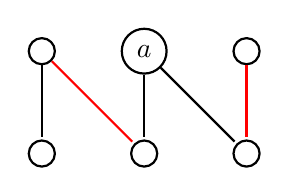
\begin{tikzpicture}[-,>=stealth,shorten >=1pt,auto,node distance=1.3cm, thick,main node/.style={scale=0.9,circle,draw,font=\sffamily\normalsize}]

            \node[circle, draw] (1) []{};
            \node[circle, draw] (2) [right of = 1]{$a$};
            \node[circle, draw] (3) [right of = 2]{};
            \node[circle, draw] (4) [below of = 1]{};
            \node[circle, draw] (5) [right of = 4]{};
            \node[circle, draw] (6) [right of = 5]{};

            \draw[-] (1) to (4);
            \draw[-] (1) [red] to (5);
            \draw[-] (2) to (5);
            \draw[-] (2) to (6);
            \draw[-] (3) [red] to (6);

            ;
        \end{tikzpicture}
        % \caption{An example of a perfect matching.}
    \end{figure}

    the \tit{modified} BFS rooted in $a$ would produce the following tree 

    \begin{figure}[H]
        \centering
        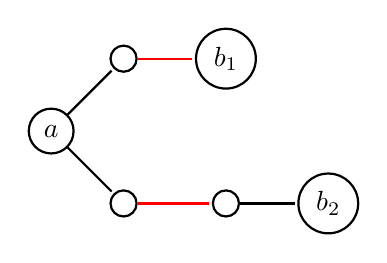
\begin{tikzpicture}[-,>=stealth,shorten >=1pt,auto,node distance=1.3cm, thick,main node/.style={scale=0.9,circle,draw,font=\sffamily\normalsize}]

            \node[circle, draw] (1) []{$a$};
            \node[circle, draw] (2) [above right of = 1]{};
            \node[circle, draw] (3) [right of = 2]{$b_1$};
            \node[circle, draw] (4) [below right of = 1]{};
            \node[circle, draw] (5) [right of = 4]{};
            \node[circle, draw] (6) [right of = 5]{$b_2$};

            \draw[-] (1) to (2);
            \draw[-] (2) [red] to (3);
            \draw[-] (1) to (4);
            \draw[-] (4) [red] to (5);
            \draw[-] (5) to (6);

            ;
        \end{tikzpicture}
        % \caption{An example of a perfect matching.}
    \end{figure}

    and we observe that the path $a \to b_1$ is $M$-alternating, while the path $a \to b_2$ is $M$-augmenting. The next proposition guarantees that if there are $M$-augmenting paths that start in $a$, our \tit{modified} BFS will find at least one of them.

    \begin{framedprop}{}
        Given a bipartite graph $G$, bipartitioned into $(A, B)$, and a matching $M$ of $G$, if there exists an $M$-augmenting path in $G$ that starts in a vertex $a \in A$ free w.r.t. $M$, then there exists an $M$-augmenting path in the tree $T$ of the \tit{modified} BFS.
    \end{framedprop}

    \begin{proof}
        Let $P$ be an $M$-augmenting path that starts in $a$ and minimizes the edges in $E(P) - E(T)$ and, by way of contradiction, assume that $E(P) - E(T) \neq \varnothing$, i.e. $P$ is not completely contained in $T$. Therefore, let $xy$ be the first edge in $E(P) - E(T)$ encountered while traversing $P$, starting at $a$, and without loss of generality assume that $x \in V(P)$.

        \claim{
            $x \in A$.
        }{
            By way of contradiction, assume that $x \in B$.

            \begin{itemize}
                \item Assume that $x$ is not a leaf of $T$. Since the BFS starts at $a \in A$, and the edges of $T$ alternate between $M$ and $E(G) - M$, if $x \in B$ then the next edge $xy'$ in $T$ is an edge in $M$. Moreover --- by the same reasoning --- since $P$ is $M$-augmenting, it must be that $xy \in M$, meaning that $xy, xy' \in M$ contradicting the definition of matching $\lightning$
                \item Now, assume that $x$ is a leaf of $T$. By the same reasoning, $xy$ must be in $M$ because $P$ is $M$-augmenting, but $xy \notin E(T)$ would imply that the BFS stopped before adding the edge $xy$ to $T$ $\lightning$.
            \end{itemize}
        }

        For instance, given the following setting

        \begin{figure}[H]
            \centering
            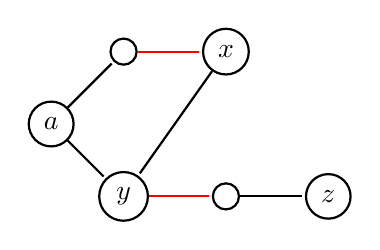
\begin{tikzpicture}[-,>=stealth,shorten >=1pt,auto,node distance=1.3cm, thick,main node/.style={scale=0.9,circle,draw,font=\sffamily\normalsize}]

                \node[circle, draw] (1) []{$a$};
                \node[circle, draw] (2) [above right of = 1]{};
                \node[circle, draw] (3) [right of = 2]{$x$};
                \node[circle, draw] (4) [below right of = 1]{$y$};
                \node[circle, draw] (5) [right of = 4]{};
                \node[circle, draw] (6) [right of = 5]{$z$};

                \draw[-] (1) to (2);
                \draw[-] (2) [red] to (3);
                \draw[-] (1) to (4);
                \draw[-] (4) [red] to (5);
                \draw[-] (5) to (6);
                \draw[-] (3) to (4);

                ;
            \end{tikzpicture}
            % \caption{An example of a perfect matching.}
        \end{figure}

        a possible path for $P$ would be $a \to x \to y \to z$. However, the path $a \to y \to z$ is still an $M$-augmenting path that starts at $a$ but has one fewer edge not in $T$ w.r.t. $P$, contradicting the definition of $P$ $\lightning$.

        Note that, in the general case we would consider the path $P' := a \ T \ y \cup y \ P$, however this is not guaranteed to be a path. The complete proof leverages the fact that $G$ is bipartite in order to prove that $P'$ is indeed a path, but it is very technical and outside the scope of these notes.
    \end{proof}

    Finally, now that we have a procedure which is guaranteed to find an augmenting path in a given bipartite graph, to return a maximum matching it suffices to run the following algorithm.

    \begin{framedalgo}{Maximum matching (bipartite graphs)}
        Given a bipartite graph $G$, the algorithm returns a maximum matching for $G$. \\
        \hrule

        \quad
        \begin{algorithmic}[1]
            \Function{MaximumMatchingBipGraphs}{$G$}
                \State $M := \varnothing$
                \Do
                    \State $P := \textsc{findAugmentingPath}(G)$ \Comment{the previous procedure}
                    \State Swap the edges between $M$ and $E(G) - M$ in $P$
                \doWhile{$P \neq \texttt{None}$}
                \State \textbf{return} $M$
            \EndFunction
        \end{algorithmic}
    \end{framedalgo}

    In particular, the output of this algorithm is guaranteed to be a \tit{maximum} matching thanks to \cref{aug paths}, since the algorithm terminates when there are no more augmenting paths left in the graph $G$.

    \section{Perfect matching}

    By definition, a matching is \tit{not} forced to cover all the vertices of a graph. However, if this happens the matching is called \tbf{perfect matching}.

    \begin{frameddefn}{Perfect matching}
        Given a graph $G$, a \tbf{perfect matching} of $G$ is a matching that covers all the vertices of $G$, i.e. $M$ is a perfect matching if and only if $$\forall v \in V(G) \quad \exists e \in M \quad v \cap e \neq \varnothing$$
    \end{frameddefn}

    \begin{figure}[H]
        \centering
        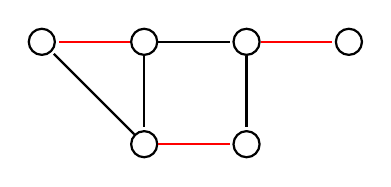
\begin{tikzpicture}[-,>=stealth,shorten >=1pt,auto,node distance=1.3cm, thick,main node/.style={scale=0.9,circle,draw,font=\sffamily\normalsize}]

            \node[circle, draw] (1) []{};
            \node[circle, draw] (2) [right of = 1]{};
            \node[circle, draw] (3) [below of = 1]{};
            \node[circle, draw] (4) [below of = 2]{};
            \node[circle, draw] (5) [left of = 1]{};
            \node[circle, draw] (6) [right of = 2]{};

            \draw[-] (1) to (2);
            \draw[-] (1) to (3);
            \draw[-] (2) to (4);
            \draw[-] (1) [red] to (5);
            \draw[-] (3) [red] to (4);
            \draw[-] (3) to (5);
            \draw[-] (2) [red] to (6);

            ;
        \end{tikzpicture}
        \caption{An example of a perfect matching.}
    \end{figure}

    Perfect matchings are an interesting topic of study when related to \tit{bipartite graphs}. We observe that if a bipartite graph $G$, bipartitioned into $(A, B)$, admits a perfect matching $M$, it must be that $\abs A = \abs B$. This is because every matched edge must connect one vertex from $A$ to one vertex from $B$, and by definition $M$ matched \tit{each} vertex exactly once. However, the converse is not true.

    \begin{figure}[H]
        \centering
        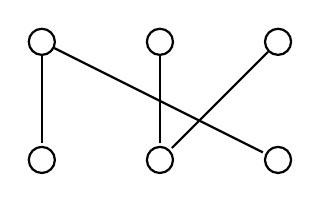
\begin{tikzpicture}[-,>=stealth,shorten >=1pt,auto,node distance=1.5cm, thick,main node/.style={scale=0.9,circle,draw,font=\sffamily\normalsize}]

            \node[circle, draw] (1) []{};
            \node[circle, draw] (2) [right of = 1]{};
            \node[circle, draw] (3) [right of = 2]{};
            \node[circle, draw] (4) [below of = 1]{};
            \node[circle, draw] (5) [below of = 2]{};
            \node[circle, draw] (6) [below of = 3]{};

            \draw[-] (1) to (4);
            \draw[-] (1) to (6);
            \draw[-] (2) to (5);
            \draw[-] (3) to (5);

            ;
        \end{tikzpicture}
        \caption{For instance, this bipartite graph, bipartitioned into $(A, B)$ such that $A$ is the uppermost row of vertices, even if $\abs A = \abs B$ this graph does not admit a perfect matching.}
        % \label{}
    \end{figure}

    \subsection{Hall's theorem}

    Because of this characterization on bipartite graphs, in addition to the concept of \tit{perfect matching}, if $\abs {A} \neq \abs{B}$ we can define a \tit{weaker} version of \curlyquotes{perfect}.

    \begin{frameddefn}{$A$-perfect matching}
        Given a bipartite graph $G$, bipartitioned through $(A, B)$ such that $\abs A \le \abs B$, we say that a matching $M$ is an \tbf{$A$-perfect matching} if it covers all the vertices in $A$.
    \end{frameddefn}

    Note that we can always assume that $\abs A \le \abs B$, without loss of generality. The following theorem, known as the \href{https://en.wikipedia.org/wiki/Hall%27s_marriage_theorem}{Hall's marriage theorem} --- proved by \textcite{hall} in 1935 --- shows the conditions that guarantee that an $A$-perfect matching exists.

        \begin{framedthm}[label={hall}]{Hall's marriage theorem}
        Given a bipartite graph $G$, bipartitioned into $(A, B)$, then $G$ admits an $A$-perfect matching if and only if $$\forall S \subseteq A \quad \abs S \le \abs{\mathcal N (S)}$$
    \end{framedthm}

    \begin{proof}
        The direct implication is trivially true by definition of matching. We will prove the converse implication by contrapositive. Therefore, suppose that the bipartite graph $G$ does not admit any $A$-perfect matching, and consider a minimum vertex cover $V^*$ of $G$. Then, by \cref{konig}, since $G$ is bipartite we know that for any maximum matching $M^*$ of $G$ it holds that $\abs{M^*} = \abs{V^*}$. However, since we are assuming that there are no $A$-perfect matchings of $G$, any maximum matching must have size strictly less than $\abs A$, meaning that $\abs{V^*} = \abs{M^*} < \abs A$.

        Now, consider the set $S := A - V^*$; since $G$ is bipartite, it must hold that $$\mathcal N(S) \subseteq V^* \cap B \implies \abs{\mathcal N(S)} \le \abs{V^* \cap B} = \abs {V^*} - \abs{A \cap V^*}$$ Moreover, observe that $$V^* \cap A = A - (A - V^*) = A - S \implies \abs{V^* \cap A}  = \abs A - \abs S$$ therefore, we have that $$\abs{\mathcal N(S)} \le \abs{V^*} - \abs{V^* \cap A} = \abs{V^*} - \abs A + \abs S$$ Lastly, since $\abs {V^*} < \abs A \iff \abs{V^*} - \abs A < 0$, we conclude that $$\abs{\mathcal N (S)} \le \abs{V^*} - \abs A + \abs S < 0 + \abs S = \abs S \implies \abs{\mathcal N(S)} < \abs S$$ which proves that there is at least one set $S$ for which the \tit{Hall condition} does not hold.
    \end{proof}

    \subsection{Tutte's theorem}

    In the general case, what obstructs the existence of a perfect matching in a graph? Consider a graph $G$; clearly, if $n$ is odd, the graph does not admit perfect matchings, since each edge matches exactly two nodes, meaning that there will always be a free vertex in the graph.

    \begin{figure}[H]
        \centering
        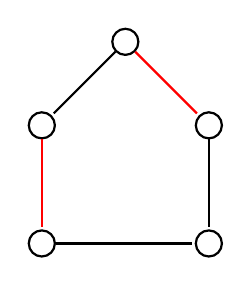
\begin{tikzpicture}[-,>=stealth,shorten >=1pt,auto,node distance=1.5cm, thick,main node/.style={scale=0.9,circle,draw,font=\sffamily\normalsize}]

            \node[circle, draw] (1) []{};
            \node[circle, draw] (2) [below left of = 1]{};
            \node[circle, draw] (3) [below right of = 1]{};
            \node[circle, draw] (4) [below of = 2]{};
            \node[circle, draw] (5) [below of = 3]{};

            \draw[-] (1) to (2);
            \draw[-] (1) [red] to (3);
            \draw[-] (2) [red] to (4);
            \draw[-] (3) to (5);
            \draw[-] (4) to (5);

            ;
        \end{tikzpicture}
        \caption{For instance, no matching of $C_5$ can be perfect.}
    \end{figure}

    For the same reasoning, if $G$ has a connected component with an odd number of vertices, $G$ does not admit perfect matchings. Hence, if $G$ admits a perfect matching, there cannot be any connected component with an odd number of vertices. But is the converse true as well? Consider the following graph

    \begin{figure}[H]
        \centering
        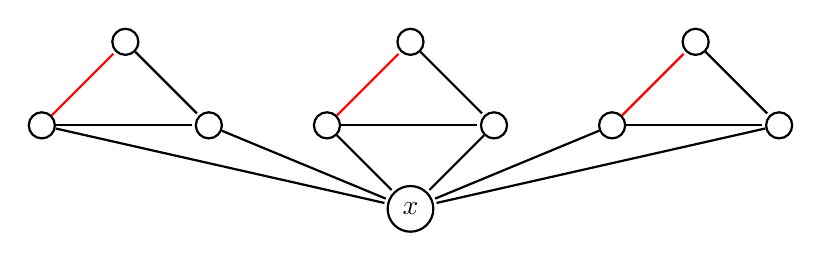
\begin{tikzpicture}[-,>=stealth,shorten >=1pt,auto,node distance=1.5cm, thick,main node/.style={scale=0.9,circle,draw,font=\sffamily\normalsize}]

            \node[circle, draw] (1) []{};
            \node[circle, draw] (2) [above right of = 1]{};
            \node[circle, draw] (3) [below right of = 2]{};
            \node[circle, draw] (4) [right of = 3]{};
            \node[circle, draw] (5) [above right of = 4]{};
            \node[circle, draw] (6) [below right of = 5]{};
            \node[circle, draw] (7) [right of = 6]{};
            \node[circle, draw] (8) [above right of = 7]{};
            \node[circle, draw] (9) [below right of = 8]{};
            \node[circle, draw] (10) [below left of = 6]{$x$};

            \draw[-] (1) [red] to (2);
            \draw[-] (2) to (3);
            \draw[-] (1) to (3);
            \draw[-] (4) [red] to (5);
            \draw[-] (5) to (6);
            \draw[-] (4) to (6);
            \draw[-] (7) [red] to (8);
            \draw[-] (8) to (9);
            \draw[-] (7) to (9);

            \draw[-] (1) to (10);
            \draw[-] (3) to (10);
            \draw[-] (4) to (10);
            \draw[-] (6) to (10);
            \draw[-] (7) to (10);
            \draw[-] (9) to (10);

            ;
        \end{tikzpicture}
        % \caption{For instance, no matching of $C_5$ can be perfect.}
    \end{figure}

    This graph is connected, and has 10 vertices, but it does not admit perfect matchings, meaning that the converse does not hold. Can we find a condition that guarantees that a given graph always admits a perfect matching?

    Given a graph $G$, let $\mathcal O (G)$ be the number of components with an odd number of vertices. The next theorem, proved by \textcite{tutte} in 1947 shows that the following property $$\forall S \subseteq V(G) \quad \mathcal O(G[V(G) - S]) \le \abs S$$ which we will refer to as \tbf{Tutte condition} --- is a \tit{necessary} and \tit{sufficient} condition to guarantee that a graph admits a perfect matching. In fact, in the example of $C_5$ we observe that the set that violates the Tutte condition is $S = \varnothing$, and in the second example is $S = \{x\}$.

    \begin{framedlem}{}
        Given a graph $G$, and a supergraph $G'$ of $G$, if $G$ satisfies the Tutte condition, then $G'$ satisfies the Tutte condition as well.
    \end{framedlem}

    \begin{proof}
        By contrapositive, suppose that $G'$ fails the Tutte condition, meaning that there exists a set $S \subseteq V(G') = V(G)$ such that $\mathcal O (G[V(G') - S]) > \abs S$. Since $G'$ is obtained by adding edges to $G$, the number of odd components in $G'$ can either remain the same, or decrease if two different components having an odd number of vertices became connected in $G'$. Therefore, we have that $$\abs S < \mathcal O (G[V(G') - S]) \le \mathcal O (G[V(G) - S])$$ meaning that $G$ fails the Tutte condition as well.
    \end{proof}

    We are now ready to prove Tutte's theorem.

    \begin{framedthm}{Tutte's theorem}
        A graph $G$ admits a perfect matching if and only if for any $S \subseteq V(G)$ it holds that $\mathcal O(G[V(G) - S]) \le \abs S$ --- meaning that it satisfies the Tutte condition.
    \end{framedthm}

    \proofiff{
        For the direct implication, consider a graph $G$ that admits a perfect matching $M$, and by way of contradiction assume that there exists a set $S \subseteq V(G)$ that violates the Tutte condition. For the previous observation, we know that each component of $G[V(G) - S]$ that has an even number of vertices will not have free nodes w.r.t. $M$, and each component of $G[V(G) - S]$ that has an odd number of vertices will have one free node w.r.t. $M$. In particular, these free vertices must be covered by $M$, since $M$ is perfect, and the only way they can be covered by $M$ is through the vertices of $S$. However, since $\mathcal O (G[V(G) - S]) > \abs S$, there exists at least one free vertex in $G[V(G) - S]$ w.r.t. $M$ that cannot be matched to any of the vertices of $S$, meaning that $M$ is not perfect $\lightning$.
    }{
        We will prove the contrapositive of the converse implication. Therefore, suppose that $G$ does not admit any perfect matching, and we will prove that there exists a set of vertices for which the Tutte condition does not hold. Let $G'$ be the maximal supergraph of $G$ that still does not admit perfect matchings. We say that a set $X$ satisfies the \tit{clique-adjacency} condition if every component of $G'[V(G') - X]$ is a clique, and every vertex $u \in X$ is adjacent to every vertex $v \notin X$.

        \claim{
            If there is a subset $S' \subseteq V(G')$ that satisfies the clique-adjacency condition, then $G$ does not satisfy the Tutte condition.
        }{
            Note that $S' \subseteq V(G') = V(G)$, hence if $S'$ violates the Tutte condition on $G$, the claim is trivially true. Therefore, we will assume that $S'$ satisfies both the clique-adjacency condition, and the Tutte condition on $G$.

            Let $S'$ be a subset that satisfies the clique-adjacency condition; hence, by definition every component of $G'[V(G') - S']$ is a clique. Thus, consider a clique, and let $n$ be the number of its vertices.
            
            \begin{itemize}
                \item If $n$ is even, we can always find a perfect matching restricted on it.
                \item If $n$ is odd, we can always find a perfect matching restricted to $n - 1$ vertices, but since we are assuming that $S'$ satisfies the Tutte condition on $G$, we know that $\mathcal O (G[V(G) - S']) \le \abs {S'}$. Therefore, by the clique-adjacency condition we know that we can always match the $n$-th vertex of the clique with a vertex of $S'$.
            \end{itemize}

            % Note that the free vertices of $S'$ must form a clique as well, otherwise \todo{va visto nel dettaglio il motivo}. 
            TODO \todo{da finire}
        }

        Consider the set $$S := \{v \in V(G') \mid \deg_{G'}(v) = n - 1\}$$ By way of contradiction, suppose that $S$ violates the clique-adjacency condition. This happens if at least one of the following holds:

        \begin{enumerate}[label={(\arabic*)}]
            \item there are two vertices $u \in S$ and $v \notin S$ such that $u \notin S$
            \item there is a component of $G'[V(G') - S]$ that is not a clique
        \end{enumerate}

        However, by definition of $S$, each vertex $v \in S$ has $\deg_{G'} = n - 1$, hence $(1)$ cannot be true, meaning that $(2)$ must hold. Hence, consider a connected component of $G'[V(G') - S]$ that is not a clique, i.e. there are at least two vertices $x$ and $y$ such that $x \nsim y$.

        Let $P$ be the shortest path from $x$ to $y$ in $G'[V(G') - S]$, and let $a$, $b$ and $c$ be the first three vertices of $P$ --- note that $a, b, c \notin S$. We observe that $a \nsim c$, otherwise $P$ would not be the shortest path. Note that $b \notin S$, therefore $\deg_{G'}(b) < n - 1$, i.e. there exists a vertex $d$ such that $b \nsim d$.

        \begin{figure}[H]
            \centering
            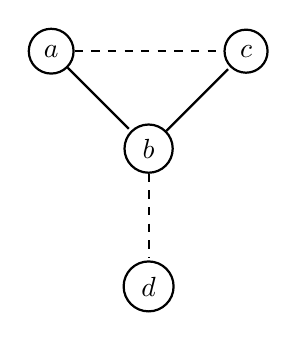
\begin{tikzpicture}[-,>=stealth,shorten >=1pt,auto,node distance=1.75cm, thick,main node/.style={scale=0.9,circle,draw,font=\sffamily\normalsize}]

                \node[circle, draw] (1) []{$a$};
                \node[circle, draw] (2) [below right of = 1]{$b$};
                \node[circle, draw] (3) [above right of = 2]{$c$};
                \node[circle, draw] (4) [below of = 2]{$d$};

                \draw[-] (1) to (2);
                \draw[-] (2) to (3);
                \draw[dashed] (1) to (3);
                \draw[dashed] (2) to (4);

                ;
            \end{tikzpicture}
            \caption{The \curlyquotes{kite-shaped} figure we are considering --- the dashed lines represent the \tit{missing edges}.}
        \end{figure}

        By maximality of $G'$, we know that $G' \cup \{ac\}$ must have a perfect matching $M_1$, and $G' \cup \{bd\}$ must have a perfect matching $M_2$. Moreover, $ac \in M_1$ and $bd \in M_2$, otherwise $M_1$ and $M_2$ would be perfect matchings on $G'$.

        \claim{
            $(M_1 - \{ac\}) \cup (M_2 - \{bd\})$ contains a perfect matching for $G'$.
        }{
            Let $\overline M = (M_1 - \{ac\}) \Delta (M_2 - \{bd\})$. By the same reasoning applied for \cref{aug paths}, since $M_1$ and $M_2$ are two matchings, every vertex of $\overline M$ has degree at most 2. Hence, consider a vertex $z$ in the subgraph induced by $\overline M$

            \begin{itemize}
                \item if $\deg_{\overline M}(z)$ is 0 or 2, $z$ is matched both by $M_1$ and $M_2$
                \item since $M_1$ is a perfect matching, each vertex of $G'$ is matched by $M_1 - \{ac\}$, except for $a$ and $c$
                \item likewise, since $M_2$ is a perfect matching, each vertex of $G'$ is matched by $M_2 - \{bd\}$, except for $b$ and $d$
            \end{itemize}

            which implies that the only vertices $z$ that have $\deg_{\overline M}(z) = 1$ are precisely $a$, $b$, $c$ and $d$.

            Moreover, each component of the subgraph induced by $\overline M$ is either an isolated vertex, a cycle or a path, and the edges of the components must alternate between $M_1$ and $M_2$. Therefore, because of the degrees of $a$, $b$, $c$ and $d$, it must be that these vertices are endpoints of two alternating paths $P_1$ and $P_2$. Moreover, since $ac \in M_1$ and $bd \in M_2$, one of these paths must be an $M_1$-alternating path, while other must be $M_2$ alternating --- and without loss of generality let $P_1$ be the $M_1$-alternating. Note that the set $$M' := (M_1 \cup M_2) - (E(P_1) \cup E(P_2))$$ is a perfect matching on $G[V(G) - (V(P_1) \cup V(P_2))]$. We have three cases for $P_1$ and $P_2$:

            \begin{enumerate}
                \item $P_1$ is a path $a \to c$, and $P_2$ is a path $b \to d$; then $$(M_1 \cap E(P_2)) \cup (M_2 \cap E(P_1)) \cup M'$$ is a perfect matching on $G'$
                \item $P_1$ is a path $a \to b$, and $P_2$ is a path $c \to d$; then $$(M_1 \cap E(P_2)) \cup (M_2 \cap E(P_1)) \cup M' \cup \{bd\}$$ is a perfect matching on $G'$
                \item $P_1$ is a path $a \to d$, and $P_2$ is a path $b \to c$; then $$(M_1 \cap E(P_2)) \cup (M_2 \cap E(P_1)) \cup M' \cup \{ac\}$$ is a perfect matching on $G'$
            \end{enumerate}
        }

        Therefore, because of this claim $G'$ always contains a perfect matching, contradicting the definition of $G'$. This implies that $S$ must satisfy the clique-adjacency condition. Hence, by the first claim we have that $G$ satisfies the Tutte condition \todo{first claim is wrong?}
    }

    \section{Stable matching}

    Matchings in bipartite graphs are particularly useful as they can be applied to model various types of problems across different fields. One well-known example is the \href{https://en.wikipedia.org/wiki/Stable_marriage_problem}{stable matching problem}, which arises in scenarios like job assignments, college admissions, and matchmaking systems. In this problem, the goal is to find a \tit{stable pairing} between two sets of entities --- such as students and universities --- where no two unmatched entities would prefer each other over their current assignments.

    \begin{frameddefn}{Stable matching}
        Given a graph $G$, bipartitioned through $(A, B)$, and a matching $M$ of $G$, consider a family of \tit{preference} functions $\{w_v\}_{v \in V(G)}$ that for each vertex $v \in V(G)$, assign a value to the edges $vu \in E(G)$, for all $u \in \mathcal N (v)$ $$\forall v \in V(G) \quad \func{w_v}{\mathcal N (v)}{\R}$$ We say that $M$ is \tbf{stable} if for each $ab \in E(G)$ it does \underline{not} happen that $$(a \ \mathrm{free} \ \lor (\exists ab' \in M \quad w_a(b) > w_a(b')))$$ $$\land$$ $$(b \ \mathrm{free} \ \lor (\exists a'b \in M \quad w_b(a) > w_b(a')))$$
    \end{frameddefn}

    For instance, consider the following bipartite graph $G$, and a matching $M$ --- outlined in \tit{red}:

    \begin{figure}[H]
        \centering
        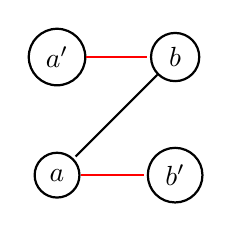
\begin{tikzpicture}[-,>=stealth,shorten >=1pt,auto,node distance=1.5cm, thick,main node/.style={scale=0.9,circle,draw,font=\sffamily\normalsize}]

            \node[circle, draw] (1) []{$a'$};
            \node[circle, draw] (2) [right of = 1]{$b$};
            \node[circle, draw] (3) [below of = 1]{$a$};
            \node[circle, draw] (4) [below of = 2]{$b'$};

            \draw[-] (1) [red] to (2);
            \draw[-] (2) to (3);
            \draw[-] (3) [red] to (4);

            ;
        \end{tikzpicture}
        % \caption{For instance, this bipartite graph, bipartitioned into $(A, B)$ such that $A$ is the uppermost row of vertices, even if $\abs A = \abs B$ this graph does not admit a perfect matching.}
        % \label{}
    \end{figure}

    If the family of preference functions $\{w_v\}_{v \in V}$ is such that $$w_a(b) > w_b(b') \land w_b(a) > w_b(a')$$ which implies that \underline{both} $a$ and $b$ would prefer to \tit{switch} their current matched vertex --- then $M$ is \tit{not} stable. Note that the empty matching is \tit{not} stable, by definition.

    The following theorem, proved by \textcite{gale} in 1962, proves that a stable matching can be always constructed in a bipartite graph, regardless of the preference functions.

    \begin{framedthm}{Gale-Shapley theorem}
        Given a bipartite graph $G$, and a family of preference functions $\{w_v\}_{v \in V(G)}$, there exists a stable matching of $G$.
    \end{framedthm}

    \begin{proof}
        Before proving the theorem, we need to introduce some definitions.

        Consider a bipartite graph $G$, bipartitioned through $(A, B)$, and consider a matching $M$. Given two vertices $a \in A$ and $b \in B$, we say that $a$ is \tbf{acceptable to $b$} if

        \begin{itemize}
            \item $b$ is free, or
            \item $b$ is matched to a vertex $a'$, and $w_b(a) > w_b(a')$
        \end{itemize}

        Moreover, we say that a vertex $a \in A$ is \tbf{happy} if either
        
        \begin{itemize}
            \item $a$ is free, or
            \item $ab \in M$ and for each $b'$ such that $a$ is acceptable to $b'$, it holds that $w_a(b) \ge w_a(b')$
        \end{itemize}

        Observe that in the empty matching every vertex is happy.

        \claim{
            Consider a matching $M$ such that each vertex is happy; if $M$ is not stable, then there exists a vertex $a \in A$ such that $a$ is free and acceptable to some $b \in B$.
        }{
            By instability of $M$, there must be an edge $ab \notin M$ such that $a$ is free, or it prefers $b$ to its current partner, and vice versa. By way of contradiction, suppose that $a$ is matched to some $b' \in B$, hence by instability of $M$ through $ab$ we know that $w_a(b) > w_a(b')$

            \begin{itemize}
                \item If $b$ is free, then by definition $a$ is acceptable to $b$; however, by happiness of $a$ it must be that $w_a(b') \ge w_a(b)$ $\lightning$
                \item If $b$ is matched by some edge $a'b \in M$, by instability of $M$ through $ab$ we know that $w_b(a) > w_b(a')$, hence $a$ is acceptable to $b$, and by happiness of $a$ it must be that $w_a(b') \ge w_a(b)$ $\lightning$
            \end{itemize}

            This implies that $a$ must be free; therefore, we have that

            \begin{itemize}
                \item If $b$ is free as well, then by definition $a$ is acceptable to $b$
                \item If $b$ is matched by some edge $a'b \in M$, by instability of $M$ through $ab$ we know that $w_b(a) > w_b(a')$, hence $a$ is still acceptable to $b$
            \end{itemize}
        }

        Now, consider another matching $M'$ of $G$; we say that $M$ is \tbf{better than $M'$} if 

        \begin{itemize}
            \item $\forall a'b \in M' \quad \exists ab \in M \quad w_b(a) \ge w_b(a')$, meaning that every vertex $b \in B$ prefers its match in $M$ at least as much as its match in $M'$, and
            \item $\exists a'b \in M', ab \in M \quad w_b(a) > w_b(a')$, meaning that there is at least one vertex $b$ that strictly perfers its match in $M$ over its match in $M'$
        \end{itemize}
        
        In other words, $M$ is better than $M'$ if no match in $M$ is worse than in $M'$, and at least one match is strictly better.

        Let $M_k$ be an unstable matching such that every vertex is happy; therefore, by the previous claim we know that there exists a vertex $a \in A$ such that $a$ is free and and acceptable to some $b \in B$. We will construct a matching $M_{k + 1}$ as follows: $$b^* \in \argmax_{\substack{b \in \mathcal N (a) : \\ a \ \mathrm{acceptable \ to} \ b}}{w_a(b)} \implies M_{k + 1} := (M_k \cup \{ab^*\}) - \{a'b^* \in M_k \mid a' \in A\}$$ meaning that $M_{k + 1}$ is obtained from $M_k$ by adding the edge $ab^*$, where $b^*$ maximizes $w_a(b^*)$, and removing the edge $a'b^*$ from $M_k$, if present --- the last set is either $\{a'b^*\}$ or $\varnothing$.

        \claim{
            $M_{k + 1}$ is better than $M_k$, and if $M_k$ is ensures that every vertex is happy, $M_{k +1}$ does as well.
        }{
            First, we prove that $M_{k +1}$ is better than $M_k$. The first condition that $M_{k +1}$ has to satisfy in order to be better than $M_k$ is true simply because we removed the edge $a'b^*$ if it was present in $M_k$, and the rest of the matching has not been altered. Moreover, if $b^*$ was free then the second condition is vacuously true, otherwise if the edge $a'b^*$ was present in $M_k$, in $M_{k +1}$ there we added the edge $ab^*$ and we know that $w_{b^*}(a) > w_{b^*}(a')$ because $a$ is acceptable to $b^*$ by definition.

            Now, assume that $M_k$ is such that every vertex is happy. Since $b^*$ is the neighbor of $a$ that maximizes $w_a(b^*)$, $a$ is happy by definition. Now, if $b^*$ was free in $M_k$, then we only added $ab^*$ to $M_{k + 1}$, hence every vertex is happy w.r.t. $M_{k + 1}$. Otherwise, if $b^*$ was not free in $M_k$, i.e. there was an edge $a'b^* \in M_k$, by definition $M_{k + 1}$ will not contain $a'b^*$, meaning that $a'$ is free w.r.t. $M_{k +1}$, hence $a'$ is happy by definition.
        }

        Now, consider the empty matching $M_0 := \varnothing$; we already observed that $M_0$ is not stable, but is such that each vertex is happy, therefore by the previous claim we can extend $M_0$ into $M_1$ through some vertex $a \in A$ that satisfied the condition of the first claim. In particular, since we proved that this process preserves the happiness of the vertices, we can repeat this process as long as the current matching $M_i$ is still unstable.

        Observe that every matching in the sequence is better than the previous ones, therefore such sequence cannot cycle. Moreover, since there is a finite number of possible matching of $G$, the sequence will eventually reach a matching where every vertex of $A$ is matched --- if $\abs A \neq \abs B$ we can assume that $\abs A < \abs B$ without loss of generality; call this matching $\hat M$. Hence, by contrapositive of the first claim, we know that $\hat M$ is either unstable, or has an unhappy vertex. However, by construction of our sequence, every vertex of $\hat M$ is happy, therefore it must be that $\hat M$ is stable.
    \end{proof}

    \section{Exercises}

    \begin{framedprob}{}
        Let $G$ be a $k$-regular bipartite graph, bipartitioned through $(A, B)$. Prove that

        \begin{enumerate}
            \item $\abs A = \abs B$
            \item $G$ has a perfect matching
        \end{enumerate}
    \end{framedprob}

    \solution{
        Since $G$ is $k$-regular, it holds that the number of edges that have an endpoint in $A$ is precisely $k \abs A$, and the number of edges that have an endpoint in $B$ is exactly $k \abs B$; moreover, since $G$ is bipartite, we have that $$k \abs A = k \abs B \implies \abs A = \abs B$$

        We will prove the second statement by using \cref{hall}. By way of contradiction, assume that there is a set $S \subseteq V(G)$ such that $\abs S > \abs{\mathcal N(S)} \implies k \abs S > k \abs{\mathcal N (S)}$. Applying the same argument as before, the number of edges $ab$ such that $a \in S, b \in \mathcal N (S)$ is exactly $k \abs S$, hence by the pigeonhole principle there must be at least one vertex in $\mathcal N (S)$ that has more than $k$ vertices, contradicting the $k$-regularity of $G$.
    }

    \begin{framedprob}{}
        Let $k$ be an integer. Show that any two partitions of a finite set into $k$-sets admit a common choice of representatives.
    \end{framedprob}

    \solution{
        Let $S$ be a finite set, and let $\mathcal P := \{P_1, \ldots, P_k\}$ and $\mathcal P' : = \{P_1', \ldots, P_k'\}$ be two partitions over $S$ into $k$-sets --- we observe that $\abs{\mathcal P} = \abs{\mathcal P'} = k$ and for any $Q_1, Q_2 \in \mathcal P \cup \mathcal P'$ we have that $\abs{Q_1} = \abs{Q_2} = \tfrac{\abs S}{k}$.

        Now, construct a graph $G$ as follows:
        
        \begin{itemize}
            \item add a vertex for each $k$-set of the two partitions --- hence $V(G) = \mathcal P \cup \mathcal P'$
            \item $\forall Q_1, Q_2 \in \mathcal P \cup \mathcal P' \quad Q_1 \sim Q_2 \iff Q_1 \cap Q_2 \neq \varnothing$
        \end{itemize}

        We observe that $G$ is a bipartite graph, bipartitioned through $(\mathcal P, \mathcal P')$ itself: in fact, since $\mathcal P$ is a partition of $S$, its $k$-sets cannot intersect, hence $\mathcal P$ induces an independent set --- and the same reasoning can be applied for $\mathcal P'$ as well.

        \claim{
            $G$ admits a perfect matching.
        }{
            Fix $X \subseteq \mathcal P$. Since $\mathcal P$ is a partition of $S$ into $k$-sets, we have that $\abs{\bigcup_{P \in X}}{P} = k \abs X$ since the $k$-sets cannot overlap. By a similar argument, since $\mathcal P'$ is a partition of $S$ into $k$-sets as well, we have that $\abs{\bigcup_{P' \in \mathcal N(X)}{P'}} = k \abs{\mathcal N(X)}$.

            By way of contradiction, suppose that there is an element $x \in \bigcup_{P \in X}{P} - \bigcup_{P' \in \mathcal N(X)}{P'}$, meaning that there is an element $x \in P$ for a $k$-set $P \in X$ such that for any $P' \in \mathcal N(X)$ it holds that $x \notin \mathcal P'$. However, $\mathcal P$ and $\mathcal P'$ partition $S$, and in particular they cover $S$, meaning that there exists a $k$-set in $\mathcal P$ containing $x$, say $P'$. Moreover, by construction of $G$ if $x \in P \cap P'$ then $G$ contains the edge $\{P, P'\}$, meaning that $P' \in \mathcal N(X)$, but we assumed that no $k$-set of $\mathcal N(X)$ contained $x$ $\lightning$. This proves that $\bigcup_{P \in X}{P} \subseteq \bigcup_{P' \in \mathcal N(X)}{P'}$.

            Finally, together with the previous observation, this implies that $$k \abs S = \abs{\bigcup_{P \in X}{P}} \le \abs{\bigcup_{P' \in \mathcal N(X)}{P'}} = k \abs{\mathcal N (X)}$$ and in particular, we have that $$k \abs S \le k \abs{\mathcal N(X)} \iff \abs X \le \abs{\mathcal N(X)}$$ meaning that the Hall condition is satisfied for any set $X \subseteq \mathcal P$. Hence, by \cref{hall} we get that $G$ admits a $\mathcal P$-perfect matching, but because $\abs{\mathcal P} = \abs{\mathcal P'}$ then any $\mathcal P$-perfect matching of $G$ is also a perfect matching of $G$.
        }

        Now, let $M$ be a perfect matching of $G$, and consider the set $R$ constructed as follows: for each edge $\{P, P'\} \in M$, pick one element $r \in P \cap P'$ and add it to $R$.

        \claim{
            $R$ is a set of representatives for both $\mathcal P$ and $\mathcal P'$.
        }{
            Since $M$ is a matching, every element of $R$ will represent exactly two partitions, namely one in $\mathcal P$ and the other in $\mathcal P'$. Moreover, since $M$ is perfect, every partition of $\mathcal P$ and $\mathcal P'$ will be covered by at least one element of $R$. Finally, no element of $R$ can represent more than one $k$-set in the same partition since $\mathcal P$ and $\mathcal P'$ are independent sets in $G$.
        }

        This last claim concludes the proof.
    }

    \chapter{Graph packing}

    TODO \todo{introduction}
    
    \begin{frameddefn}{$A$-$B$ paths}
        Given a graph $G$, and two sets $A, B \subseteq V(G)$, an \tbf{$A$-$B$ path} is a path that has one end in $A$, one end in $B$, and no internal vertices in $A \cup B$.
    \end{frameddefn}

    \begin{figure}[H]
        \centering
        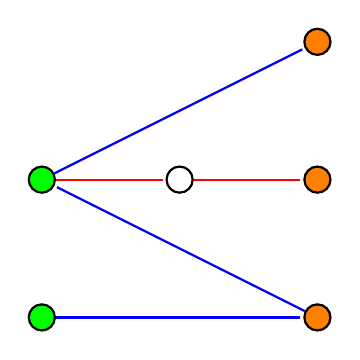
\begin{tikzpicture}[-,>=stealth,shorten >=1pt,auto,node distance=1.75cm, thick,main node/.style={scale=0.9,circle,draw,font=\sffamily\normalsize}]

            \node[circle, draw, fill=green] (1) []{};
            \node[circle, draw] (2) [right of = 1]{};
            \node[circle, draw, fill=orange] (3) [right of = 2]{};
            \node[circle, draw, fill=green] (4) [below of = 1]{};
            \node[circle, draw, fill=orange] (5) [below of = 3]{};
            \node[circle, draw, fill=orange] (6) [above of = 3]{};

            \draw[-] (1) [red] to (2);
            \draw[-] (2) [red] to (3);
            \draw[-] (4) [blue] to (5);
            \draw[-] (5) [blue] to (1);
            \draw[-] (1) [blue] to (6);

            ;
        \end{tikzpicture}
        \caption{For instance, if $A$ is the set of \tit{green} vertices, and $B$ is the set of \tit{orange} vertices, then the \tit{red} is an $A$-$B$ path but the \tit{blue} one is not.}
        % \label{first graph}
    \end{figure}

    Note that if $A \cap B \neq \varnothing$, any vertex in $A \cap B$ is a trivial $A$-$B$ path.

    \begin{frameddefn}{$A$-$B$ hitting set}
        Given a graph $G$, and two sets $A, B \subseteq V(G)$, an \tbf{$A$-$B$ hitting} set is a set $X \subseteq V(G)$ such that every $A$-$B$ path has a vertex in $X$.
    \end{frameddefn}

    \begin{figure}[H]
        \centering
        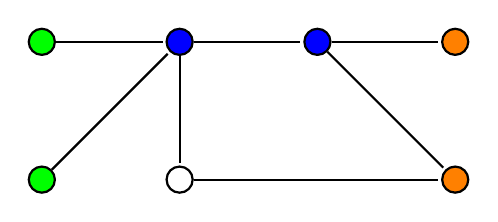
\begin{tikzpicture}[-,>=stealth,shorten >=1pt,auto,node distance=1.75cm, thick,main node/.style={scale=0.9,circle,draw,font=\sffamily\normalsize}]

            \node[circle, draw, fill=green] (1) []{};
            \node[circle, draw, fill=blue] (2) [right of = 1]{};
            \node[circle, draw, fill=blue] (3) [right of = 2]{};
            \node[circle, draw, fill=orange] (4) [right of = 3]{};
            \node[circle, draw] (5) [below of = 2]{};
            \node[circle, draw, fill=green] (6) [below of = 1]{};
            \node[circle, draw, fill=orange] (7) [below of = 4]{};

            \draw[-] (1) to (2);
            \draw[-] (2) to (3);
            \draw[-] (3) to (4);
            \draw[-] (2) to (5);
            \draw[-] (6) to (2);
            \draw[-] (5) to (7);
            \draw[-] (3) to (7);

            ;
        \end{tikzpicture}
        \caption{For example, if $A$ is the set of \tit{green} vertices, and $B$ is the set of \tit{orange} vertices, then the \tit{blue} is an $A$-$B$ hitting set.}
        % \label{first graph}
    \end{figure}

    Note that if $X$ is an $A$-$B$ hitting set, then $A \cap B \subseteq X$, otherwise any single vertex in $A \cap B$ would represent an $A$-$B$ trivial path that does not pass through the hitting set $X$. Moreover, consider an $A$-$B$ hitting set $X$ of a graph $G$; by definition, all the $A$-$B$ paths must have at least one vertex in $X$, but since $A$-$B$ paths do not have internal vertices in $A \cup B$, there cannot be $\abs X + 1$ disjoint $A$-$B$ paths.

    \begin{frameddefn}{$A$-$B$ separation}
        Given a graph $G$, and two sets $A, B \subseteq V(G)$, two sets $X, Y \subseteq V(G)$ describe an $A$-$B$ \tbf{separation $(X, Y)$} of $G$ if and only if

        \begin{itemize}
            \item $A \subseteq X$
            \item $B \subseteq Y$
            \item $X \cup Y = V(G)$
            \item no edge has one end in $X - Y$ and the other in $Y - X$
        \end{itemize}
 
        We say that a separation $(X, Y)$ has \tbf{order} $\abs{X \cap Y}$.
    \end{frameddefn}

    Given a graph $G$, two sets $A, B \subseteq V(G)$, and an $A$-$B$ separation $(X, Y)$ of $G$, we observe that $G[V(G)-(X \cap Y)]$ is disconnected.

    \begin{framedprop}[label={menger prop}]{}
        Given a graph $G$, and two sets $A, B \subseteq V(G)$, there exists an $A$-$B$ hitting set of size $k$ in $G$ if and only if there exists an $A$-$B$ separation of order $k$.
    \end{framedprop}

    \begin{proof}
        The converse implication is trivially true, because if $(X, Y)$ is an $A$-$B$ separation of $G$, then $X \cap Y$ itself is an $A$-$B$ hitting set of $G$ by definition; therefore, we just need to prove the direct implication.
        
        Let $Z$ be an $A$-$B$ hitting set of $G$ such that $\abs Z = k$, and consider the connected components $C_1, \ldots, C_\ell$ of $G[V(G) - Z]$. Note that there cannot be any component $C_i$ that has a vertex $a \in V(G) \cap (A - Z)$ and a vertex $b \in V(C) \cap (B - Z)$, because otherwise by connectivity of $C_i$ there would be a path $a \to b$ --- which is an $A$-$B$ path --- that avoids the hitting set $Z$. Hence, we can define the two following sets $$X := Z \cup \bigcup_{\substack{C \ \mathrm{component} \\ \mathrm{of} \ G[V(G) - Z] \\ \ \mathrm{such \ that} \ A \cap C \neq \varnothing}}{V(C)}$$ $$Y := Z \cup \bigcup_{\substack{C \ \mathrm{component} \\ \mathrm{of} \ G[V(G) - Z] \\ \mathrm{such \ that} \ A \cap C = \varnothing}}{V(C)}$$ We observe that, by definition

        \begin{itemize}
            \item $A \subseteq X$
            \item $Y$ contains all the vertices in $B - Z$, therefore if $B \cap Z = \varnothing$ then trivially $B \subseteq Y$, and if $B \cap Z \neq \varnothing$ we observe that $Z \subseteq Y$ by definition, hence $B$ is always completely covered by $Y$
            \item $X \cap Y = Z$
        \end{itemize}

        and for the previous observation there cannot be edges with one end in $X - Y$ and the other in $Y - X$. Hence, we conclude that $(X, Y)$ is a separation of $G$, and $X \cap Y = Z \implies \abs{X \cap Y} = \abs Z = k$.
    \end{proof}

    The following theorem establishes a deep connection between \tit{connectivity} and \tit{separation} in graphs, and was proved by \textcite{menger} in 1927.

    \begin{framedthm}[label={menger}]{Menger's theorem}
        Given a graph $G$, and two sets $A, B \subseteq V(G)$, the number of disjoint $A$-$B$ paths is equal to the minimum order of an $A$-$B$ separation of $G$.
    \end{framedthm}

    \proofind{
        Consider an $A$-$B$ separation $(X, Y)$ of minimum order of $G$, i.e. a separation that minimizes $\abs{X \cap Y}$; observe that each $A$-$B$ path must traverse at least one vertex of $X \cap Y$, therefore the number of disjoint $A$-$B$ paths that can exist is at most $\abs{X \cap Y}$. This proves the direct implication of the theorem.

        To prove the converse implication, we would need to prove that the minimum order of an $A$-$B$ separation of $G$ is no more than the number of disjoint $A$-$B$ paths. Instead, we will prove that, for a fixed value $k$, in $G$ there are $k$ disjoint $A$-$B$ paths, or there is an $A$-$B$ separation of order at most $k - 1$, which is logically equivalent. In particular, we will proceed by induction on $m$, i.e. the number of edges of $G$.
    }{
        If $m = 0$, the only possible $A$-$B$ paths in $G$ are trivial paths, i.e. isolated vertices in $A \cap B$. Hence, if $\abs{A \cap B} \ge k$ the base case holds; instead, if $\abs{A \cap B} \le k - 1$, we observe that $A \cap B$ itself is an $A$-$B$ hitting set of $G$ of size at most $k - 1$, which means that there exists an $A$-$B$ separation of order at most $k - 1$ by \cref{menger prop}.
    }{
        Assume that the statement holds on a graph that has $m - 1$ edges.
    }{
        We will prove that the statement holds for a graph $G$ that has $m$ edges as well. In particular, fix an edge $xy \in E(G)$, and note that the graph $G - \{xy\}$ has $m - 1$ edges, meaning that the inductive hypothesis holds for $G - \{xy\}$. However, if $G - \{xy\}$ has $k$ disjoint $A$-$B$ paths, then $G$ also has $k$ disjoint $A$-$B$ paths, therefore we may assume that the inductive hypothesis holds for $G - \{xy\}$ precisely because the latter has an $A$-$B$ separation of order at most $k - 1$.

        Hence, let $(X, Y)$ be an $A$-$B$ separation of $G - \{xy\}$ of order at most $k - 1$; we observe that if $x, y \in X$, or $x, y \in Y$, then $(X, Y)$ is also a separation for $G$, which would conclude the proof. Thus, suppose that $x \in X - Y$ and $y \in Y - X$; then $(X, Y \cup \{x\})$ is an $A$-$B$ separation of $G$ that either has still order at most $k - 1$, or it becomes a separation of order $k$ with $k - 1$ $A$-$B$ paths. Since the first case concludes the proof, we may assume the second one to hold.

        Consider the induced subgraphs $G[X]$ and $G[Y]$ \todo{da finire}
    }

    \section{$k$-connectivity}

    \begin{frameddefn}{$k$-connectivity}
        A graph $G$ is said to be \tbf{$k$-connected} if $\abs{V(G)} \ge k + 1$, and for each $X \subseteq V(G)$ such that $\abs X \le k - 1$ it holds that $G[V(G) - X]$ is connected.
    \end{frameddefn}

    In other words, a graph is $k$-connected if it has at least $k + 1$ vertices, and it remains connected whenever fewer than $k$ vertices are removed. Therefor, by definition we observe that if a graph is \tit{not} $k$-connected, it must admit a separation of order at most $k - 1$.

    \begin{figure}[H]
        \centering
        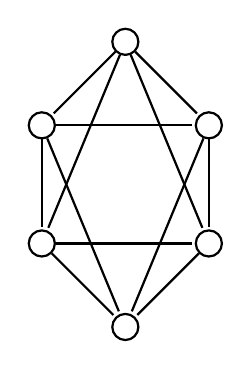
\begin{tikzpicture}[-,>=stealth,shorten >=1pt,auto,node distance=1.5cm, thick,main node/.style={scale=0.9,circle,draw,font=\sffamily\normalsize}]

            \node[circle, draw] (1) []{};
            \node[circle, draw] (2) [below left of = 1]{};
            \node[circle, draw] (3) [below right of = 1]{};
            \node[circle, draw] (4) [below of = 2]{};
            \node[circle, draw] (5) [below of = 3]{};
            \node[circle, draw] (6) [below right of = 4]{};

            \draw[-] (1) to (2);
            \draw[-] (1) to (3);
            \draw[-] (1) to (4);
            \draw[-] (1) to (5);
            \draw[-] (2) to (3);
            \draw[-] (2) to (6);
            \draw[-] (2) to (4);
            \draw[-] (3) to (6);
            \draw[-] (3) to (5);
            \draw[-] (4) to (5);
            \draw[-] (4) to (6);
            \draw[-] (5) to (6);

            ;
        \end{tikzpicture}
        \caption{A 4-connected graph.}
    \end{figure}

    Clearly, any connected graph is 1-connected; moreover, any $K_{t +1}$ clique is $t$-connected.

    \begin{framedprop}[label={kconn}]{}
        If $G$ is $k$-connected, then $\delta \ge k$.
    \end{framedprop}

    \begin{proof}
        By way of contradiction, assume that $\delta < k$, i.e. there is a vertex $x \in V(G)$ such that $\deg(x) < k \implies \abs{\mathcal N(x)} < k$. Now, consider $G[V(G) - \mathcal N (x)]$: this subgraph is disconnected because it has $x$ isolated, but $\abs{\mathcal N(x)} \le k - 1$, meaning that this set contradicts the $k$-connectivity of $G$ $\lightning$.
    \end{proof}

    \begin{framedprop}[label={k-1 conn}]{}
        If $G$ is $k$-connected, then for any $xy \in E(G)$ it holds that $G - \{xy\}$ is $(k - 1)$-connected.
    \end{framedprop}

    \begin{proof}
        By way of contradiction, suppose that $G - \{xy\}$ is not $(k - 1)$-connected, i.e. there exists a set $X \subseteq V(G)$ such that $\abs X \le k - 2$ and $(G - \{xy\})[V(G) - X]$ is disconnected. By $k$-connectivity of $G$, since $\abs X \le k - 2$, we know that $G[V(G) - X]$ is connected, therefore if $(G - \{xy\})[V(G) - X]$ is disconnected it must imply that by removing $xy$ we disconnect $G[V(G) - X]$. Now, since $\abs X \le k - 2$, we know that $\abs{X \cup \{y\}} \le k - 1$, but $G[V(G) - (X \cup \{y\})]$ does not contain the edge $xy$, hence it is disconnected, contradicting the $k$-connectivity of $G$ $\lightning$.
    \end{proof}

    \begin{frameddefn}{Internal disjointness}
        Given a graph $G$, two paths $P_1$ and $P_2$ of $G$ are said to be \tbf{internally disjoint} if every vertex of $V(P_1) \cap V(P_2)$ is an endpoint of $P_1$ and $P_2$.
    \end{frameddefn}

    \begin{figure}[H]
        \centering
        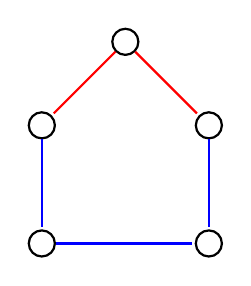
\begin{tikzpicture}[-,>=stealth,shorten >=1pt,auto,node distance=1.5cm,thick,main node/.style={scale=0.9,circle,draw,font=\sffamily\normalsize}]

            \node[circle, draw] (1) []{};
            \node[circle, draw] (2) [below left of = 1]{};
            \node[circle, draw] (3) [below right of = 1]{};
            \node[circle, draw] (4) [below of = 2]{};
            \node[circle, draw] (5) [below of = 3]{};

            \draw[-] (1) [red] to (2);
            \draw[-] (1) [red] to (3);
            \draw[-] (2) [blue] to (4);
            \draw[-] (3) [blue] to (5);
            \draw[-] (4) [blue] to (5);

            ;
        \end{tikzpicture}
        \caption{For instance, the \tit{red} and \tit{blue} paths are internally disjoint.}
    \end{figure}

    \begin{framedprop}{}
        Given a $k$-connected graph, and two sets $A, B \subseteq V(G)$, if $\abs A, \abs B \ge k$ then there exist $k$ disjoint $A$-$B$ paths in $G$.
    \end{framedprop}

    \begin{proof}
        By way of contradiction, if $G$ does not admit $k$ disjoint $A$-$B$ paths, therefore by \cref{menger} the minimum order of an $A$-$B$ separation is at most $k - 1$; hence, let $(X, Y)$ be a minimum order $A$-$B$ separation of $G$, i.e. $\abs{X \cap Y} \le k - 1$. Observe that $\abs{A} \ge k$ and $A \subseteq X$, therefore $\abs X \ge k$ which means that $X - Y \neq \varnothing$, and analogously $Y - X \neq \varnothing$. However, by definition of $A$-$B$ separation we observe that $G[V(G)-(X \cap Y)]$ is disconnected, and we removed less than $k$ vertices, contradicting the $k$-connectivity of $G$ $\lightning$.
    \end{proof}

    \begin{framedthm}[label={intern disj menger}]{}
        A graph is $k$-connected graph if and only if for any pair of vertices $x, y \in V(G)$ such that $x \neq y$ there exist $k$ $\{x\}$-$\{y\}$ internally disjoint paths.
    \end{framedthm}

    \proofiff{
        Fix a pair of distinct vertices $x, y \in V(G)$; we have two cases.

        \begin{itemize}
            \item The two vertices are not adjacent, i.e. $x \nsim y$. By \cref{kconn}, we know that $\abs{\mathcal N(x)} , \abs{\mathcal N(y)} \ge k$, hence by the previous proposition we there exist $k$ disjoint $\mathcal N(x)$-$\mathcal N(y)$ paths, which will form $k$ \tit{internally disjoint} $\{x\}$-$\{y\}$ paths along with the edges to $x$ and $y$.
            \item The two vertices are not adjacent, i.e. $x \nsim y$. By $k$-connectivity of $G$, we know that $G - \{xy\}$ is $(k-1)$-connected by \cref{k-1 conn}, therefore by the same argument of the previous case we have $k - 1$ internally disjoint $\{x\}$-$\{y\}$ path, therefore $G$ will have $k$ internally disjoint $\{x\}$-$\{y\}$ paths along with the edge $xy$.
        \end{itemize}
    }{
        Fix two distinct vertices $x, y \in V(G)$; since there are $k$ $\{x\}$-$\{y\}$ internally disjoint paths, no set of $k - 1$ --- or less --- vertices of $G$ can disconnect $x$ and $y$, implying that $G$ is $k$-connected by definition.
    }

    \begin{framedcor}[label={menger cor}]{}
        Given a $k$-connected graph $G$, a vertex $x \in V(G)$, and a subset $Y \subseteq V(G)$ such that $\abs Y \ge k$, there exist $k$ $\{x\}$-$Y$ paths $P_1, \ldots, P_k$ such that $P_i \cap P_j = \{x\}$ --- for all $i, j \in [k]$ such that $i \neq j$.
    \end{framedcor}

    \begin{proof}
        Add a vertex $z$ to the vertices of $G$, and for each $y \in Y$ add an edge $yz$; we observe that $G[V(G) \cup \{z\}]$ is still $k$-connected, because $\abs Y \ge k$. Now, since $x \neq z$, by the previous proposition there exist $k$ $\{x\}$-$\{z\}$ internally disjoint paths, and these paths must traverse $Y$, therefore each path $P_i$ must have the form $x \to y_i \to z$ for some $y_i \in Y$. Hence, if we consider the subpaths $x \to y_i$ for each $i$, in $G$ these are precisely $k$ $\{x\}$-$Y$ paths intersects only in $x$.
    \end{proof}

    \begin{framedthm}{}
        Given a $k$-connected graph $G$ such that $k \ge 2$, and $k$ vertices $x_1, \ldots, x_k \in V(G)$, there exist a cycle in $G$ that contains all the vertices $x_1, \ldots, x_k$.
    \end{framedthm}
    
    \begin{proof}
        By way of contradiction, let $C$ be the cycle that contains as many vertices $x_i$ as possible; if $x_1, \ldots, x_k \in V(C)$, the theorem is trivially verified, hence we may assume that at least one vertex $x_i$ is not in $V(C)$, and without loss of generality assume that $x_k \notin V(C)$. By \cref{kconn} we know that $\delta \ge k$, and by \cref{min deg 2} we know that $\abs{V(C)} \ge k + 1$. Hence, by the previous corollary we know that exist $k$ $\{x_k\}$-$V(C)$ paths that only intersect in $x_k$.

        Now, since there are at most $k - 1$ vertices $x_i$ in $V(C)$, and there are $k$ $\{x_k\}$-$V(C)$ paths, by the pigeonhole principle there must be a subpath $Q$ of $C$ of the form $x_i \to x_j$ --- for $i, j \in [k - 1]$ distinct --- that has no internal vertex in $\{x_1, \ldots, x_{k - 1}\}$, and such that there are two paths $P_1$ and $P_2$ that $x_k$ as one endpoint and the other lies in $Q$.

        \begin{figure}[H]
            \centering
            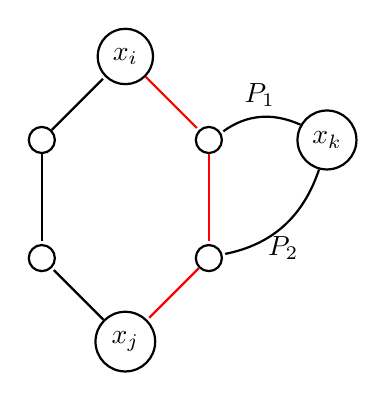
\begin{tikzpicture}[-,>=stealth,shorten >=1pt,auto,node distance=1.5cm,thick,main node/.style={scale=0.9,circle,draw,font=\sffamily\normalsize}]

                \node[circle, draw] (1) []{};
                \node[circle, draw] (2) [above right of = 1]{$x_i$};
                \node[circle, draw] (3) [below right of = 2]{};
                \node[circle, draw] (4) [below of = 3]{};
                \node[circle, draw] (5) [below left of = 4]{$x_j$};
                \node[circle, draw] (6) [above left of = 5]{};
                \node[circle, draw] (7) [right of = 3]{$x_k$};

                \draw[-] (1) to (2);
                \draw[-] (2) [red] to (3);
                \draw[-] (3) [red] to (4);
                \draw[-] (4) [red] to (5);
                \draw[-] (5) to (6);
                \draw[-] (1) to (6);

                \draw[-] (7) [bend right] to node[above]{$P_1$} (3);
                \draw[-] (7) [bend left] to node[below]{$P_2$} (4);

                ;
            \end{tikzpicture}
            \caption{In the figure, the \tit{red} segments compose the subpath $Q$.}
        \end{figure}

        Therefore, we can reroute $Q$ by passing through $P_1$ and $P_2$ in order to find a cycle $C \cup \{x_k\}$ that has a larger number of vertices $x_i$, contradicting the definition of $C$ $\lightning$.
    \end{proof}

    Note that this theorem \tit{does not} guarantee the order in which the vertices are present in the cycle. In fact, asking to preserve the order of the vertices $x_1, \ldots, x_k$ given is a \tit{much harder} question, and the only result we currently know is the following.

    \begin{framedthm}{}
        Given a $10k$-connected graph $G$, and $k$ vertices $x_1, \ldots, x_k \in V(G)$, there exist a cycle in $G$ that contains all the vertices $x_1, \ldots, x_k$ in the same order.
    \end{framedthm}

    \section{Feedback vertex set}

    Consider the following combinatorial structure.

    \begin{frameddefn}{Feedback vertex set}
        Given a graph $G$, a subset $X \subseteq V(G)$ is said to be a \tbf{feedback vertex set} (FVS) if $G[V(G) - X]$ is acyclic; equivalently, $X$ is an FVS if it intersects all cycles of $G$.
    \end{frameddefn}

    \begin{figure}[H]
        \centering
        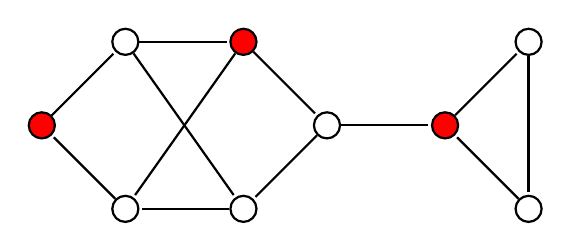
\begin{tikzpicture}[-,>=stealth,shorten >=1pt,auto,node distance=1.5cm,thick,main node/.style={scale=0.9,circle,draw,font=\sffamily\normalsize}]

            \node[circle, draw] (1) []{};
            \node[circle, draw, fill=red] (2) [right of = 1]{};
            \node[circle, draw] (3) [below right of = 2]{};
            \node[circle, draw] (4) [below left of = 3]{};
            \node[circle, draw] (5) [left of = 4]{};
            \node[circle, draw, fill=red] (6) [above left of = 5]{};

            \node[circle, draw, fill=red] (7) [right of = 3]{};
            \node[circle, draw] (8) [above right of = 7]{};
            \node[circle, draw] (9) [below right of = 7]{};

            \draw[-] (1) to (2);
            \draw[-] (2) to (3);
            \draw[-] (3) to (4);
            \draw[-] (4) to (5);
            \draw[-] (5) to (6);
            \draw[-] (6) to (1);

            \draw[-] (3) to (7);
            \draw[-] (7) to (8);
            \draw[-] (8) to (9);
            \draw[-] (9) to (7);

            \draw[-] (1) to (4);
            \draw[-] (2) to (5);

            ;
        \end{tikzpicture}
        \caption{For instance, the \tit{red} set of vertices is an FVS of this graph.}
    \end{figure}

    In many applications, it is important to find a \tbf{minimum} FVS; however, this problem is known to be \NPclass-Complete --- as proved by \textcite{karp} in 1972. Therefore, we often focus on estimating the size of this set by computing lower and upper bounds. In particular, in this section we will present a result proved by \textcite{erdos} in 1965. But before introducing their result about FVSs, we must discuss some combinatorial structures first.

    \subsection{Topological minors}

    Consider a graph $G$, and an edge $xy \in E(G)$; to \tbf{subdivide} $xy$ means to \tit{remove} the edge $xy$ from $E(G)$ and \tit{replacing} it with a 2-edge path $x \ z \ y$ for some new vertex $z$. For instance, if $G$ contains the edge $xy$

    \begin{figure}[H]
        \centering
        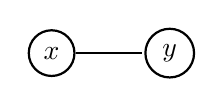
\begin{tikzpicture}[-,>=stealth,shorten >=1pt,auto,node distance=1.5cm,thick,main node/.style={scale=0.9,circle,draw,font=\sffamily\normalsize}]

            \node[circle, draw] (1) []{$x$};
            \node[circle, draw] (2) [right of = 1]{$y$};

            \draw[-] (1) to (2);

            ;
        \end{tikzpicture}
    \end{figure}

    to \tit{subdivide} the edge $xy$ means to replace $xy$ in $G$ with the following 2-edge path

    \begin{figure}[H]
        \centering
        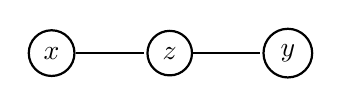
\begin{tikzpicture}[-,>=stealth,shorten >=1pt,auto,node distance=1.5cm,thick,main node/.style={scale=0.9,circle,draw,font=\sffamily\normalsize}]

            \node[circle, draw] (1) []{$x$};
            \node[circle, draw] (2) [right of = 1]{$z$};
            \node[circle, draw] (3) [right of = 2]{$y$};

            \draw[-] (1) to (2);
            \draw[-] (2) to (3);

            ;
        \end{tikzpicture}
    \end{figure}

    \begin{frameddefn}{Subdivision}
        Given a graph $G$, a \tbf{subdivision} of $G$ is a graph obtained from $G$ by repeatedly subdividing its edges.
    \end{frameddefn}

     \begin{figure}[H]
        \centering

        \begin{tabular}{ccc}
            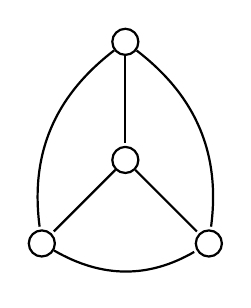
\begin{tikzpicture}[-,>=stealth,shorten >=1pt,auto,node distance=1.5cm,thick,main node/.style={scale=0.9,circle,draw,font=\sffamily\normalsize}]

                \node[circle, draw] (1) []{};
                \node[circle, draw] (2) [below of = 1]{};
                \node[circle, draw] (3) [below left of = 2]{};
                \node[circle, draw] (4) [below right of = 2]{};

                \draw[-] (1) to (2);
                \draw[-] (1) [bend right] to (3);
                \draw[-] (1) [bend left] to (4);
                \draw[-] (2) to (3);
                \draw[-] (2) to (4);
                \draw[-] (3) [bend right] to (4);

                ;
            \end{tikzpicture}

            &\qquad\qquad\qquad&

            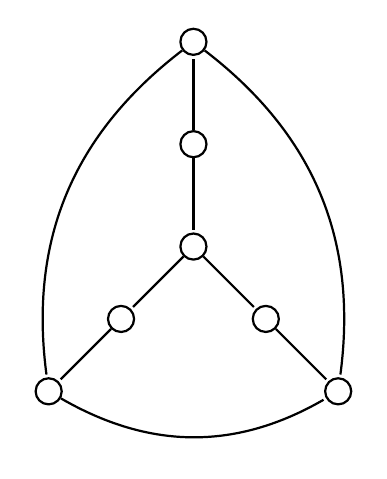
\begin{tikzpicture}[-,>=stealth,shorten >=1pt,auto,node distance=1.3cm, thick,main node/.style={scale=0.9,circle,draw,font=\sffamily\normalsize}]

                \node[circle, draw] (1) []{};
                \node[circle, draw] (2) [below of = 1]{};
                \node[circle, draw] (3) [below left of = 2]{};
                \node[circle, draw] (4) [below right of = 2]{};
                \node[circle, draw] (5) [above of = 1]{};
                \node[circle, draw] (6) [below left of = 3]{};
                \node[circle, draw] (7) [below right of = 4]{};

                \draw[-] (1) to (2);
                \draw[-] (5) [bend right] to (6);
                \draw[-] (5) [bend left] to (7);
                \draw[-] (2) to (3);
                \draw[-] (2) to (4);
                \draw[-] (1) to (5);
                \draw[-] (3) to (6);
                \draw[-] (4) to (7);
                \draw[-] (6) [bend right] to (7);

                ;
            \end{tikzpicture}
        \end{tabular}

        \caption{On the left: $K_4$. On the right: a subdivision of $K_4$.}
    \end{figure}

    Trivially, any graph is a subdivision of itself.

    \begin{frameddefn}{Topological minor}
        Given a graph $G$, and a graph $H$, we say that $G$ contains $H$ as \tbf{topological minor} if $G$ has a subgraph which is a subdivision of $H$. Similarly, we say that $H$ is a \tit{topological minor} of $G$.
    \end{frameddefn}

    \begin{figure}[H]
        \centering
        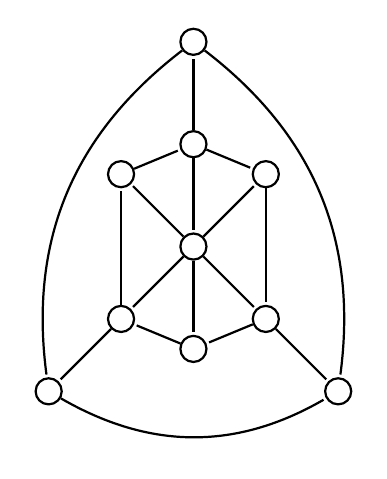
\begin{tikzpicture}[-,>=stealth,shorten >=1pt,auto,node distance=1.3cm, thick,main node/.style={scale=0.9,circle,draw,font=\sffamily\normalsize}]

            \node[circle, draw] (1) []{};
            \node[circle, draw] (2) [below of = 1]{};
            \node[circle, draw] (3) [below left of = 2]{};
            \node[circle, draw] (4) [below right of = 2]{};
            \node[circle, draw] (5) [above of = 1]{};
            \node[circle, draw] (6) [below left of = 3]{};
            \node[circle, draw] (7) [below right of = 4]{};
            \node[circle, draw] (8) [above left of = 2]{};
            \node[circle, draw] (9) [above right of = 2]{};
            \node[circle, draw] (10) [below of = 2]{};

            \draw[-] (1) to (2);
            \draw[-] (5) [bend right] to (6);
            \draw[-] (5) [bend left] to (7);
            \draw[-] (2) to (3);
            \draw[-] (2) to (4);
            \draw[-] (1) to (5);
            \draw[-] (3) to (6);
            \draw[-] (4) to (7);
            \draw[-] (6) [bend right] to (7);
            \draw[-] (2) to (8);
            \draw[-] (2) to (9);
            \draw[-] (2) to (10);

            \draw[-] (8) to (1);
            \draw[-] (1) to (9);
            \draw[-] (9) to (4);
            \draw[-] (4) to (10);
            \draw[-] (10) to (3);
            \draw[-] (3) to (8);

            ;
        \end{tikzpicture}
        \caption{For instance, this graph has $K_4$ as topological minor, because it contains a subdivision of $K_4$ as subgraph.}
    \end{figure}

    \begin{framedprop}[label={3-conn prop}]{}
        If $G$ is 3-connected, then $G$ has $K_4$ as topological minor.
    \end{framedprop}

    \begin{proof}
        If $G$ is 3-connected, then by \cref{kconn} we know that $\delta(G) \ge 3$, and by \cref{min deg 2} this means that in $G$ there is a cycle $C$. Moreover, by 3-connectivity of $G$, we know that $G$ cannot be a cycle itself, therefore there must be at least one vertex $v \notin V(C)$. Now, by 3-connectivity agin we can apply \cref{menger cor}, obtaining 3 $\{v\}$-$V(C')$ paths $P_1$, $P_2$ and $P_3$ that only intersect in $v$, and finally $G[V(C) \cup V(P_1) \cup V(P_2) \cup V(P_3)]$ is a subdivision of $K_4$.
    \end{proof}

    \subsection{Erdős-Pósa theorem}

    \begin{framedprop}{}
        If $G$ is 3-regular multigraph, then $G$ has a cycle of length at most $2 \ceil{\log n}$.
    \end{framedprop}

    \begin{proof}
        Clearly, if $G$ admits loops or parallel edges, the statement is trivially true, therefore we may assume that $G$ is a simple graph.

        Fix a vertex $v \in V(G)$, and grow a BFS tree $T$ from $x$ as long no cycles of length at most $2 \ceil{\log n}$ are encountered. Since $G$ is 3-regular, $T$ will be a tree in which the root $x$ has 3 children, and all the other nodes that are not leaves will have 2 children. If the BFS stopped before visiting all the vertices of $G$, the statement holds, so we may assume that $T$ covers all $V(G)$.

        By 3-regularity of $G$, we have that

        \begin{itemize}
            \item $\delta \ge 3$, hence by \cref{min deg 2} we know that $G$ must contain a cycle
            \item the only possible cycle that can be formed in $G$ is by connecting two leaves of $T$ through an edge
        \end{itemize}

        and lastly, since $V(T) = V(G) = n$, the height of $T$ is $\ceil{\log n} - 1$, which means that such a cycle must have length $$\ceil{\log n} - 1 + \ceil{\log n} - 1 + 1 = 2 \ceil{\log n} - 1$$
    \end{proof}

    Along with the \tit{subdivision} operation that we introduced previously, it naturally follows to defined the \tit{inverse} operation of the subdivision, i.e. the \tbf{suppression}. Given a graph $G$, and two edges $xz, zy \in E(G)$ such that $\deg(z) = 2$, to \tit{suppress} $z$ means to \tit{remove} the vertex $z$ from $V(G)$ along with the edges $xz$ and $zy$, and \tit{replacing} them with an edge $xy$ in $E(G)$. For instance, if $G$ contains the edges $xz$ and $zy$

    \begin{figure}[H]
        \centering
        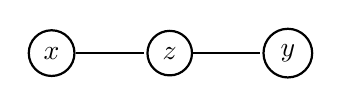
\begin{tikzpicture}[-,>=stealth,shorten >=1pt,auto,node distance=1.5cm,thick,main node/.style={scale=0.9,circle,draw,font=\sffamily\normalsize}]

            \node[circle, draw] (1) []{$x$};
            \node[circle, draw] (2) [right of = 1]{$z$};
            \node[circle, draw] (3) [right of = 2]{$y$};

            \draw[-] (1) to (2);
            \draw[-] (2) to (3);

            ;
        \end{tikzpicture}
    \end{figure}

    to \tit{suppress} the vertex $z$ means to replace $xz$ and $zy$ in $G$ with the following edge $xy$

    \begin{figure}[H]
        \centering
        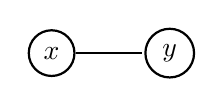
\begin{tikzpicture}[-,>=stealth,shorten >=1pt,auto,node distance=1.5cm,thick,main node/.style={scale=0.9,circle,draw,font=\sffamily\normalsize}]

            \node[circle, draw] (1) []{$x$};
            \node[circle, draw] (2) [right of = 1]{$y$};

            \draw[-] (1) to (2);

            ;
        \end{tikzpicture}
    \end{figure}

    Now, consider the following definition.

    \begin{frameddefn}{Cut}
        Given an undirected graph $G = (V, E)$, and two subsets $S, T \subseteq V$, the \tbf{cut} induced by $S$ and $T$ on $G$ is defined as follows $$\mathrm{cut}(S, T) = \{e \in E : \abs{S \cap e} = \abs{T \cap e} = 1\}$$ In the case in which $T = \overline S = V - S$ we will simply write $\mathrm{cut}(S) = \mathrm{cut}(S, \overline S)$.
    \end{frameddefn}

    In other words, a \tit{cut} induced by a two sets $S$ and $T$ of vertices is the set of edges that have one endpoint in $S$ and the other one in $T$.

    \begin{figure}[H]
        \centering
        \begin{tikzpicture}[-,>=stealth,shorten >=1pt,auto,node distance=1.5cm,thick,main node/.style={scale=0.9,circle,draw,font=\sffamily\normalsize}]

            \node[circle, draw] (1) []{};
            \node[circle, draw, fill=red] (2) [right of = 1]{};
            \node[circle, draw] (3) [below of = 1]{};
            \node[circle, draw, fill=red] (4) [right of = 3]{};
            \node[circle, draw] (5) [left of = 1]{};

            \draw[-] (1) [green] to (2);
            \draw[-] (2) to (4);
            \draw[-] (1) to (3);
            \draw[-] (3) [green] to (4);
            \draw[-] (1) to (5);
            \draw[-] (3) to (5);

            ;
        \end{tikzpicture}
        \caption{For instance, if the set $S$ is described by the \tit{red} vertices, then $\mathrm{cut}(S)$ is the set of green edges.}
    \end{figure}

    We will use the definition of cut in order to prove the following lemma.

    \begin{framedlem}{}
        Given a 3-regular graph $H$ such that $\abs{V(H)} \ge c'k \log (k +1)$ for some constant $c'$, then $H$ contains $k$ disjoint cycles.
    \end{framedlem}

    \proofind{
        We proceed by induction on $k$.
    }{
        For $k = 1$, if $H$ is 3-regular then $\delta(H) = 3$, therefore by \cref{min deg 2} it must contain a cycle.
    }{
        Assume that the statement holds for $k - 1$.
    }{
        Let $C$ be a cycle of $H$, and consider the graph $H - E(C)$.

        \claim{
            $H - E(C)$ has a 3-regular graph $H'$ as topological minor, such that $\abs{V(H')} \ge \abs{V(H)}- 2\abs{V(C)}$.
        }{
            Starting with $V := V(C)$, as long as $H - V$ contains vertices of degree at most 1, move them into $V$; let $M$ be the number of moved vertices. Then, since we are adding vertices to $V$, we have that $\abs{\mathrm{cut}(V)} \le \abs{\mathrm{cut}(C)} - M$. We observe that, by construction $\delta(H - V) \ge 2$, and the number of vertices that have degree 2 in $H - V$ is at most $\abs{\mathrm{cut}(V)} \le \abs{\mathrm{cut}(C)} - M$.

            Lastly, let $H'$ be the graph obtained from $H - V$ by suppressing all the vertices of degree 2; then we have that $H'$ contains at least the vertices of $H$, without the vertices of $C$, the $M$ vertices that we moved during the procedure, and the vertices of degree 2 that we suppressed. In other words, we have that $$\abs{V(H')} \ge \abs{V(H)} - \abs{V(C)} - M - (\abs{\mathrm{cut}(C)}-M) \ge \abs{V(H)} - 2\abs{V(C)}$$ Note that the last inquality comes from the observation that $\abs{\mathrm{cut}(C)} \le \abs{V(C)}$, which follows by 3-regularity of $H$

            Finally, since $H'$ is 3-regular by construction, and $H - V$ is a subdivision of $H'$ that is contained in $H - E(C)$, this concludes the claim.
        }

        Now, since $\abs{V(H)} \ge c'k \log(k + 1)$, and by the previous proposition we know that $$\abs{V(C)} \le 2 \log (\abs{V(H)}) + 2 \iff - 2 \abs{V(C)} \ge - 4 \log (\abs{V(H)}) - 4$$ where the added term 2 takes care of the rounding error from the ceiling operation --- we obtain the following
        \begin{equation*}
            \begin{split}
                \abs{V(H')} &\ge \abs{V(H)} - 2\abs{V(C)} \\
                            &\ge \abs{V(H)} - 4 \log (\log{V(H)}) - 4 \\
                            &\ge c'k \log (k +1) - 4 \log (c'k \log (k + 1)) - 4 \\
                            &\ge c'k \log (k + 1) - 4[ \log c' + \log k + \log(\log(k + 1))] - 4
            \end{split}
        \end{equation*}

        which is at least $c'(k - 1) \log k$ for sufficiently big values of $c'$. In particular, since $\abs{V(H')} \ge c' (k - 1) \log k$, and we know that $H'$ is 3-regular, we can apply the inductive hypothesis on $H'$, which means that $H'$ contains $k - 1$ disjoint cycles.

        Finally, if $H'$ contains $k$ disjoint cycles, and $H - E(C)$ has $H'$ as topological minor, i.e. $H - E(C)$ contains a subdivision $H''$ of $H'$, by definition of the subdivision operation $H''$ will contain $k -1$ disjoint cycles as well. Therefore, since $H - E(C)$ contains $H''$, $H$ contains $k$ disjoint cycles along with the cycle $C$.
    }

    We are now ready to prove the theorem that we introduced at the beginning of this section.

    \begin{framedthm}{Erdős-Pósa theorem}
        There is a constant $c$ such that for any graph $G$, and any $k \in \N$

        \begin{itemize}
            \item either $G$ has $k$ vertex-disjoint cycles or
            \item there is an FVS $X$ of $G$ such that $\abs X \le c k\log k$
        \end{itemize}
    \end{framedthm}

    \begin{proof}
        If $G$ contains $k$ disjoint cycles, the theorem is trivially true, hence we may assume that $G$ does not have $k$ disjoint cycles. Fix $H$ to be the larget subgraph of $G$ such that $\forall v \in V(H) \quad 2 \le \deg_H(v) \le 3$ --- note that $H$ always exists because we may assume that $G$ contains at least 1 cycle, since if $G$ is acyclic the theorem is trivially true (and we would pick the cycle as $H$ itself). Moreover, fix $\overline H$ to be the subgraph of $G$ without all the \curlyquotes{cycle components} of $G$ --- i.e. components of $G$ that are cycles --- and let $U := \{v \in V(\overline H) \mid \deg_{\overline H}(v) = 3\}$.

        By TODO \todo{discrepanze lemma} we know that $\abs{U} < c'k\log(k + 1)$, for some constant $c$. Let $W$ be a set of vertices composed of one vertex for each cycle component --- the ones not present in $\overline H$.

        \claim{
            Every cycle of $G$ is in $H$.
        }{
            If there was a cycle of $G$ not present in $H$, this cycle would have contained vertices of degree at least 2, contradicting the maximality of $H$.
        }

        \tbf{Claim:} There are no paths $P$ in $G[V(G) - (U \cup W)]$ of length at least 1 such that

        \begin{itemize}
            \item both ends of $P$ are in $H[V(H) - (U \cup W)]$
            \item no internal vertex of $P$ is in $H$
            \item no edge of $P$ is in $H$
        \end{itemize}

        \proofenv[Proof of the Claim]{
            If such a path $P$ exists, then $H \cup P$ is a bigger graph than $H$ that has every vertex of degree 2 or 3, contradicting the maximality of $H$.
        }

        \claim{
            Every cycle of $G - (U \cup W)$ intersects $H$ in exactly one vertex.
        }{
            TODO \todo{da finire}
        }

        TODO \todo{da finire}
    \end{proof}

    \section{Directed graphs}

    Up until this point, we only discussed \tit{undirected graphs}. In this section we are going briefly presents some results regarding \tbf{directed graphs} (or \tit{digraphs}, for short), in which the edges have an \tbf{orientation} --- implying that the edge $(x, y)$ is different from the edge $(y, x)$.

    \begin{figure}[H]
        \centering
        \begin{tikzpicture}[-,>=stealth,shorten >=1pt,auto,node distance=1.75cm, thick,main node/.style={scale=0.9,circle,draw,font=\sffamily\normalsize}]

            \node[circle, draw] (1) []{1};
            \node[circle, draw] (2) [right of = 1]{2};
            \node[circle, draw] (3) [below left of = 1]{3};
            \node[circle, draw] (4) [below right of = 2]{4};
            \node[circle, draw] (5) [below right of = 3]{5};
            \node[circle, draw] (6) [below left of = 4]{6};

            \draw[->] (1) [bend left] to (3);
            \draw[->] (1) to (4);
            \draw[->] (1) to (6);
            \draw[->] (2) to (4);
            \draw[->] (2) to (5);
            \draw[->] (3) [bend left] to (1);
            \draw[->] (3) to (5);
            \draw[->] (3) to (6);
            \draw[->] (5) to (6);
            \draw[->] (6) [bend left] to (5);

            ;
        \end{tikzpicture}
        \caption{An example of a \tit{digraph}.}
    \end{figure}

    \begin{frameddefn}{Path cover}
        Let $G$ be a digraph; a \tbf{path cover} for $G$ is a set $\mathcal P$ of disjoint paths such that $$\displaystyle V(G) = \bigcup_{P \in \mathcal P}{V(P)}$$
    \end{frameddefn}

    \begin{figure}[H]
        \centering
        \begin{tikzpicture}[-,>=stealth,shorten >=1pt,auto,node distance=1.75cm, thick,main node/.style={scale=0.9,circle,draw,font=\sffamily\normalsize}]

            \node[circle, draw] (1) []{1};
            \node[circle, draw] (2) [right of = 1]{2};
            \node[circle, draw] (3) [below left of = 1]{3};
            \node[circle, draw] (4) [below right of = 2]{4};
            \node[circle, draw] (5) [below right of = 3]{5};
            \node[circle, draw] (6) [below left of = 4]{6};

            \draw[->] (1) [bend left, red] to (3);
            \draw[->] (1) to (4);
            \draw[->] (1) to (6);
            \draw[->] (2) [red] to (4);
            \draw[->] (2) to (5);
            \draw[->] (3) [bend left] to (1);
            \draw[->] (3) [red] to (5);
            \draw[->] (3) to (6);
            \draw[->] (5) [red] to (6);
            \draw[->] (6) [bend left] to (5);

            ;
        \end{tikzpicture}
        \caption{For instance, if we consider the digraph of the previous example, the set of \tit{red} vertices form a \tit{path cover}.}
        \label{path cover}
    \end{figure}

    We observe that any digraph contains a trivial path cover, i.e. the one formed by the sef of every trivial path of the graph. In fact, we are interested in finding the path cover having \tit{minimum cardinality}. \textcite{gallai} proved that path covers are strictly related to independent sets, through the following theorem.

    \begin{framedthm}{Gallai-Milgram theorem}
        Given a digraph $G$, there are a path cover $\mathcal P$ of $G$ and an independent set $X \subseteq V(G)$ such that $$\forall P \in \mathcal P \quad \abs{X \cap V(P)} = 1$$
    \end{framedthm}

    We are going to prove a slightly stronger result that directly implies the above theorem. First, consider the following definitions.

    \begin{frameddefn}{Terminal nodes}
        Given a digraph $G$, and a path cover $\mathcal P$ of $G$, the set of \tbf{terminal nodes} of the paths of $\mathcal P$ is defined as follows: $$\mathrm{ter}(\mathcal P) := \{v \in V(P) \mid P \in \mathcal P \land \deg_P^{out}(v) = 0\}$$
    \end{frameddefn}

    For example, in \cref{path cover} the terminal nodes are 4 and 6.

    \begin{frameddefn}{Minimality by inclusion}
        Given a digraph $G$, and a path cover $\mathcal P$ of $G$, we say that $\mathcal P$ is \tbf{minimal by inclusion} if there is no other path cover $\mathcal P'$ of $G$ such that $\mathrm{ter}(\mathcal P') \subset \mathrm{ter}(\mathcal P)$.
    \end{frameddefn}

    For instance, the path cover $\mathcal P$ in \cref{path cover} is clearly minimal by inclusion, because no directed edge can be removed from $\mathcal P$ such that the latter still covers $G$.

    \begin{framedprop}{}
        Given a graph $G$, and a path cover $\mathcal P$ of $G$ that is minimal by inclusion, there is an independent set $X \subseteq V(G)$ such that $$\forall P \in \mathcal P \quad \abs{X \cap V(P)} = 1$$
    \end{framedprop}

    \begin{proof}
        TODO \todo{da fare}
    \end{proof}

    \section{Exercises}
    
    \begin{framedprob}{}
        Given a $k$-connected graph $G$ such that $\abs{V(G)} \ge 2k$, show that $G$ contains a cycle of length at least $2k$.
    \end{framedprob}

    \solution{
        Since $\abs{V(G)} \ge 2k$, we can split $G$ into two sets $A$ and $B$ such that $\abs{A}, \abs{B} \ge k$ and $A \cap B = \varnothing$. Fix a vertex $a \in A$; since $G$ is $k$-connected and $\abs A \ge k$, by \cref{menger cor} there exists at least one $\{a\}$-$B$ path, and let $b \in B$ be the other endpoint of this path. By the same argument, since $\abs B \ge k$ there exists at least one $\{b\}-A$ path different from $a \to b$, and let $a' \in A$ be the other endpoint of this path.

        We can repeat the same argument --- starting from $a'$ --- going \curlyquotes{back and forth} from $A$ to $B$, and since $\abs A , \abs B \ge k$ this process can be repeated at least $2k - 1$ times. Hence, at the end of this procedure we found a path $P$ such that $\abs{E(P)} \ge 2k - 1$ that starts in $a$ and ends in some vertex $x \in B$.

        Lastly, consider the vertices $a$ and $x$; clearly $a \neq x$, and since $G$ is $k$-connected by \cref{intern disj menger} there exists at least one $\{x\}$-$\{a\}$ path $P_{x,a}$, meaning that $P \cup P_{x,a}$ forms a cycle in $G$ that must have length at least $2k - 1 + 1 = 2k$.
   }

    \begin{framedprob}{}
        Prove that any $t$-connected subgraph $G$ with $n \ge t + 2$ contains $K_{2, t}$ as a topological minor.
    \end{framedprob}

    \solution{
        Fix two vertices $x , y \in V(G)$; since $n \ge t + 2$, we have that $\abs{V(G) - \{x, y\}} \ge t$, and since $G$ is $t$-connected, by \cref{menger cor}
        
        \begin{itemize}
            \item there are $t$ $\{x\}$-$V(G) - \{x, y\}$ paths that only intersect in $x$ --- let $X$ be the set of the first vertices that these paths encounter from $x$ to $V(G) - \{x, y\}$
            \item there are $t$ $\{y\}$-$V(G) - \{x, y\}$ paths that only intersect in $y$ --- let $Y$ be the set of the first vertices that these paths encounter from $y$ to $V(G) - \{x, y\}$
        \end{itemize}

        and in particular, we observe that $\abs X, \abs Y \ge t$.

        Fix two vertices $a \in X$ and $b \in Y$; by \cref{intern disj menger}, $a$ and $b$ must be connected by at least one path, say $P_{b, a}$. Now, if we consider the path $P_{y, b}$ that connects $y$ and $a$, we get a path $P_{y, b} \cup P_{b, a}$ that connects $y$ and $a$.

        The same reasoning can be applied to any pair of vertices in $X$ and $Y$, which means that all the vertices in $X$ are connected to $x$ by definition, and they are also connected to $y$ thanks to the paths passing through $Y$. This implies that $G$ contains a subgraph that is a subdivision of $K_{2, t}$, meaning that $K_{2, t}$ is a topological minor of $G$.
    }

    \begin{framedprob}{}
        Show, without using Menger's theorem, that any two vertices of a 2-connected graph lie on a common cycle.
    \end{framedprob}
    
    \solution{
        Let $G$ be a 2-connected graph, and by way of contradiction suppose that there are two vertices $x, y \in V(G)$ that do not lie on a common cycle of $G$. By \cref{kconn}, we know that $\delta \ge 2$, hence there must be vertices $x_1, x_2$ and $y_1, y_2$ such that $x \sim x_1, x_2$ and $y \sim y_1, y_2$.

        If $x$ and $y$ do not lie on a common cycle, without of loss of generality we may assume that $x_1$ and $y_1$ are connected by only one path --- there must be at least one otherwise $G$ would be disconnected. However, since $x_1 \sim x \sim x_2$ and $y_1 \sim y \sim y_2$, such path must pass through $x$, $x_2$, $y_2$ and $y$. In particular, this implies that $G - \{x_2\}$ is disconnected because $x_1$ and $y_1$ are not connected anymore. Therefore, we can find a set of 1 vertex that disconnects $G$, meaning that $G$ is not 2-connected $\lightning$.
    }
    
    \begin{framedprob}{}
        Solve the following exercises on $k$-connectivity.

        \begin{itemize}
            \item Give an example of a 2-connected graph $G$ such that for any $C \subseteq G$ it holds that $G - C$ is disconnected.
            \item Prove that every 3-connected graph $G$ has a cycle $C$ such that $G - C$ is connected.
        \end{itemize}
    \end{framedprob}
    
    \solution{
        For the first exercise, a minimal example is given by the following graph:

        \begin{figure}[H]
            \centering
            \begin{tikzpicture}[-,>=stealth,shorten >=1pt,auto,node distance=1.75cm, thick,main node/.style={scale=0.9,circle,draw,font=\sffamily\normalsize}]

                \node[circle, draw] (1) []{};
                \node[circle, draw] (2) [below left of = 1]{};
                \node[circle, draw] (3) [below right of = 1]{};
                \node[circle, draw] (4) [below right of = 2]{};
                \node[circle, draw] (5) [left of = 2]{};
                \node[circle, draw] (6) [right of = 3]{};

                \draw[-] (1) to (2);
                \draw[-] (1) to (3);
                \draw[-] (1) [bend right] to (5);
                \draw[-] (1) [bend left] to (6);
                \draw[-] (2) to (4);
                \draw[-] (3) to (4);
                \draw[-] (4) [bend left] to (5);
                \draw[-] (4) [bend right] to (6);

                ;
            \end{tikzpicture}
        \end{figure}

        TODO \todo{da finire}
    }

    \begin{framedprob}{}
        Prove that every 3-connected graph has a cycle of even length.
    \end{framedprob}

    \solution{
        Consider a 3-connected graph $G$, and by way of contradiction suppose that $G$ has no even length cycles. Fix two adjacent vertices $u, v \in V(G)$; by \cref{intern disj menger} we know that there are at least 3 $\{u\}$-$\{v\}$ paths in $G$, and since the edge $\{u, v\}$ is already a path, we may assume there are at least two other internally disjoint paths $P_1$ and $P_2$ that have $u$ and $v$ as endpoints.

        However, observe that $P_1 \cup \{u, v\}$ and $P_2 \cup \{u, v\}$ are cycles, therefore they must have odd length for the sake of contradiction --- say that $2k + 1$ and $2h + 1$ are the length of the first and the second cycle, respectively. Then, consider $P_1 \cup P_2$: since $P_1$ and $P_2$ are internally disjoint, this is another cycle of $G$, that has length $$(2k + 1) - 1 + (2h + 1) - 1 = 2k + 2h - 2$$ which is even, contradicting the fact that $G$ only had odd-length cycles $\lightning$.
    }

    \chapter{Extremal graph theory}

    Extremal graph theory is a field of mathematics that investigates how \tit{global properties} of a graph influence the \tbf{presence or absence} of specific substructures. Broadly speaking, it seeks to understand how large or dense a graph can be while avoiding certain configurations, or conversely, what constraints guarantee the appearance of particular patterns.

    The central theme of the discipline lies in \tit{exploring thresholds}: determining the minimal or maximal values of graph parameters --- such as the number of edges, degrees, or vertices --- beyond which a given substructure must necessarily exist. These substructures can range from simple motifs like \tit{paths} and \tit{cycles} to more complex or irregular patterns.

    This area plays a crucial role in understanding the fundamental behavior of graphs under constraints, offering insights that are both theoretically significant and applicable in various areas such as network design, data analysis, and algorithm optimization.

    \section{Edge bounds}

    In the first section of this chapter, we will explore the bounds on the number of \tbf{edges} that force any graph to contain interesting substructures. In particular, we define $\mathrm{ex}(n, H)$ to be the minimum number of edges in an $n$-vertex graph that guarantees the existence of $H$ as subgraph.

    \subsection{Cliques}

    We will start our discussion of extremal graph theory with the question of \tbf{determining the existence} of cliques within a given graph. In general, finding the largest clique in a graph is an \NPclass-Hard problem. This leads to a natural question: under what conditions can we guarantee the existence of a $K_n$ subgraph?

    \href{https://en.wikipedia.org/wiki/P%C3%A1l_Tur%C3%A1n}{Pál Turán} addressed this by providing an exact upper bound on the number of edges a graph can have without containing a clique of a given size. But before discussing his results, let us first introduce some important definitions.

    \begin{frameddefn}{Edge maximum graph without $K_r$ subgraphs}
        A graph $G$ is said to be \tbf{edge maximum without $K_r$ subgraph} --- denoted as EM$K_r$, for short --- if for any $G'$ such that $\abs{V(G')} = \abs{V(G)}$ and $\abs{E(G')} > \abs{E(G)}$, $G'$ has $K_r$ as subgraph.
    \end{frameddefn}

    In other words, $G$ is edge maximum without $K_r$ if by adding an edge to $G$ we obtain a graph $G'$ that contains $K_r$ as subgraph.

    \begin{figure}[H]
        \centering
        \begin{tikzpicture}[-,>=stealth,shorten >=1pt,auto,node distance=1.75cm, thick,main node/.style={scale=0.9,circle,draw,font=\sffamily\normalsize}]

            \node[circle, draw] (1) []{};
            \node[circle, draw] (2) [right of = 1]{};
            \node[circle, draw] (4) [below of = 1]{};
            \node[circle, draw] (5) [right of = 4]{};

            \draw[-] (1) to (4);
            \draw[-] (1) to (5);
            \draw[-] (2) to (4);
            \draw[-] (2) to (5);

            ;
        \end{tikzpicture}
        \caption{For instance, in this graph clearly there are no cliques as subgraph, and if we add one edge we construct $K_3$ as subgraph.}
    \end{figure}

    \begin{frameddefn}{Independent set}
        Given a graph $G$, a subset $X \subseteq V(G)$ is said to be an \tbf{independent set} if for all $u$ and $v$ in $X$, it holds that $u \nsim v$.
    \end{frameddefn}

    \begin{figure}[H]
        \centering
        \begin{tikzpicture}[-,>=stealth,shorten >=1pt,auto,node distance=1.75cm, thick,main node/.style={scale=0.9,circle,draw,font=\sffamily\normalsize}]

            \node[circle, draw, fill=red] (1) []{};
            \node[circle, draw] (2) [right of = 1]{};
            \node[circle, draw] (3) [below of = 1]{};
            \node[circle, draw, fill=red] (4) [below of = 2]{};
            \node[circle, draw] (5) [left of = 1]{};
            \node[circle, draw] (6) [right of = 2]{};

            \draw[-] (1) to (2);
            \draw[-] (1) to (3);
            \draw[-] (2) to (4);
            \draw[-] (1) to (5);
            \draw[-] (3) to (4);
            \draw[-] (2) to (6);
            \draw[-] (4) to (6);

            ;
        \end{tikzpicture}
        \caption{For instance, the \tit{red} set of vertices is an independent set.}
        % \label{first graph}
    \end{figure}

    Note that we already encountered independent sets when discussing bipartite graphs: in fact, if $G$ is bipartite through the bipartition $(A, B)$, we observe that both $A$ and $B$ must be independent sets.

    Now, consider the following type of graphs.

    \begin{frameddefn}{$r$-partite graph}
        A graph is sait to be \tbf{$r$-partite} if it can be partitioned into $X_1, \ldots, X_r$ sets of vertices such that $X_1, \ldots, X_r$ are independent sets.

        Moreover, the graph is said to be \tbf{complete $r$-partite} if forall $i, j \in [r]$ such that $i \neq j$, if $x \in X_i$ and $y \in X_j$ then $x \sim y$.
    \end{frameddefn}

    \begin{figure}[H]
        \centering
        \resizebox{0.45\textwidth}{!}{
            \begin{tikzpicture}[-,>=stealth,shorten >=1pt,auto,node distance=2cm,thick,main node/.style={scale=3,circle,draw,font=\sffamily\normalsize}]
                \node[main node] (1) [fill = Carmine,]{};
                \node[main node] (2) [fill = Carmine, below left of = 1]{};
                \node[main node] (3) [fill = Carmine, below left of = 2]{};
                \node[main node] (4) [fill = BlueLagoon, below right of = 3, yshift = -40, xshift = 20]{};
                \node[main node] (5) [fill = BlueLagoon, right of = 4]{};
                \node[main node] (6) [fill = BlueLagoon, right of = 5]{};
                \node[main node] (7) [fill = BlueLagoon, right of = 6]{};
                \node[main node] (8) [fill = BlueLagoon, right of = 7]{};
                \node[main node] (9) [fill = Green, above right of = 8, yshift = 60]{};
                \node[main node] (10) [fill = Green, above left of = 9]{};
                \path[every node/.style={font=\sffamily\small}]
                    (1) edge (4)
                    (1) edge (5)
                    (1) edge (6)
                    (1) edge (7)
                    (1) edge (8)
                    (1) edge (9)
                    (1) edge (10)
                    (2) edge (4)
                    (2) edge (5)
                    (2) edge (6)
                    (2) edge (7)
                    (2) edge (8)
                    (2) edge (9)
                    (2) edge (10)
                    (3) edge (4)
                    (3) edge (5)
                    (3) edge (6)
                    (3) edge (7)
                    (3) edge (8)
                    (3) edge (9)
                    (3) edge (10)
                    (9) edge (4)
                    (9) edge (5)
                    (9) edge (6)
                    (9) edge (7)
                    (9) edge (8)
                    (10) edge (4)
                    (10) edge (5)
                    (10) edge (6)
                    (10) edge (7)
                    (10) edge (8)
                ;
            \end{tikzpicture}
        }
        \caption{A complete 3-partite graph.}
    \end{figure}

    The following proposition shows that such graphs cannot contain cliques as subgraphs.

    \begin{framedprop}[label={partite kr}]{}
        An $(r - 1)$-partite graph cannot contain $K_r$ as subgraph.
    \end{framedprop}
    
    \begin{proof}
        Let $G$ by an $(r-1)$-partite graph; by definition, $G$ is composed of $r - 1$ independent sets, therefore any subgraph of $G$ that has $r$ vertices $x_1, \ldots, x_r$ must have 2 vertices lying in the same independent set by the pigeonhole principle, meaning that any subgraph of vertices $x_1, \ldots, x_r$ will have two non-adjacent vertices.
    \end{proof}

    From this proposition, it follows that the number of edges of a \tit{complete} $(r - 1)$-partite graph provides a \tit{lower bound} for the maximum number of edges that a graph can have before inducing $K_r$ as subgraph. Therefore, consider the following definition.

    \begin{frameddefn}{Turán graph}
        The \href{https://en.wikipedia.org/wiki/Tur%C3%A1n_graph}{Turán graph} $T(n, r)$ is the complete $r$-partite graph that has $n$ nodes, partitioned into $X_1, \ldots, X_r$, such that for all $i, j \in [r]$, if $i \neq j$ then $\abs{\abs{X_i} - \abs{X_j}} \le 1$ --- i.e. the cardinality of the partitions are as close to equal as possible.
    \end{frameddefn}

    \begin{figure}[H]
        \centering
        \resizebox{0.45\textwidth}{!}{
            \begin{tikzpicture}[-,>=stealth,shorten >=1pt,auto,node distance=2cm,thick,main node/.style={scale=1,circle,draw,font=\sffamily\normalsize}]
                \node[main node] (1) [fill = Carmine,]{};
                \node[main node] (2) [fill = Carmine, below of=1] {};
                \node[main node] (3) [fill = Carmine, below of=2] {};

                \node[main node] (4) [fill = BlueLagoon, below right of = 3, yshift = -20, xshift=40]{};
                \node[main node] (5) [fill = BlueLagoon, right of=4] {};
                \node[main node] (6) [fill = BlueLagoon, right of=5] {};

                \node[main node] (7) [fill = Green, above right of = 6, yshift = 20, xshift=40]{};
                \node[main node] (8) [fill = Green, above of=7] {};
                \node[main node] (9) [fill = Green, above of=8] {};

                \node[main node] (10) [fill = Orange, above left of = 9, yshift = 20, xshift=-10]{};
                \node[main node] (11) [fill = Orange, left of=10] {};
                \node[main node] (12) [fill = Orange, left of=11] {};
                \node[main node] (13) [fill = Orange, left of=12] {};
            
                \path[every node/.style={font=\sffamily\small}]
                    (1) edge (4)
                    (1) edge (5)
                    (1) edge (6)
                    (1) edge (7)
                    (1) edge (8)
                    (1) edge (9)
                    (1) edge (10)
                    (1) edge (11)
                    (1) edge (12)
                    (1) edge (13)

                    (2) edge (4)
                    (2) edge (5)
                    (2) edge (6)
                    (2) edge (7)
                    (2) edge (8)
                    (2) edge (9)
                    (2) edge (10)
                    (2) edge (11)
                    (2) edge (12)
                    (2) edge (13)

                    (3) edge (4)
                    (3) edge (5)
                    (3) edge (6)
                    (3) edge (7)
                    (3) edge (8)
                    (3) edge (9)
                    (3) edge (10)
                    (3) edge (11)
                    (3) edge (12)
                    (3) edge (13)

                    (4) edge (7)
                    (4) edge (8)
                    (4) edge (9)
                    (4) edge (10)
                    (4) edge (11)
                    (4) edge (12)
                    (4) edge (13)

                    (5) edge (7)
                    (5) edge (8)
                    (5) edge (9)
                    (5) edge (10)
                    (5) edge (11)
                    (5) edge (12)
                    (5) edge (13)

                    (6) edge (7)
                    (6) edge (8)
                    (6) edge (9)
                    (6) edge (10)
                    (6) edge (11)
                    (6) edge (12)
                    (6) edge (13)

                    (7) edge (10)
                    (7) edge (11)
                    (7) edge (12)
                    (7) edge (13)

                    (8) edge (10)
                    (8) edge (11)
                    (8) edge (12)
                    (8) edge (13)

                    (9) edge (10)
                    (9) edge (11)
                    (9) edge (12)
                    (9) edge (13)
                ;
            \end{tikzpicture}
        }
        \caption{The Turán graph $T(13,4)$.}
    \end{figure}

    We will refer to the number of edges of $T(n, r)$ as follows $$t(n, r) := \abs{E(T(n, r))} \sim \binom{n}{2} \dfrac{ r- 1}{r}$$ Note that, by definition, if $n \le r$ then $T(n, r)$ can be partitioned into $n$ independent sets that contain exactly 1 vertex each, and $r - n$ empty sets, meaning that $T(n, r) = K_n$.


    \begin{framedprop}[label={turan bound}]{}
        If $G$ is EM$K_r$, then $t(n, r - 1) \le \abs{E(G)}$.
    \end{framedprop}
    
    \begin{proof}
        We observe that $T(n, r - 1)$ is $(r - 1)$-partite in particular, therefore it does not contain $K_r$ as subgraph by \cref{partite kr}. However, since $G$ has $n$ vertices as well, and $G$ is EM$K_r$, it must be that $t(n , r - 1) \le \abs{E(G)}$.
    \end{proof}

    Turán graphs are important not only because of the \tit{lower bound} we discussed for \cref{partite kr}, but also because Turán was able to prove in 1941 \cite{turan} that any EM$K_r$ graph \tit{must be} exactly $T(n, r- 1)$.
    
    \begin{framedthm}{Turán's theorem}
        If $G$ is EM$K_r$, then $G = T(n, r - 1)$.
    \end{framedthm}

    \proofstrind{
        We proceed by strong induction on $n$.
    }{
        For the base case, we consider $n < r$; in fact, $G$ is EM$K_r$, and in particular it is edge maximum, therefore for $n < r$ we have that $G$ is $K_n$. Hence, $G = T(n, r - 1)$ --- some of the $r - 1$ partitions may be empty.
    }{
        Assume that the statament is true for an EM$K_r$ graph of $r \le k \le n - 1$ vertices.
    }{
        We are going to prove the statement for $n \ge r$. Note that $G$ is EM$K_r$, therefore by adding an edge between two non-adjacent vertices we obtain $K_r$ as subgraph of $G$; this must imply that $K_{r - 1}$ must be a subgraph of $G$. Hence, let $Y := \{y_1, \ldots, y_{r - 1}\}$ be the vertices such that $G[Y] = K_{r - 1}$.

        Now, since $G$ is EM$K_r$, then $G[V(G) - Y]$ does not contain $K_r$, therefore it must be that $\abs{E(G[V(G) - Y])}$ is at most the number of edges of a graph $H$ that is EM$K_r$ of $n - (r - 1)$ vertices. However, by strong inductive hypothesis we know that $H = T(n - (r - 1), r - 1)$, therefore $$\abs{E(G[V(G) - Y])} \le \abs{E(H)} = t(n - (r - 1), r - 1)$$

        \claim{
            If $n \ge r$, then $t(n, r) = t(n - r, r) + (n - r)(r - 1) + \binom{r}{2}$.
        }{
            Let $X_1, \ldots, X_r$ be a partition of $T(n, r)$. Since $n \ge r$, we know that the independent sets are not empty, thus fix $x_i \in X_i$ for each $X_i$ of the partition, and let $Z := \{x_1, \ldots, x_r\}$. Now, we observe the following.

            \begin{itemize}
                \item $G[Z] = K_r$, hence there are $\binom{r}{2}$ edges in $G[Z]$.
                \item $G[V(G) - Z] = T(n -r, r)$ since we only removed one vertex per independent set, thus there are $t(n - r, r)$ edges in $G[V(G) - Z]$.
                \item Fix an independent set $X_i$, and consider a vertex $y \in X_i$; this vertex has $r -1 $ neighbors in $Z$, i.e. $\abs{N(y) \cap Z} = r - 1$, because $T(n, r)$ is a complete $r$-partite graph, and the $r$-th node of $Z$ is in $X_i$ itself. Therefore, because there are $n- r$ vertices outside $G$, there are $(r - 1)(n- r)$ edges between $G[Z]$ and $G[V(G) - Z]$.
            \end{itemize}

            The claim follows from the above statements.
        }

        Now, similar to what we did in the claim, we observe the following.

        \begin{itemize}
            \item $G[Y] = K_{r - 1}$, hence there are $\binom{r - 1}{2}$ edges in $G[Y]$.
            \item $\abs{E(G[V(G) - Y])} \le t(n - (r - 1), r - 1)$ for the previous observation.
            \item Any vertex $z \notin Y$ must have at most $r - 2$ neighbors in $Y$ --- if $z$ had $r - 1$ neighbors, $G[Y \cup \{z\}]$ would be a $K_r$, contradicting the definition of $G$. Hence, there are $(r - 2)(n - (r - 1))$ edges between $G[Y]$ and $G[V(G) - Y]$.
        \end{itemize}

        Therefore, we get that $$\abs{E(G)} \le \binom{ r- 1}{2} + (r - 2)(n - (r - 1)) + t(n - (r - 1), r - 1) = t(n , r - 1)$$ where the last inequality follows from the previous claim. Moreover, for \cref{turan bound} this upper bound is tight. However, if this bound is tight, it must be that the vertices $z \notin Y$ have \tit{exactly} $r - 2$ neighbors in $Y$; hence, for each $i \in [r - 1]$ let $X_i := \{z \in V(G) - Y \mid z \nsim y_i\} \cup \{y_i\}$. In particular, since $z$ has exactly $r - 2$ neighbors in $Y$, it is adjacent to every vertex in $Y$ except for $y_i$, meaning that for any vertex $z \in V(G)$ it holds that $z$ is in \tit{exactly} one set between $X_1, \ldots, X_{r - 1}$. Therefore, these sets describe a \tit{partition} of $G$.

        \claim{
            For all $i \in [r - 1]$, it holds that $X_i$ is an independent set.
        }{
            Fix $i \in [r - 1]$, and by way of contradiction suppose that $X_i$ is not an independent set, i.e. $\exists z, z' \in X_i \quad z \sim z'$. However, $z \in X_i \implies z \notin Y$, and by the previous observation we know that $z$ has $r - 2$ neighbors in $Y$, meaning that $z$ is adjacent to every vertex in $Y - \{y_i\}$ --- and the same reasoning can be applied on $z'$. Therefore, we have that $G[(Y - y_i) \cup \{z, z'\}]$ is $K_r$ because $z \sim z'$, contradicting the definition of $G$ $\lightning$.
        }

        Therefore, $G$ is $(r - 1)$-partite through the partition $X_1, \ldots, X_{r - 1}$.
        
        \claim{
            If $G$ is EM$K_r$ and $(r-1)$-partite, then $G = T(n, r - 1)$.
        }{
            Since no edges can be added to $G$ without creating $K_r$ as subgraph of $G$, it must be that $G$ is complete $(r - 1)$-partite. Let $X_1, \ldots, X_r$ be the partition that defines $G$, and by way of contradiction suppose that $G \neq T(n, r - 1)$. By definition of Turán graph, this implies that for distinct $i, j \in [r]$ it holds that $\abs{\abs{X_i} - \abs{X_j}} \ge 2$, and without loss of generality suppose that $\abs{X_i} < \abs{X_j}$.
            Fix a vertex $y \in X_j$, and construct the graph $G'$ starting from $G$ as follows: remove all the edges $\{y, x_i\}$ for $x_i \in X_i$, move $y$ into $X_i$, and add all the edges $\{y, x_j\}$ for $x_j \in X_j - \{y\}$. We observe that $G'$ is still $(r- 1)$-partite by construction, and by \cref{partite kr} we know that $G'$ cannot contain $K_r$ as subgraph. However, we observe that $$\abs{E(G')} = \abs{E(G)} - \abs{X_i} + \abs{X_j} - 1 > \abs{E(G)}$$ contradicting the fact that $G$ was EM$K_r$ $\lightning$.
        }

        Finally, the statement follows from this last claim.
    }

    As a corollary of this theorem, we have the answer to our original question.

    \begin{framedcor}{}
        $\mathrm{ex}(n, K_r) = t(n, r - 1) + 1$
    \end{framedcor}

    \begin{proof}
        Clearly, if a graph $G$ has $n$ vertices and more than $t(n, r - 1)$ edges, it cannot be $T(n, r - 1)$, therefore by the contrapositive of Turan's theorem it must contain $K_r$ as subgraph.
    \end{proof}

    \subsection{$k$-connected subgraphs}

    After examining extremal edge conditions that guarantee the presence of a clique as subgraph, we now turn our attention to extremal conditions that ensure the existence of a $k$-connected subgraph. These types of conditions are particularly significant --- unsurprisingly so, given that we have already seen how $k$-connectivity plays a key role in the emergence of structural properties within graphs. In particular, the following theorem --- proved by \textcite{mader} in 1972 --- provides some conditions that guarantee the existence of a $k$-connected subgraph in a given graph.

    \begin{framedthm}{Mader's theorem}
        If $G$ is such that $\abs{V(G)} \ge 2k$ and $\abs{E(G)} \ge (2k - 1)(n - k)$, then $G$ contains a $k$-connected subgraph.
    \end{framedthm}

    \proofstrind{
        We proceed by strong induction on $n$.
    }{
        Since $n \ge 2k$, the base case of the induction is $n = 2k$, thus we have that $$\abs{E(G)} \ge (2k - 1) k = \dfrac{(2k - 1) 2k}{2} = \binom{2k}{2}$$ which must imply that $G = K_{2k}$, which is $(2k - 1)$-connected by definition.
    }{
        Assume that the statement holds for any graph of $h$ vertices such that $n - 1 \ge h > 2k$ vertices.
    }{
        We are going to prove the statement for a graph $G$ of $n$ vertices such that $n > 2k$, i.e. $n \ge 2k + 1$.

        Suppose that $\delta < 2k$, i.e. $\delta \le 2k - 1$, implying that there exists a vertex $v$ such that $\deg(v) \le 2k - 1$, and consider $G[V(G) - \{v\}]$. Since this subgraph has $n - 1$ vertices, and we are assuming that $\abs{E(G)} \ge (2k - 1)(n - k)$ then we have that
        \begin{equation*}
            \begin{split}
                \abs{E(G[V(G) - \{v\}])} &\ge \abs{E(G)} - (2k - 1) \\
                                         &\ge (2k - 1)(n - k) - (2k - 1)\\
                                         &\ge (2k - 1) (n - k - 1) \\
                                         &\ge (2k - 1) ((n - 1) - k)
            \end{split}
        \end{equation*}
        Moreover, since $n \ge 2k + 1 \iff n - 1 \ge 2k$ and $G[V(G) - \{v\}]$ has $n - 1$ vertices, the latter has at least $2k$ vertices, hence we can apply the inductive hypothesis on it and obtaining a $k$-connected subgraph to prove the statement trivially. Therefore, we may assume that $\delta \ge 2k$.

        To recap, we are now assuming that

        \begin{enumerate}
            \item $G$ does not contain a $k$-connected graph --- otherwise the statement is trivially true
            \item $\abs{E(G)} \ge (2k - 1)(n - k)$
            \item $\delta \ge 2k$
            % \item $n \ge 2k + 1$
        \end{enumerate}

        and in particular, assumption (a) implies that we may assume there is an $A$-$B$ separation $(X, Y)$ of $G$ having order $\abs{X \cap Y} \le k - 1$, where $X - Y , Y - X \neq \varnothing$ --- for some subsets $A, B \subseteq V(G)$.

        \claim{
            It holds that $\abs{E(G[X])} \ge (2k - 1)(\abs X - k)$ or $\abs{E(G[Y])} \ge (2k - 1)(\abs Y - k)$.
        }{
            By way of contradiction, suppose that $\abs{E(G[X])} \le (2k - 1)(\abs X - k) - 1$ and $\abs{E(G[Y])} \le (2k - 1)(\abs Y - k) - 1$. Thus, we have that
            \begin{equation*}
                \begin{split}
                    \abs{E(G)} &\le \abs{E(G[X])} + \abs{E(G[Y])} \\
                               &\le (2k - 1)(\abs X - k) - 1 + (2k - 1)(\abs Y - k) - 1 \\
                               &= (2k - 1) (\abs X + \abs Y - 2k) - 2 \\
                               &= (2k - 1) (\abs{X \cup Y} + \abs{X \cap Y} - 2k) - 2 \\
                               &\le (2k - 1) (n + k - 1 - 2k) - 2\\
                               &= (2k - 1) (n - k -1) - 2 \\
                               &< (2k - 1)(n - k)
                \end{split}
            \end{equation*}

            which contradicts assumption (b) $\lightning$.
        }

        This claim implies that at least one between $G[X]$ or $G[Y]$ satisfies the edge bound, hence if we can prove that they also satisfy the vertex bound we can apply the inductive hypothesis and conclude the proof.

        Now consider assumption (c): if $\delta \ge 2k$ then for each vertex $v \in V(G)$ its degree must be at least $2k$, and in particular this is true for any $v \in X - Y$. However, $(X, Y)$ is a separation of $G$, meaning that there are not edges in $\mathrm{cut}(X, Y)$; therefore, all the neighbors of $v$ must lie inside $X$, meaning that $\abs X \ge \abs{\mathcal N(v) \cup \{v\}} \ge 2k + 1 > 2k$. This last condition implies that the vertex bound of the inductive hypothesis is satisfied, so by applying the latter on one between $G[X]$ or $G[Y]$ the theorem holds.
    }

    It is not known if the edge bound provided by Mader's theorem is optimal, i.e. we do not know if there are graph with fewer than $(2k - 1)(n - k)$ edges that do not contain $k$-connected subgraphs. In fact, this is an open question in the field of extremal graph theory: given $k \in \N$, what is the smallest value $c_k$ such that all graphs with $n$ vertices and $\abs{E(G)} \ge c_kn + f(k)$ --- for some function $f(k)$ --- contain a $k$-connected subgraph?

    By Mader's theorem we that $c_k$ is \tit{upper bounded} by $c_k \le 2k - 1$, and some type of graphs are known to provide \tit{lower bounds}, such as the following type.

    \begin{frameddefn}{Split graph}
        A \tbf{split graph} is a graph whose vertices can be partitioned into a \tit{clique} and an independent set. A \tbf{complete split graph} is a split graph where the independent set is fully connected to the clique.
    \end{frameddefn}

    \begin{figure}[H]
        \centering
        \begin{tikzpicture}[-,>=stealth,shorten >=1pt,auto,node distance=1.80cm, thick,main node/.style={scale=0.9,circle,draw,font=\sffamily\normalsize}]

            \node[circle, draw] (1) []{};
            \node[circle, draw] (2) [right of = 1]{};
            \node[circle, draw] (3) [below of = 1]{};
            \node[circle, draw] (4) [below of = 2]{};
            \node[circle, draw] (6) [xshift = 175, yshift=-0.9cm]{};
            \node[circle, draw] (5) [above of = 6]{};
            \node[circle, draw] (7) [below of = 6]{};

            \draw[-] (1) to (2);
            \draw[-] (1) to (3);
            \draw[-] (1) to (4);
            \draw[-] (2) to (3);
            \draw[-] (2) to (4);
            \draw[-] (3) to (4);

            \draw[-] (5) to (1);
            \draw[-] (5) to (2);
            \draw[-] (5) to (3);
            \draw[-] (5) to (4);

            \draw[-] (6) to (1);
            \draw[-] (6) to (2);
            \draw[-] (6) to (3);
            \draw[-] (6) to (4);

            \draw[-] (7) to (1);
            \draw[-] (7) to (2);
            \draw[-] (7) to (3);
            \draw[-] (7) to (4);

            ;
        \end{tikzpicture}
        \caption{The complit split graph constructed from $K_4$ and an independent set of 3 vertices.}
    \end{figure}

    In fact, any complete split graph constructed from a $(k - 1)$-clique and an independent set of $n - (k - 1)$ vertices has the following number of edges $$\abs{E(G)} = \binom{k - 1}{2} +  (k - 1)(n - (k - 1))$$ and such split graphs are clearly not $k$-connected --- removing $K_{k - 1}$ disconnect the graph by definition. Therefore, this implies that $c_k \ge k - 1$.

    Lastly, as a corollary of Mader's theorem and \cref{3-conn prop}, we get the following proposition.

    \begin{framedcor}{}
        A graph $G$ such that $\abs{V(G)} \ge 6$ and $\abs{E(G)} \ge 5n$ contains $K_4$ as topological minor.
    \end{framedcor}

    Moreover, in 1996 \textcite{bollobas} proved that the above corollary can be extended to any $k$-clique with a relatively small blow-up on the edge bound.

    \begin{framedthm}{Bollobás-Thomason theorem}
        There exists a constant $c > 0$ such that if $G$ has at least $ck^2n$ edges, then $G$ has $K_k$ as topological minor.
    \end{framedthm}

    The topic of finding cliques as substructures of a given graph will be discussed in greater detail in the following section.

    \subsection{Cliques as minors}

    Consider a graph $G$, and an edge $xy \in E(G)$; to \tbf{contract} $xy$ means to \tit{identify} the vertices $x$ and $y$ and delete any parralel edge that formed afterwards. For instance, if $G$ contains the edge $xy$

    \begin{figure}[H]
        \centering
        \begin{tikzpicture}[-,>=stealth,shorten >=1pt,auto,node distance=1.75cm, thick,main node/.style={scale=0.9,circle,draw,font=\sffamily\normalsize}]

            \node[circle, draw] (1) []{$x$};
            \node[circle, draw] (2) [right of = 1]{$y$};
            \node[circle, draw] (4) [below of = 1]{};
            \node[circle, draw] (3) [left of = 4]{};
            \node[circle, draw] (5) [below of = 2]{};
            \node[circle, draw] (6) [right of = 5]{};

            \draw[-] (1) to (2);
            \draw[-] (1) to (3);
            \draw[-] (1) to (4);
            \draw[-] (1) to (5);
            \draw[-] (2) to (4);
            \draw[-] (2) to (5);
            \draw[-] (2) to (6);

            ;
        \end{tikzpicture}
    \end{figure}

    to \tit{contract} the edge $xy$ means to identify $x$ and $y$ in a new vertex $z$, and removing the 2 parallel edges that formed

    \begin{figure}[H]
        \centering
        \begin{tikzpicture}[-,>=stealth,shorten >=1pt,auto,node distance=1.75cm, thick,main node/.style={scale=0.9,circle,draw,font=\sffamily\normalsize}]

            \node[circle, draw] (1) []{$z$};
            \node[circle, draw] (2) [below left of = 1]{};
            \node[circle, draw] (3) [left of = 2]{};
            \node[circle, draw] (4) [below right of = 1]{};
            \node[circle, draw] (5) [right of = 4]{};

            \draw[-] (1) to (2);
            \draw[-] (1) to (3);
            \draw[-] (1) to (4);
            \draw[-] (1) to (5);

            ;
        \end{tikzpicture}
    \end{figure}

    If we contracted the edge $e$ in a graph $G$, we will denote the resulting graph as $G/e$.

    \begin{frameddefn}{Minor}
        Given a graph $G$, and a graph $H$, we say that $G$ contains $H$ as \tbf{minor} if $H$ can be obtained from $G$ by a series of \tit{vertex deletions}, \tit{edge deletions} and \tit{edge contractions}. Similarly, we say that $H$ is a \tit{minor} of $G$.
    \end{frameddefn}

    For instance, consider the following graph $G$

    \begin{figure}[H]
        \centering
        \begin{tikzpicture}[-,>=stealth,shorten >=1pt,auto,node distance=1.5cm, thick,main node/.style={scale=0.9,circle,draw,font=\sffamily\normalsize}]

            \node[circle, draw] (1) []{};
            \node[circle, draw] (2) [right of = 1]{};
            \node[circle, draw] (3) [right of = 2]{};
            \node[circle, draw] (4) [right of = 3]{};
            \node[circle, draw] (5) [right of = 4]{};
            \node[circle, draw] (6) [above of = 2]{};
            \node[circle, draw] (7) [below of = 3]{};

            \draw[-] (1) to (2);
            \draw[-] (1) to (6);
            \draw[-] (2) to (3);
            \draw[-] (3) to (4);
            \draw[-] (4) to (5);
            \draw[-] (2) to (6);
            \draw[-] (3) to (7);
            \draw[-] (4) to (7);

            ;
        \end{tikzpicture}
    \end{figure}

    then clearly the following graph $H$ is a minor of $G$ --- the \tit{dashed} edges and vertices are the removed ones, and the \tit{gray} edge is the contracted edge

    \begin{figure}[H]
        \centering
        \begin{tikzpicture}[-,>=stealth,shorten >=1pt,auto,node distance=1.5cm, thick,main node/.style={scale=0.9,circle,draw,font=\sffamily\normalsize}]

            \node[circle, draw] (1) []{};
            \node[circle, draw] (2) [right of = 1]{};
            \node[circle, draw] (3) [right of = 2]{};
            \node[circle, draw] (4) [right of = 3]{};
            \node[circle, draw, dashed] (5) [right of = 4]{};
            \node[circle, draw] (6) [above of = 2]{};
            \node[circle, draw] (7) [below of = 3]{};

            \draw[-] (1) to (2);
            \draw[dashed] (1) to (6);
            \draw[-] (2) [gray] to (3);
            \draw[-] (3) to (4);
            \draw[dashed] (4) to (5);
            \draw[-] (2) to (6);
            \draw[-] (3) to (7);
            \draw[dashed] (4) to (7);

            ;
        \end{tikzpicture}
    \end{figure}

    Consider a graph $G$ that has $H$ as topological minor, meaning that it contains a graph $H'$ that is a subdivision of $H$; if we remove from $G$ all the edges and vertices that are \tit{not} part of $H'$, we are left with a subdivision of $H$, and through the \tit{edge contraction} operation we can actually reverse the \tit{edge subdivision} in order to obtain $H$ from $H'$. In fact, for any 2-edge path $x \ y \ z$, we can contract $x \ y$ obtaining an edge $y \ z$, and no parallel edge can form because we previously removed all the other edges that are not in $H'$, i.e. edges that were not constructed through subdivision. This means that if $G$ contains $H$ as topological minor, then $G$ contains $H$ as minor as well. However, the opposite is not true in general: for instance, consider the following graph $G$

    \begin{figure}[H]
        \centering
        \begin{tikzpicture}[-,>=stealth,shorten >=1pt,auto,node distance=1.5cm, thick,main node/.style={scale=0.9,circle,draw,font=\sffamily\normalsize}]

            \node[circle, draw] (1) []{$x$};
            \node[circle, draw] (2) [right of = 1]{$y$};
            \node[circle, draw] (3) [below of = 1]{};
            \node[circle, draw] (4) [below of = 2]{};
            \node[circle, draw] (5) [below of = 3]{};
            \node[circle, draw] (6) [below of = 4]{};

            \draw[-] (1) to (2);
            \draw[-] (1) to (3);
            \draw[-] (1) [bend right] to (5);
            \draw[-] (2) to (4);
            \draw[-] (2) [bend left] to (6);
            \draw[-] (3) to (4);
            \draw[-] (3) to (5);
            \draw[-] (3) to (6);
            \draw[-] (4) to (5);
            \draw[-] (4) to (6);
            \draw[-] (5) to (6);

            ;
        \end{tikzpicture}
    \end{figure}

    If we contract the edge $xy$, we obtain $K_5$, therefore $G$ contains $K_5$ as minor, even if $K_5$ is not a topological minor of $G$: in fact, every subdivision of $K_5$ has 5 vertices of degree 4, but $G$ has only 4 vertices of degree 4.

    \begin{framedthm}[label={p values thm}]{}
        If $p$ is an integer such that $2 \le p \le 7$, then for any graph $G$ such that $n \ge p$ and $$\abs{E(G)} \ge (p - 2)n - \binom{p - 1}{2} + 1$$ it holds that $G$ contains $K_p$ as minor.
    \end{framedthm}

    \begin{proof}
        We will prove each value of $p$ individually.

        \begin{itemize}
            \item For $p = 2$, we see that $\abs{E(G)} \ge (2 - 2)n - \binom{2 - 1}{2} + 1 = 1$, therefore $G$ contains at least 1 edge, and in fact $K_2$ is nothing more than a single edge.
            \item For $p = 3$, we have that $\abs{E(G)} \ge (3 - 2) n - \binom{3 - 1}{2} + 1 = n - 1 + 1 = n$. Thus, by \cref{m n - 1} this implies that $G$ is not a tree (nor a forest), and in particular it is not acyclic, meaning that it contains at least one cycle $C$. Hence, if we contract all but 3 edges on $C$ we obtain $K_3$.
            \item For $p = 4$, we have that $\abs{E(G)} \ge (4 - 2)n - \binom{4 - 1}{2} + 1 = 2n - 3 + 1 = 2n - 2$. We proceed by induction on $n + m$.

                For $n = p = 4$, we have that $\abs{E(G)} \ge 2 \cdot 4 - 2 = 6$, and thus $G = K_4$. Now, for the inductive hypothesis, we need to be careful: since we are applying the induction on $n + m$, then

                \begin{itemize}
                    \item if the graph $G$ we are considering has $m - 1$ edges, we are going to inductively assume that the property holds for $G$ such that $\abs{E(G)} \ge 2n - 2$
                    \item if the graph $G$ we are considering has $n - 1$ vertices, we are going to inductively assume that the property holds for $G$ such that $\abs{E(G)} \ge 2 (n - 1) - 2$
                \end{itemize}

                Now, because of the base case, consider a graph $G$ of $n$ vertices such that $n \ge 5$; moreover, suppose that $\abs{E(G)} > 2n - 2$, and fix an edge $e \in E(G)$. Now, consider the graph $G - \{e\}$: clearly, this graph has still $n$ vertices but since we removed an edge it holds that $\abs{E(G - \{e\})} > 2n - 2 - 1 = 2n - 3 \iff \abs{E(G - \{e\})} \ge 2n - 2$, therefore we can apply the inductive hypothesis as we described, and the theorem holds.

                Therefore, we may assume that $\abs{E(G)} = 2n - 2$. Fix an edge $e \in E(G)$, and consider the contracted graph $G/e$: this graph has $n - 1$ vertices, hence if $\abs{E(G/e)} \ge 2(n - 1) - 2$ by the inductive hypothesis the theorem holds trivially. Thus, we may assume that $\abs{E(G/e)} < 2(n - 1) - 2 = 2n - 4 \iff \abs{E(G/e)} \le 2n - 5$, and since we are assuming that $\abs{E(G)} = 2n - 2$, this means that by contracting $e$ we removed at least 3 edges from $G$ --- one of which is $e$ itself. Therefore, for each edge $e$ of $G$ we have the following structure

                \begin{figure}[H]
                    \centering
                    \begin{tikzpicture}[-,>=stealth,shorten >=1pt,auto,node distance=1.5cm, thick,main node/.style={scale=0.9,circle,draw,font=\sffamily\normalsize}]

                        \node[circle, draw] (1) []{};
                        \node[circle, draw] (2) [right of = 1]{};
                        \node[circle, draw] (3) [below of = 1]{};
                        \node[circle, draw] (4) [below of = 2]{};

                        \draw[-] (1) to node[above]{$e$} (2);
                        \draw[-] (1) to (3);
                        \draw[-] (1) to (4);
                        \draw[-] (2) to (3);
                        \draw[-] (2) to (4);

                        ;
                    \end{tikzpicture}
                \end{figure}

                and in particular, the endpoints of $e$ must have at least two common neighbors. This implies that $e$ is contained in at least two distinct $K_3$'s. By applying the same argument on every edge $e$ of $G$, we get that $\delta \ge 3$ because the degree of the endpoints of $e$ must be at least 3. Moreover, if $\delta \ge 4$, by \cref{cor handshaking} we have that $\abs{E(G)} \ge \tfrac{4n}{2} = 2n$ which is greater than $2n - 2$, contradicting our assumption that $\abs{E(G)} = 2n - 2$. This implies that $\delta = 3$. Finally, fix a vertex $v$ of degree 3.

                \claim{
                    $G[\mathcal N (v) \cup \{v\}] = K_4$.
                }{
                    By way of contradiction, suppose that there are two vertices $x, y \in \mathcal N (v)$ such that $x \nsim y$. Note that each edge of $G$ must be contained in at least two distinct 3-cliques, and in particular this must be true for $vx$. However, since we are assuming $xy \notin E(G)$ for the sake of contradiction, there must be at least one other vertex $z$ such that $v$, $x$ and $z$ form a $K_3$, which would violate the degree of $v$ $\lightning$.
                }
            \item For $p = 5$, we have that $\abs{E(G)} \ge (5 - 2)n - \binom{5 - 1}{2} + 1 = 3n - 6 + 1 = 3n - 5$. We proceed by induction on $n + m$ in the same fashion we did for the case of $p = 4$.

                For $n = p = 5$, we have that $\abs{E(G)} \ge 3 \cdot 5 - 5 = 15 - 5 = 10$, and thus $G = K_5$. By applying the same reasoning of the case for $p = 4$, we can consider a graph $G$ such that $n \ge 6$, and fix an edge $e \in E(G)$; now, if we assume that $\abs{E(G)}> 3n - 5$ then $\abs{E(G - \{e\})} > 3n - 5 - 1 = 3n - 6 \iff \abs{E(G - \{e\})} \ge 3n - 5$ therefore we can apply the inductive hypothesis and theorem holds.

                Thus, we may assume that $\abs{E(G)} = 3n - 5$. Fix an edge $e \in E(G)$, and consider $G/e$: this graph has $n - 1$ vertices, and by the same reasoning as the case for $p = 4$ we may assume that $\abs{E(G/e)} < 3(n - 1) - 5 = 3n -3 -5 = 3n - 8 \iff \abs{E(G/e)} \le \abs{E(G/e)} \le 3n - 9$, and since we are assuming $\abs{E(G)} = 3n - 5$, this means that by contracting $e$ we removed at least 4 edges from $G$ --- one of which is $e$ itself. This implies that the endpoints of $e$ must have at least three distinct common neighbors, i.e. $e$ is contained in at least three distinct $K_3$'s.

                Thus, by applying the same argument on every edge $e$ of $G$, we get that $\delta \ge 4$. Moreover, suppose that $\delta \ge 6$: then by \cref{cor handshaking} we have that $\abs{E(G)} \ge \tfrac{6n}{2} = 3n$ which is greater than $3n - 5$, contradicting our assumption. This implies that $\delta$ is either 4 or 5. If $\delta = 4$, then because every edge must be contained in at least three distinct 3-cliques, we can apply the same reasoning as the case for $p = 4$ for any vertex $v$ of degree 4, obtaining that $G[\mathcal N(v) \cup \{v\}] = K_5$. Otherwise, if $\delta = 5$, we have the following claim.

                \claim{
                    If $\delta = 5$, for any $v \in V(G)$ such that $\deg(v) = 5$ it holds that $K_5$ is a minor of $G[\mathcal N( v) \cup \{v\}]$.
                }{
                    Consider $G[\mathcal N (v)]$: by the same argument applied in the final claim of the case for $p = 4$, we know that each vertex $x$ in $G[\mathcal N (v)]$ must have $\deg_{G[\mathcal N (v)]}(x) \ge 3$, otherwise the edges connecting $v$ to $\mathcal N (v)$ would not be contained in at least three distinct 3-cliques. Now, if $G[\mathcal N (v)]$ is fully connected, we have that $G[\mathcal N(v)] = K_5$ hence the claim trivially holds, so we may assume the opposite. In fact, the degree bound we derived does not guarantee that $G[\mathcal N (v)]$ is fully connected; however, there cannot be more than 2 anti-edges, as shown in the figure below --- the \tit{dashed} edges are possible anti-edges of $G[\mathcal N (v)]$

                    \begin{figure}[H]
                        \centering
                        \begin{tikzpicture}[-,>=stealth,shorten >=1pt,auto,node distance=1.5cm, thick,main node/.style={scale=0.9,circle,draw,font=\sffamily\normalsize}]

                            \node[circle, draw] (1) []{};
                            \node[circle, draw] (2) [below left of = 1]{};
                            \node[circle, draw] (3) [below right of = 1]{};
                            \node[circle, draw] (4) [below of = 2, xshift = 10]{};
                            \node[circle, draw] (5) [below of = 3, xshift = -10]{};

                            \draw[-] (1) to (2);
                            \draw[-] (1) to (3);
                            \draw[-] (1) to (4);
                            \draw[dashed] (1) to (5);
                            \draw[-] (2) to (3);
                            \draw[dashed] (2) to (4);
                            \draw[-] (2) to (5);
                            \draw[-] (3) to (4);
                            \draw[-] (3) to (5);
                            \draw[-] (4) to (5);

                            ;
                        \end{tikzpicture}
                    \end{figure}

                    Hence, we have only two cases:

                    \begin{itemize}
                        \item if $G[\mathcal N(v)]$ has one anti-edge, consider an edge $e \in E(G[\mathcal N (v)])$ incident to the anti-edge; then $G[\mathcal N (v)]/e = K_4$ --- we observe that the contraction will form one parallel edge to remove
                        \item if $G[\mathcal N(v)]$ has two anti-edges, consider an edge $e$ incident to both the anti-edges; then $G[\mathcal N(v)]/e = K_4$ --- we observe that the contraction does not form any parallel edges to remove
                    \end{itemize}

                    Therefore, in both cases we have that $G[\mathcal N (v) \cup \{v\}]/e = K_5$, where $e$ was chosen accordingly.
                }
            \item The cases for $p = 6$ and $p = 7$ are analogous to the ones for $p = 4$ and $p = 5$.
        \end{itemize}
    \end{proof}

    The cases for $2 \le p \le 5$ were initially established by \textcite{dirac_p_2to5}, and later independently by \textcite{gyori}. \textcite{mader_p_6to7} extended the result to $p = 6$ and $p = 7$. For $p = 8$, \textcite{jorgensen} showed that the theorem holds, except for an infinite family of counterexamples. Similarly, \textcite{song} proved the result for $p = 9$, identifying two infinite families of exceptions. More recently, \textcite{zhu} demonstrated that the theorem also extends to $p = 10$, aside from a few infinite families. The proofs for $p = 9$ and $p = 10$ both involved computer assistance.

    In a series of papers, \textcite{kostochaka} and \textcite{thomason} independently proved that there exists a constant $c$ such that every graph with at least $cp\sqrt{\log p} n$ edges contains a $K_p$ minor. Moreover, thomason further showed that this bound is asymptotically tight: there exist \href{https://en.wikipedia.org/wiki/Erd%C5%91s%E2%80%93R%C3%A9nyi_model}{Erdős–Rényi random graphs} with only $c'p \sqrt{\log p} n$ edges and no $K_p$ minor, for some constant $c' < c$. Notably, in these examples, the number of vertices $n$ is also a function of $p$.

    \begin{framedthm}{Kostochka-Thomason theorem}
        There is a constant $c > 0$ such that any graph $G$ with $\abs{E(G)} \ge cp \sqrt{\log p}n$ contains $K_p$ as minor.
    \end{framedthm}

    Seymour and Thomas conjectured that the missing condition for \cref{p values thm} to hold for every $p \ge 2$ is the $(p - 2)$-connectivity of the graph.

    \begin{framedconj}{Seymour-Thomas conjecture}
        For all $p \in \N$ there is a constant $N_p > 0$ such that any $(p - 2)$-connected graph $G$ with $n \ge N_p$ and $\abs{E(G)} \ge (p - 2)n - \binom{p - 1}{2} + 1$ contains $K_p$ as minor.
    \end{framedconj}

    The closest result for this conjecture was proven by \textcite{bohme}.

    \begin{framedthm}{}
        There is a constant $c > 0$ such that for all $p \in \N$ there is another constant $N_p > 0$ for which any $c(p + 1)$-connected graph $G$ with $n \ge N_p$ contains $K_p$ as minor.
    \end{framedthm}

    \section{Vertex bounds}

    Up until now, we focused on finding conditions on the number of \tit{edges} which guaranteed the existence of particular structures inside graphs. As mentioned before, we are now going to focus on bounds on the number of \tbf{vertices} that guarantee the existence of substructures in graphs.

    \subsection{Ramsey numbers}

    In 1917, \textcite{ramsey} published a groundbreaking paper in which he proved the existence of the so-called \tbf{Ramsey number}.

    \begin{frameddefn}{Ramsey number}
        Given a value $t \in \N$, the \tbf{Ramsey number} $R(t)$ is the minimum number of vertices such that every graph with at least $R(t)$ vertices has $K_t$ as subgraph or contains an independent set of size $t$.
    \end{frameddefn}

    Trivially, $R(1) = 1$ since a single vertex is an independent set of size 1, and $R(2) = 2$ since a graph with two vertices can only be either $K_2$ or an independent set of size 2.

    For the case when $t = 3$, clearly $R(3) \ge 3$ otherwise the graph cannot contain $K_3$ nor an independent set of size 3. Moreover, we can actually construct the following three graphs which lower-bound its value to be at least 6.

     \begin{figure}[H]
        \centering

        \begin{tabular}{ccccc}
            \begin{tikzpicture}[-,>=stealth,shorten >=1pt,auto,node distance=1.5cm,thick,main node/.style={scale=0.9,circle,draw,font=\sffamily\normalsize}]

                \node[circle, draw] (1) []{};
                \node[circle, draw] (2) [below left of = 1]{};
                \node[circle, draw] (3) [below right of = 1]{};

                \draw[-] (1) to (2);

                ;
            \end{tikzpicture}

            &\qquad\qquad\qquad&

            \begin{tikzpicture}[-,>=stealth,shorten >=1pt,auto,node distance=1.3cm, thick,main node/.style={scale=0.9,circle,draw,font=\sffamily\normalsize}]

                \node[circle, draw] (1) []{};
                \node[circle, draw] (2) [below of = 1]{};
                \node[circle, draw] (3) [right of = 1]{};
                \node[circle, draw] (4) [below of = 3]{};

                \draw[-] (1) to (2);
                \draw[-] (3) to (4);

                ;
            \end{tikzpicture}

            &\qquad\qquad\qquad&

            \begin{tikzpicture}[-,>=stealth,shorten >=1pt,auto,node distance=1.5cm, thick,main node/.style={scale=0.9,circle,draw,font=\sffamily\normalsize}]

                \node[circle, draw] (1) []{};
                \node[circle, draw] (2) [below left of = 1]{};
                \node[circle, draw] (3) [below right of = 1]{};
                \node[circle, draw] (4) [below of = 2, xshift = 10]{};
                \node[circle, draw] (5) [below of = 3, xshift = -10]{};

                \draw[-] (1) to (2);
                \draw[-] (1) to (3);
                \draw[-] (2) to (4);
                \draw[-] (3) to (5);
                \draw[-] (4) to (5);

                ;
            \end{tikzpicture}

        \end{tabular}

        \caption{From left to right: the counterexamples with 3, 4 and 5 vertices that give the $R(3) > 5$ lower bound.}
    \end{figure}

    In fact, we can actually prove that this lower bound is tight.
    
    \begin{framedthm}[label={r3 = 6}]{}
        $R(3) = 6$
    \end{framedthm}
    
    \begin{proof}
        By way of contradiction, suppose that there is a graph $G$ with 6 vertices that does not contain $K_3$ as subgraph, nor any independent sets of size 3.

        \claim{
            $\Delta(G) \le 2$.
        }{
            By way of contradiction, suppose that there is a vertex $v$ of degree 3; however, if there was an edge with two endpoints in $\mathcal N(v)$ then there would be $K_3$ as subgraph of $G$. Therefore, the three vertices in $\mathcal N(v)$ cannot have edges between them, implying that $\mathcal N(v)$ forms an independent set of size 3 $\lightning$.
        }

        Fix a vertex $v$ with at least 3 non-neighbors --- its existence is guaranteed by the previous claim, since $n = 6$ --- and let the latter be $x$, $y$ and $z$. If two of the 3 non-neighbors of $v$ are not adjacent, say $x$ and $y$, then $\{v, x, y\}$ is an independent set of size 3. This implies that all of the non-neighbors of $v$ must be pairwise adjacent, meaning that $x$, $y$ and $z$ form a $K_3$ in $G$ $\lightning$.
    \end{proof}

    What about $t = 4$? In 1965 \textcite{kalbfleisch} proved that $R(4) > 17$ through the so-called \tit{Kalbfleisch's graph}. We are going to show that this lower bound is actually tight, i.e. $R(4) = 18$. But first, we need to introduce the following definitions.

    \begin{frameddefn}{Complementary graph}
        Given a graph $G$, the \tbf{complement of $G$} --- denoted as $\overline G$ --- is defined as follows:

        \begin{itemize}
            \item $V(\overline G) := V(G)$
            \item $E(\overline G) := \overline{E(G)} = V(G) \times V(G) - E(G)$
        \end{itemize}
    \end{frameddefn}

    For instance, if we consider the following graph $G$

    \begin{figure}[H]
        \centering
        \begin{tikzpicture}[-,>=stealth,shorten >=1pt,auto,node distance=1.5cm, thick,main node/.style={scale=0.9,circle,draw,font=\sffamily\normalsize}]

            \node[circle, draw] (1) []{};
            \node[circle, draw] (2) [right of = 1]{};
            \node[circle, draw] (3) [below of = 1]{};
            \node[circle, draw] (4) [below of = 2]{};

            \draw[-] (1) to (2);
            \draw[-] (2) to (4);
            \draw[-] (3) to (2);

            ;
        \end{tikzpicture}
    \end{figure}

    the following is $\overline G$, its complement

    \begin{figure}[H]
        \centering
        \begin{tikzpicture}[-,>=stealth,shorten >=1pt,auto,node distance=1.5cm, thick,main node/.style={scale=0.9,circle,draw,font=\sffamily\normalsize}]

            \node[circle, draw] (1) []{};
            \node[circle, draw] (2) [right of = 1]{};
            \node[circle, draw] (3) [below of = 1]{};
            \node[circle, draw] (4) [below of = 2]{};

            \draw[-] (1) to (4);
            \draw[-] (1) to (3);
            \draw[-] (3) to (4);

            ;
        \end{tikzpicture}
    \end{figure}

    By definition, we observe that a graph $G$ contains an independent set of size $s$ if and only if $\overline G$ contains $K_s$ as subgraph.

    We are going to use this definition in order to introduce a \tbf{generalized} version of the Ramsey number, in which the clique subgraph and the independent set can have different sizes.

    \begin{frameddefn}{Generalized Ramsey number}
        Given two values $t, s \in \N$, the \tbf{generalized Ramsey number} $R(t, s)$ is the minimum number of vertices such that every graph $G$ with at least $R(t, s)$ vertices has $K_t$ as subgraph, or $\overline G$ has $K_s$ as subgraph.
    \end{frameddefn}

    By definition we observe that $R(t, t) = R(t)$. Moreover, we note that $R(t, s) = R(s, t)$ since $G = \overline{\overline G}$.
    
    \begin{framedlem}{}
        $R(4, 3) \le 9$
    \end{framedlem}

    \begin{proof}
        By way of contradiction, let $G$ be a graph having 9 vertices that has no $K_4$ as subgraph nor any independent set of size 3.

        By the same reasoning applied for the proof of \cref{r3 = 6}, we know that $\Delta(G) \le 5$, and that no vertex of $G$ can have more than 3 non-neighbors. Moreover, since $n = 9$, this implies that the degree of every vertex of $G$ is \tit{exactly} 5, i.e. $G$ is 5-regular. However, we observe that $\sum_{x \in V(G)}{\deg(x)} = 5 \cdot 9 = 45$, which is impossible because 45 is odd and the sum of the degrees of $G$ must be even by the Handshaking lemma $\lightning$.
    \end{proof}

    Thanks to the generalized version of the Ramsey number, we can prove the value of $R(4)$ as follows.

    \begin{framedcor}{}
        $R(4) = 18$
    \end{framedcor}

    \begin{proof}
        By way of contradiction, let $G$ be a graph having 9 vertices that has no $K_4$ as subgraph nor any independent set of size 4, and fix a vertex $v \in V(G)$. Since $n = 18$, we observe that $v$ has either at least 9 neighbors or at least 9 non-neighbors. Thus

        \begin{itemize}
            \item if $\abs{\mathcal N(v)} \ge 9$, then $\mathcal N (v)$ contains $K_3$ as subgraph or an independent set of size 4 by the previous lemma
            \item if $\abs{V(G) - (\mathcal N (v) \cup \{v\})} \ge 9$, then $V(G) - (\mathcal N (v) \cup \{v\})$ contains $K_4$ as subgraph or an independent set of size 4, again by the previous lemma
        \end{itemize}

        meaning that $G$ has $K_4$ as subgraph or an independent set of size 4, contradicting the definition of $G$ $\lightning$.
    \end{proof}

    What about other values of $t$? Using a similar idea of this result, it can be proven that $R(5, 4) \le 25$, which immediately provides an upper bound for $R(5) \le 50$. However, we still don't know the exact value of $R(5)$: in 1989 \textcite{exoo} proved that $R(5) \ge 43$, and in 2024 \textcite{angeltveit} proved that $R(5) \le 46$.

    What about the general case? At the beginning of this section, we mentioned that Ramsey proved the existence of $R(t)$ for any $t \ge 1$. The following is the theorem through which proved this result, which also provides an upper bound for any $R(t)$.

    \begin{framedthm}{Ramsey's theorem}
        For any $t \ge 1$, $R(t)$ exists. Moreover, if $t \neq 1$ then $R(t) \le 2^{2t - 3}$.
    \end{framedthm}
    
    \begin{proof}
        We already know the values for $R(1)$ and $R(2)$, therefore they exist. Hence, fix $t \ge 2$ and let $G$ be a graph with $2^{2t - 3}$ vertices.
        
        \textbf{Claim}: There are a sequence of sets $X_1, \ldots, X_{2t -3}$ and a sequence vertices$x_1, \ldots , x_{2t - 3}$ such that for each $i \in [2t - 2]$ it holds that

        \begin{enumerate}
            \item $x_i \in X_i$ and $\abs{X_i} \ge 2^{2t - 2 - i}$
            \item $X_{i + 1} \subseteq X_i - \{x_i\}$
            \item $x_i$ is either adjacent to every vertex of $X_{i + 1}$ or non-adjacent to all vertices of $X_{i + 1}$
        \end{enumerate}

        \begin{proof}[Proof of the Claim]
            We are going to construct the sequences inductively. First, let $X_1 := V(G)$, and fix $x_1 \in X_1$ arbitrarily. Now, let $X_2$ to be the larger between $\mathcal N(x_1)$ and $V(G) - (\mathcal N(x_1) \cup \{x_1\})$; then, fix $x_2 \in X_2$ arbitrarily. We observe that the first last two properties are satisfied by construction. For the first property, we observe that $$\mathcal N (x_1) \cup (V(G) - (\mathcal N(x_1) \cup \{x_1\})) = X_1 - \{x_1\} = V(G) - \{x_1\}$$ meaning that the cardinality of their union is $\abs{V(G) - \{x_1\}} = 2^{2t - 3} - 1$, therefore
            \begin{equation*}
                \begin{split}
                    \abs{X_2} &= \max(\abs{\mathcal N(x_1)}, \abs{V(G) - (\mathcal N(x_1) \cup \{x_1\}})) \\
                              &\ge \dfrac{\abs{\mathcal N (x_1) \cup (V(G) - (\mathcal N(x_1) \cup \{x_1\}))}}{2} \\
                              &= \dfrac{2^{2t - 3} - 1}{2} \\
                              &\ge 2^{2t - 4} \\
                              &= 2^{2t - 2 - 2} \quad \quad (i = 2)
                \end{split}
            \end{equation*}

            In general, suppose that we have defined $X_i$ and $x_i$ for some $i < 2t - 2$; then, let $X_{i + 1}$ be the larger between $\mathcal N(x_i) \cap X_i$ and $X_i - (\mathcal N(x_i) \cup \{x_i\})$. Again, we observe that the last two properties of the claim are satisfied by construction of $X_{i + 1}$. For the first property, we observe that $$(\mathcal N(x_1) \cup X_i) \cup (X_i - (\mathcal N(x_i) \cup \{x_i\})) = X_i - \{x_i\}$$ meaning that the cardinality of their union is $\abs{X_i - \{x_i\}} \ge 2^{2t - 2 - i} - 1$ by induction, therefore
            \begin{equation*}
                \begin{split}
                    \abs{X_{i + 1}} &= \max(\abs{\mathcal N(x_1) \cup X_i}, \abs{X_i - (\mathcal N(x_i) \cup \{x_i\}})) \\
                                    &\ge \dfrac{\abs{(\mathcal N(x_1) \cup X_i) \cup (X_i - (\mathcal N(x_i) \cup \{x_i\}))}}{2} \\
                                    &\ge \dfrac{2^{2t - 2 - i} - 1}{2} \\
                                    &\ge 2^{2t - 2 - (i + 1)}
                \end{split}
            \end{equation*}
            TODO \todo{ricontrolla i conti che non funzionano}
        \end{proof}

        Now, consider the sequence of sets and the sequence of vertices that we constructed.

        \tbf{Claim:} For each $i, j \in [2t - 2]$ such that $i < j$ it holds that:

        \begin{itemize}
            \item $x_i \sim x_j \implies \forall j' \in [i + 1, 2t - 2] \quad x_i \sim x_{j'}$
            \item $x_i \nsim x_j \implies \forall j' \in [i + 1, 2t - 2] \quad x_i \nsim x_{j'}$
        \end{itemize}

        \begin{proof}[Proof of the Claim]
            Fix $i, j \in [2t- 2]$ such that $i < j$, and $j' \in [i + 1, 2t - 2]$. By construction of the sequence, since $j' \ge i + 1$ we have that $x_{j'} \in X_{j'} \subseteq X_{i+1}$. Moreover, by construction of $X_{i + 1}$ we know that $x_i$ is either adjacent to all the vertices in $X_{i +1}$, or non-adjacent to all the vertices in $X_{i +1}$. Thus, if $x_i \sim x_j$ then $x_i \sim x_{j'}$, otherwise $x_i \nsim x_{j'}$.
        \end{proof}

        In particular, this claim implies that if a vertex $x_i$ is adjacent (or non-adjacent) to a vertex $x_j$ that comes \curlyquotes{after} $x_i$, then $x_i$ is actually adjacent (or non-adjacent) to \tit{all} the vertices $x_{j'}$ that come \curlyquotes{after} $x_i$.

        Now, consider the set $\mathcal U := \mathcal N(x_{2t - 2}) \cup \{x_1, \ldots, x_{2t - 2}\}$. If $\abs{\mathcal U} \ge t - 1$, by the second claim $\mathcal U \cup \{x_{2t - 2}\}$ contains a $t$-clique; otherwise, if $\abs{\mathcal U} \le t - 2$, again by the second claim $V(G) - (\mathcal N(x_{2t - 2}) \cup \{x_{2t - 2}\})$ contains an independent set of size $2t - 2 - \abs{\mathcal U} \ge 2t - 2 - (t - 2) = t$.
    \end{proof}

    \section{Exercises}

    \begin{framedprob}{}
        Prove that $\mathrm{ex}(n, P_4) \le n + 1$.
    \end{framedprob}

    \solution{
        Let $G$ be a graph such that $\abs{E(G)} = n + 1$, and by way of contradiction suppose that $G$ does not contain $P_4$ as subgraph. By the number of edges, we know that $G$ cannot be a forest, implying that at least one of the components of $G$ contains a cycle. Moreover, we observe that

        \begin{itemize}
            \item no cycle can be longer than 3, otherwise that cycle would contain $P_4$ as subgraph trivially
            \item no component containing a cycle can have more than 3 vertices, otherwise it would contain $P_4$ as subgraph trivially --- by connectivity of the components
        \end{itemize}

        Therefore, we get that every component of $G$ is either $K_3$ or a tree. Let $C_1, \ldots, C_\ell$ be the $K_3$-components of $G$, and let $T_1, \ldots, T_h$ be its tree components. Then, we have that
        \begin{equation*}
            \begin{split}
                \abs{E(G)} &= \sum_{i = 1}^\ell{\abs{E(C_i)}} + \sum_{i = 1}^h{\abs{E(T_i)}} \\
                           &= \sum_{i = 1}^\ell{\abs{V(C_i)}} + \sum_{i = 1}^h{\abs{V(T_i)} - 1} \\
                           &= \sum_{i = 1}^\ell{\abs{V(C_i)}} + \sum_{i = 1}^h{\abs{V(T_i)}} - h \\
                           &= 3 \ell + n - 3 \ell - h \\
                           &= n - h
            \end{split}
        \end{equation*}
        However, this implies that $$n + 1 = \abs{E(G)} = n - h \iff h = -1$$ which is impossible because $h \ge 0$ $\lightning$.
    }

    \begin{framedprob}{}
        Show that $\mathrm{ex}(n, K_{1,3}) = n + 1$.
    \end{framedprob}

    \solution{
        First, we observe that any $C_n$ cycle graph on $n$ vertices has $n$ edges but does not contain $K_{1,3}$ as subgraph, therefore $\mathrm{ex}(n, K_{1,3}) \ge n + 1$.

        Consider a graph of $n$ vertices and $n + 1$ edges --- in particular, this implies that $\delta \ge 2$. By way of contradiction suppose that $\Delta(G) \le 2$. If this is the case, we observe that $$\forall v \in V(G) \quad 2 \le \delta \le \deg(v) \le \Delta \le 2 \implies \deg(v) = 2$$ However, by the Handshaking lemma we know that $$\sum_{v \in V(G)}{\deg(v)} = 2 \abs{E(G)} = 2(n + 1)$$ which means that the number of vertices of $G$ is given by $\tfrac{2(n + 1)}{2} = n + 1$ contradicting the fact that $G$ had $n$ vertices $\lightning$.

        In particular, if $\Delta(G) \ge 3$, it implies that $K_{1,3}$ must be a subgraph of $G$, concluding that $\mathrm{ex}(n, K_{1,3}) \le n + 1$.
    }

    \begin{framedprob}{}
        Find the value of $\mathrm{ex}(n, K_{1,t})$ for all $t \ge 4$ and prove it.
    \end{framedprob}

    \solution{
        We observe that if $n < t + 1 \iff n \le t$ it is impossible to have $K_{1, t}$ as subgraph since it requires at least $t + 1$ vertices in the graph. Therefore, we may assume that $n \ge t + 1$.

        Note that to guarantee that $K_{1,t}$ is a subgraph of $G$, it suffices to guarantee that $G$ contains a vertex of degree at least $t$. Hence, the largest number of edges $G$ can have must be such that every vertex has degree $t - 1$, i.e. the sum of the degrees of $G$ is $n (t - 1)$. Hence, by the Handshaking lemma we get that $$2 \abs{E(G)} = \sum_{v \in V(G)}{\deg(v)} = n (t - 1) \iff \abs{E(G)} = \dfrac{n}{2}(t - 1)$$ We are now going to prove that is indeed $\mathrm{ex}(n, K_{1,t}) = \tfrac{n}{2}(t - 1) + 1$.

        For the lower bound, consider the graph $K_{t - 1, t - 1}$. Clearly, each vertex has degree $t - 1$ meaning that it cannot contain $K_{1,t}$ as subgraph, and by the Handshaking lemma the number of edges is given by $$2 \abs{E(G)} = \sum_{v \in V(G)}{\deg(v)} = n (t - 1) \iff \abs{E(G)} = \dfrac{n}{2}(t - 1)$$

        \claim{
            For $t \ge 4$ it holds that $\mathrm{ex}(n, K_{1,t}) \le \tfrac{n}{2}(t  - 1) + 1$.
        }{
            Let $G$ be a graph of $n$ vertices and $\tfrac{n}{2}(t - 1) + 1$ edges, and by way of contradiction suppose that $\Delta(G) \le t - 1$. By the Handshaking lemma, we have that $$\sum_{v \in V(G)}{\deg(v)} = 2 \abs{E(G)} = 2\sbk{\tfrac{n}{2}(t - 1) + 1} = n(t - 1) + 2$$ meaning that the number of vertices of $G$ is given by $$\dfrac{n (t - 1) + 2}{t - 1} \ge n + \dfrac{2}{t - 1} > n$$ since $t \ge 4 \implies \tfrac{2}{t - 1} \ge \tfrac{2}{3}$, contradicting the fact that $G$ had $n$ vertices $\lightning$.
        }

        Together with the previous counterexample, we get that $$n \ge t + 1 \implies \mathrm{ex}(n, K_{1, t}) = \dfrac{n}{2}(t - 1) + 1$$
    }
    
    \begin{frameddefn}{}
        Given a graph $H$, let $R(H)$ be the minimum number of vertices such that for every graph $G$ of $R(H)$ vertices either $H \subseteq G$ or $H \subseteq \overline G$.
    \end{frameddefn}

    \begin{framedprob}{}
        Find the value of $R(P_4)$.
    \end{framedprob}

    \solution{
        Trivially, the following graph shows that $R(P_4) \ge 5$ --- the anti-edges are represented with dashed lines

        \begin{figure}[H]
            \centering
            \begin{tikzpicture}[-,>=stealth,shorten >=1pt,auto,node distance=1.5cm, thick,main node/.style={scale=0.9,circle,draw,font=\sffamily\normalsize}]

                \node[circle, draw] (1) []{};
                \node[circle, draw] (2) [right of = 1]{};
                \node[circle, draw] (3) [below of = 1]{};
                \node[circle, draw] (4) [right of = 3]{};

                \draw[-] (1) to (2);
                \draw[-] (1) to (3);
                \draw[dashed] (1) to (4);
                \draw[-] (2) to (3);
                \draw[dashed] (2) to (4);
                \draw[dashed] (3) to (4);

                ;
            \end{tikzpicture}
            % \caption{For instance, in this graph there are two cut vertices, namely 1 and 4.}
        \end{figure}

        \claim{
            $R(P_4) \le 5$.
        }{
            Let $G$ be a graph of 5 vertices; then $\abs{E(G)} + \abs{E(\overline G)} = \abs{E(K_5)} = \binom{5}{2} = 10$, which means that the largest between $G$ and $\overline G$ contains at least 5 edges --- without loss of generality, suppose that $G$ is larger. However, a graph with 5 vertices and at least 5 edges must contain a cycle, hence $G$ contains a cycle. Pick the largest cycle in $G$: if the cycle has length 4 or 5, the theorem trivially holds, so we may assume that $G$ contains $C_3$ --- let $x$ and $y$ be the two vertices not contained in $C_3$. Then, since $G$ must contain at least 5 edges on 5 vertices, and 3 edges form a $C_3$, there must be at least one edge connecting either $x$ or $y$ to $C_3$, meaning that $P_4$ is still contained in $G$.
        }

        The claim, together with the previous graph, proves that $R(P_4) = 5$.
    }

    \begin{framedprob}{}
        Find the value of $R(P_5)$.
    \end{framedprob}

    \solution{
        The following graph shows that $R(P_5) \ge 6$ --- observe that the graph consists of a $K_4$ with an isolated vertex.

        \begin{figure}[H]
            \centering
            \begin{tikzpicture}[-,>=stealth,shorten >=1pt,auto,node distance=1.5cm, thick,main node/.style={scale=0.9,circle,draw,font=\sffamily\normalsize}]

                \node[circle, draw] (1) []{};
                \node[circle, draw] (2) [below left of = 1]{};
                \node[circle, draw] (3) [below right of = 1]{};
                \node[circle, draw] (4) [below of = 2, xshift = 10]{};
                \node[circle, draw] (5) [below of = 3, xshift = -10]{};

                \draw[-] (1) to (2);
                \draw[-] (1) to (3);
                \draw[dashed] (1) to (4);
                \draw[-] (1) to (5);
                \draw[-] (2) to (3);
                \draw[dashed] (2) to (4);
                \draw[-] (2) to (5);
                \draw[dashed] (3) to (4);
                \draw[-] (3) to (5);
                \draw[dashed] (4) to (5);

                ;
            \end{tikzpicture}
        \end{figure}

        \claim{
            $R(P_5) \le 6$.
        }{
            Let $G$ be a graph of 6 vertices; then $\abs{E(G)} + \abs{E(\overline G)} = \abs{E(K_6)} = \binom{6}{2} = 15$, which means that the largest between $G$ and $\overline G$ contains at least 8 edges --- without loss of generality, suppose that $G$ is larger. However, a graph with 6 vertices and at least 8 edges must contain a cycle, hence $G$ contains a cycle. Pick the largest cycle in $G$: if the cycle has length 5 or 6, the theorem trivially holds, so we may assume that our cycle is either a $C_3$ or a $C_4$.

            \begin{itemize}
                \item Suppose that $C_3 \subsetneq G$; we have two cases.

                    \begin{itemize}
                        \item There are at least two vertices $x, y \in V(C_3)$ that have neighbors outside $C_3$. If there was a vertex $z \notin V(C_3)$ such that $x, y \sim z$, then $G$ contains $C_4$ contradicting the fact that $C_3$ was the largest cycle in $G$. Therefore, we may assume that there are two distinct vertices $u, v \notin V(C_3)$ such that $x \sim u$ and $y \sim v$, but $x \nsim v$ and $y \nsim u$. Moreover, $u \nsim v$ otherwise together with $C_3$ there would be $C_5$ inside $G$, again contradicting the maximality of the cycle we picked. Let $z$ be the third vertex outside $C_3$; if $x \sim z$ then $zx \ (x \ C \ y) \ yv$ is a $P_5$ in $G$, so we may assume that $x \nsim z$. Then $y \nsim u \nsim v \nsim x \nsim z$ is a $P_5$ in $\overline G$.
                        \item No vertex of $C_3$ has neighbors outside $C_3$; then $\overline G$ contains $K_{3, 3}$ as subgraph, implying that $P_5 \subsetneq \overline G$.
                    \end{itemize}
                \item Suppose that $C_4 \subsetneq G$; if there is a vertex of $V(C_4)$ that has a neighbor outside $C_4$, there is a $P_5$ in $G$, so we may assume that no vertex of $V(C)$ has neighbors outside the cycle. However, this means that $\overline G$ contains $K_{2,4}$ as subgraph, implying that $P_5 \subsetneq \overline G$.
            \end{itemize}
        }

        The claim, together with the previous graph, proves that $R(P_5) = 6$.
    }

    \begin{framedprob}[label={ramsey path lower bound}]{}
        For any $n$, find a lower bound for $R(P_n)$.
    \end{framedprob}

    \solution{
        Trivially, the clique $K_{n - 1}$ does not contain $P_n$, because its longest path is $P_{n - 1}$.

        \claim{
            Any complete bipartite graph that has $\floor{\tfrac{n}{2}} - 1$ nodes in one of its partitions does not contain $P_n$.
        }{
            Any path in a complete bipartite graph must alternate between its two partitions, therefore the longest path will have length $$2 \rbk{\floor{\dfrac{n}{2}} - 1} + 1 \le n - 2 + 1 = n - 1 < n$$
        }

        Fix a number $n$, and consider the following graph $G := K_{n - 1} \cup K_{\floor{\tfrac{n}{2}} - 1}$. By the previous observation, $K_{n - 1}$ does not contain $P_n$, and clearly $K_{\floor{\tfrac{n}{2}} - 1}$ cannot contain $P_n$ either, since it contains even less vertices. Moreover, we observe that $\overline G = K_{n - 1, \floor{\tfrac{n}{2}} - 1}$ by construction of $G$, and by the claim we get that $\overline G$ does not contain $P_n$. Therefore, this graph concludes that $$R(P_n) \ge \abs{V(G)} + 1 = (n - 1) + \rbk{\floor{\dfrac{n}{2}} - 1} + 1 = n + \floor{\dfrac{n}{2}} - 1$$
    }

    \begin{framedprob}{}
        Find the value of $R(P_6)$.
    \end{framedprob}

    \solution{
        By \cref{ramsey path lower bound}, we know that $$R(P_6) \ge 6 + \floor{\dfrac{6}{2}} - 1 = 6 + 3 - 1 = 8$$

        Let $G$ be a graph on 8 vertices, and by way of contradiction suppose that neither $G$ nor $\overline G$ contain $P_6$. Since $G$ has 8 vertices, then $\abs{E(G)} + \abs{E(\overline G)} = \abs{E(K_8)} = \binom{8}{2} = 28$, which means that the largest between $G$ and $\overline G$ contains at least 14 edges. However, a graph with 8 vertices and at least 14 edges must contain a cycle, hence the largest between $G$ and $\overline G$ contains a cycle. However, by the same argument, the smallest \tit{may also} contain a cycle, hence let $C$ be the \tit{largest} cycle in both $G$ and $\overline G$ --- without loss of generality, suppose that $C$ is in $G$. In particular, if the cycle has length 6 or more, $C$ trivially contains $P_6$ contradicting our assumption, so we may assume that our cycle is either $C_3$, $C_4$ or $C_5$.

        First, suppose that $C = C_3$, and let $\{c_i, c_j, c_k\}$ be the set of its vertices.

        \claim{
            If $C = C_3$, there is no pair of distinct vertices $c_i, c_j \in V(C_3)$ such that for any $x_p, x_q \in V(G) - V(C_3)$ it holds that $c_i \sim x_p$ and $c_j \sim x_q$.
        }{
            Without loss of generality, suppose that $c_i \sim x_p$ and $c_j \sim x_q$ for the sake of contradiction. If $x_p = x_q$, then $x_p \sim c_i \sim c_k \sim c_j$ form $C_4$, contradicting the maximality of $C$ $\lightning$. Vice versa, if $x_p \neq x_q$, then for all $x_\ell \in V(G) - (V(C_3) \cup \{x_p, x_q\})$ it holds that $x_p, x_q \nsim x_\ell$, otherwise there would be $P_6$ in $G$, but this implies that there is $C_4$ in $\overline G$, again contradicting the maximality of $C$ $\lightning$.
        }

        Now, suppose that there is a vertex $c_i \in V(C_3)$ such that $c_i \sim x_p$ for some $x_p \in V(G) - V(C_3)$; then, by the previous claim, we know that for all $x_\ell \in V(G) - V(C_3)$ it holds that $c_j, c_k \nsim x_p$, i.e. $K_{2,5}$ is a subgraph of $\overline G[V(G) - \{c_i\}]$. This implies that for each vertex $x_\ell \neq x_p$ outside $C_3$ it holds that $c_i, x_p \sim x_\ell$, otherwise the anti-edge from $x_\ell$ to $c_i$ or $x_p$ together with $K_{2, 5}$ would form $P_6$ in $\overline G$. In particular, this implies that there are two vertices $x_{\ell_1}, x_{\ell_2} \neq x_p$ outside $C_3$ such that $c_i \sim x_{\ell_1} \sim x_p \sim x_{\ell_2}$ form $C_4$, contradicting the maximality of $G$ $\lightning$.

        This implies that for all $c_i \in V(C_3)$ and $x_p \in V(G) - V(C_3)$ it holds that $c_i \nsim x_p$, meaning that $\overline G$ contains $K_{3,5}$ as subgraph, which in turn contains $P_6$. This concludes that $C \neq C_3$.

        Now, suppose that $C = C_4$.

        \claim{
            If $C = C_4$, then for all $c_i \in V(C_4)$ and $x_\ell \in V(G) - V(C_4)$ it holds that $c_i \nsim x_\ell$.
        }{
            By way of contradiction, suppose that there is a vertex $c_i \in V(C_4)$ such that $c_i \sim x_\ell$ for some $x_\ell \in V(G) - V(C_4)$; then for all $x_t \in V(G) - (V(C_4) \cup \{x_\ell\})$ it holds that $x_\ell \nsim x_t$ otherwise there would be $P_6$ in $\overline G$. Moreover, let $c_j, c_k \in V(C_4)$ be the vertices such that $c_j, c_k \sim c_i$; then for all $x_t \in V(G) - (V(C_4) \cup \{x_\ell\})$ it holds that $c_j, c_k \nsim x_t$ otherwise there would be $P_6$ in $\overline G$. However, this implies that the other 3 vertices $x_{t_1}, x_{t_2}, x_{t_3} \in V(G) - (V(C_4) \cup \{x_\ell\})$ are such that $x_{t_1} \nsim x_\ell \nsim x_{t_2} \nsim c_k \nsim x_{t_3} \nsim c_j$ form $P_6$ in $\overline G$ $\lightning$.
        }

        In particular, the previous claim concludes that $\overline G$ contains $K_{4,4}$, which trivially contains $P_6$. Therefore, $C \neq C_3, C_4$.

        Lastly, suppose that $C = C_5$. Then, if any of the vertices $c_i \in V(C_5)$ is adjacent to a vertex $x_\ell \in V(G) - V(C_5)$, then there is $P_6$ in $\overline G$, therefore for all $c_i \in V(C_5)$ and $x_\ell \in V(G) - V(C_5)$ it holds that $c_i \nsim v_\ell$. In particular, this implies that $\overline G$ contains $K_{3,5}$, which clearly contains $P_6$ $\lightning$.
    }

    \chapter{Graph decompositions}

    \section{Blocks}

    TODO \todo{introduction}

    \begin{frameddefn}{Cut vertex}
        Given a graph $G$, a \tbf{cut vertex} of $G$ is a vertex $v \in V(G)$ such that $G[V(G) - \{v\}]$ has more connected components than $G$.
    \end{frameddefn}

    \begin{figure}[H]
        \centering
        \begin{tikzpicture}[-,>=stealth,shorten >=1pt,auto,node distance=1.5cm, thick,main node/.style={scale=0.9,circle,draw,font=\sffamily\normalsize}]

            \node[circle, draw] (1) []{1};
            \node[circle, draw] (2) [below left of = 1]{2};
            \node[circle, draw] (3) [below right of = 2]{3};
            \node[circle, draw] (4) [right of = 1]{4};
            \node[circle, draw] (5) [below right of = 4]{5};
            \node[circle, draw] (6) [below left of = 5]{6};
            \node[circle, draw] (7) [right of = 5]{7};

            \draw[-] (1) to (2);
            \draw[-] (1) to (3);
            \draw[-] (1) to (4);
            \draw[-] (2) to (3);
            \draw[-] (4) to (5);
            \draw[-] (4) to (6);
            \draw[-] (5) to (6);

            ;
        \end{tikzpicture}
        \caption{For instance, in this graph there are two cut vertices, namely 1 and 4.}
    \end{figure}

    Trivially, by definition we observe that no 2-connected graph can contain cut vertices.

    \begin{frameddefn}{Block}
        Given a graph $G$, a \tbf{block} is a \tit{maximal} subgraph $H$ with no cut vertex, i.e. there is no $H' \subseteq G$ without cut vertices such that $H \subsetneq H'$.
    \end{frameddefn}

    For instance, in the previous example we have exactly four blocks, and the set of vertices that describe them are the following: $$B_1 := \{1, 2, 3\}$$ $$B_2 := \{4, 5, 6\}$$ $$B_3 := \{1, 4\}$$ $$B_4 := \{7\}$$ We observe that any edge of a graph is itself a subgraph without cut vertices, which implies that \tit{all} the edges of a graph will belong to a block. Furthermore, we observe that any cut vertex of a graph must belong to at least two different blocks, by definition.

    Moreover, consider the following definition.

    \begin{frameddefn}{Bridge}
        Given a graph $G$, an edge $e \in E(G)$ is called \tbf{bridge} if $G - \{e\}$ has more components than $G$.
    \end{frameddefn}

    For instance, in the previous example the edge $\{1,4\}$ is clearly a bridge.

    Bridges and cut vertices are similar and linked concepts; in fact, if an edge $e$ is a bridge, clearly \tit{at least one} of its endpoints must be a cut vertex. However, we observe that:

    \begin{itemize}
        \item the endpoints of a bridge may not be \tit{both} cut vertices

            \begin{figure}[H]
                \centering
                \begin{tikzpicture}[-,>=stealth,shorten >=1pt,auto,node distance=1.5cm, thick,main node/.style={scale=0.9,circle,draw,font=\sffamily\normalsize}]

                    \node[circle, draw] (1) []{1};
                    \node[circle, draw] (2) [right of = 1]{2};
                    \node[circle, draw] (3) [right of = 2]{3};

                    \draw[-] (1) to (2);
                    \draw[-] (2) to (3);

                    ;
                \end{tikzpicture}
                \caption{For instance, in this graph the edges $\{1, 2\}$ and $\{2, 3\}$ are clearly bridges, but the vertices 1 and 3 are not cut vertices.}
            \end{figure}

        \item if an edge has a cut vertex as one of its endpoints, the edge \tit{may not} be a bridge

            \begin{figure}[H]
                \centering
                \begin{tikzpicture}[-,>=stealth,shorten >=1pt,auto,node distance=1.5cm, thick,main node/.style={scale=0.9,circle,draw,font=\sffamily\normalsize}]

                    \node[circle, draw] (1) []{1};
                    \node[circle, draw] (2) [below right of = 1]{2};
                    \node[circle, draw] (3) [below left of = 2]{3};
                    \node[circle, draw] (4) [right of = 2]{4};

                    \draw[-] (1) to (2);
                    \draw[-] (1) to (3);
                    \draw[-] (2) to (3);
                    \draw[-] (2) to (4);

                    ;
                \end{tikzpicture}
                \caption{For instance, in this graph the vertex 2 is clearly a cut vertex, even if $\{1, 2\}$ and $\{2, 3\}$ are not bridges.}
            \end{figure}
    \end{itemize}

    \begin{framedprop}[label={blocks 2conn}]{}
        A block of a graph can only be an isolated vertex, a bridge or a 2-connected subgraph.
    \end{framedprop}

    \begin{proof}
        If the block has only 1 vertex, clearly it must be an isolated vertex.

        Consider a block $B$ consisting of 1 edge $uv$: if this edge were not a bridge, then removing it would not create more components than before, meaning that there must be at least another path beteween $u$ and $v$ in the graph that does not cross the edge $uv$. However, this implies that $uv$ is contained in a cycle, meaning that $B$ could have been extended with the cycle, contradicting the maximality of $B$ --- we observe that a cycle cannot contain cut vertices.

        Finally, consier a block $B$ with more than two vertices: if $B$ were not 2-connected, then by removing one vertex $v \in B$ we would get that $B - \{v\}$ is disconnected, meaning that $v$ was a cut vertex in the first place, contradicting the definition of $B$.
    \end{proof}

    \begin{framedlem}{}
        Given a graph $G$, and two connected subgraphs $H, H' \subseteq G$ such that $V(H) \cap V(H') \neq \varnothing$, it holds that $H \cup H'$ is connected.
    \end{framedlem}

    \begin{proof}
        Let $z \in V(H) \cap V(H')$, which must exist by assumption, and two vertices $u \in V(H)$ and $v \in V(H')$:

        \begin{itemize}
            \item if $u, v \in V(H) \cap V(H')$, then there is a path $u \to v$ by connectivity of both $H$ and $H'$
            \item without loss of generality, if $u \in V(H)$ and $v \in V(H') - V(H)$, then there is a path $P$ of the form $u \to z$ by connectivity of $H$, and there is a path $Q$ of the form $z \to v$ by connectivity of $H'$, hence $P \cup Q$ is a path of the form $u \to v$
        \end{itemize}

        implying that $H \cup H'$ is still connected.
    \end{proof}

    \begin{framedprop}{}
        Given a graph $G$, and two distinct blocks $H$ and $H'$ of $G$, it holds that $\abs{V(H) \cap V(H')} \le 1$.
    \end{framedprop}
    
    \begin{proof}
        By way of contradiction, suppose that $\abs{V(H) \cap V(H')} \ge 2$. Let $z \in V(H \cup H')$; by \cref{blocks 2conn} we get that both $H - \{z\}$ and $H' - \{z\}$ are still connected. Moreover, since $\abs{V(H) \cap V(H')} \ge 2$, it holds that $\abs{V(H)}, \abs{V(H')} \ge 2$, meaning that $$(H \cup H') - \{z\} = (H - \{z\}) \cup (H' - \{z\}) \neq \varnothing$$ which implies that $(H \cup H') - \{z\}$ is connected by the previous lemma.

        Suppose that $\abs{V(H \cup H')} = 2$; then we have only two possible cases:

        \begin{itemize}
            \item $H \cup H'$ consists of two isolated vertices, contradicting the fact that $\abs{V(H) \cap V(H')} \ge 2$
            \item $H \cup H'$ consists of a single edge, meaning that the edge itself is one single block, hence $H = H'$, contradicting the fact that $H \neq H'$ by assumption
        \end{itemize}

        Hence, the only possibility is that $H \cup H'$ contains at least 3 vertices. Moreover, we observe that if $V(H) \cap V(H') \neq \varnothing$, then $H \cup H'$ is connected by \cref{blocks 2conn}.

        However, we observe that if

        \begin{itemize}
            \item $H \cup H'$ is connected
            \item for any $z \in V(H \cup H')$ it holds that $(H \cup H') - \{z\}$ is connected
            \item $\abs{V(H \cup H')} \ge 3$
        \end{itemize}

        it implies that $H \cup H'$ is 2-connected by definition. This means that $H \cup H'$ does not contain cut vertices, contradicting the maximality of the blocks $H, H' \subsetneq H \cup H'$ $\lightning$.
    \end{proof}

    \begin{framedprop}{}
        Given a graph $G$, and two distinct blocks $H$ and $H'$ of $G$, if $V(H) \cap V(H') \neq \varnothing$ then any vertex in $V(H) \cap V(H')$ is a cut vertex of $G$.
    \end{framedprop}

    \begin{proof}
        Since $V(H) \cap V(H') \neq \varnothing$, we know that neither $H$ nor $H'$ are isolated vertices --- if both of them were isolated vertices, they would have empty intersection, and if one of them were an isolated vertex it would have been part of the other block, meaning that $H$ and $H'$ actually were a single block. Moreover, if at least one between $H$ and $H'$ is a bridge, the theorem trivially holds. Hence, we may assume that $\abs{V(H)}, \abs{V(H')} \ge 3$ --- and in particular, they are 2-connected by \cref{blocks 2conn}.

        By the previous theorem, if $V(H) \cap V(H') \neq \varnothing$ it holds that $\abs{V(H) \cap V(H')} = 1$, hence let $z$ be the vertex in the intersection of the two blocks, and by way of contradiction suppose that $z$ is not a cut vertex. Then, by definition this means that for any two fixed vertices $u \in V(H - \{z\})$ and $v \in V(H' - \{z\})$ there is a path $P$ that does not pass through $z$.

        \claim{
            $H \cup H' \cup P$ is 2-connected.
        }{
            By \cref{blocks 2conn}, we know that both $H - \{z\}$ and $H' - \{z\}$ are connected, and since they both have a vertex in common with $P$, we get that $$(H - \{z\}) \cup (H' - \{z\}) \cup P = (H \cup H' \cup P) - \{z\}$$ is still connected --- since $P$ is a path.

            Moreover, by the same proposition we note that $H \cup H'$ is connecetd. Now, let $p_1$ and $p_2$ be the endpoints of $P$ --- without loss of generality, assume $p_1 \in V(H)$ and $p_2 \in V(H')$ --- and fix a vertex $x \in V(H \cup H' \cup P)$; we have some cases to handle

            \begin{itemize}
                \item In the first case, we have that $x \in V(H \cup H') - \{z\}$. Fix two vertices $a, b \in V(H \cup H' \cup P) - \{x\}$

                    \begin{itemize}
                        \item if $a, b \in V(P)$, they are trivially connected since $P$ is a path
                        \item if $a, b \in V(H) - \{z, x\}$, or $a, b \in V(H') - \{z, x\}$, then $a$ and $b$ are connected by 2-connectivity of $H$ and $H'$ --- even if a path $a \to b$ passes through $x$, there must exist at least another path of the same form by \cref{intern disj menger} that does not pass through $x$
                        \item without loss of generality, if $a \in V(H) - \{z, x\}$ and $b \in V(H') - \{z, x\}$, then by 2-connectivity of $H$ and $H'$ there are paths $a \to p_1$ and $p_2 \to b$ that do not pass through $x$, meaning that $(a \to p_1) \cup P \cup (p_2 \to b)$ is a path $a \to b$
                        \item without loss of generality, if $a \in V(H) - \{z, x\}$ and $b \in V(P) - \{p_1, p_2\}$, again by 2-connectivity of $H$ there is at least one path $a \to p_1$ that does not pass through $x$, meaning that $(a \to p_1) \cup (p_1 \ P \ b)$ is a path $a \to b$
                    \end{itemize}

                    This proves that $(H \cup H' \cup P) - \{x\}$ is connected, for $x \in V(H \cup H') - \{z\}$.
                \item In the second case, we have that $x \in V(P) - V(H \cup H')$. Fix two vertices $a, b \in V(H \cup H' \cup P) - \{x\}$

                    \begin{itemize}
                        \item if $a, b \in V(H \cup H') - V(P)$, then $a$ and $b$ are trivially connected by connectivity of $H \cup H'$
                        \item without loss of generality, if $a \in V(H) - V(P)$ and $b \in V(P) - \{x\}$ then
                            \begin{itemize}
                                \item if by removing $x$ from $P$ we did not disconnect $a$ and $b$, there still is a path $a \to b$
                                \item otherwise, by connectivity of $H \cup H'$ there will be a path $a \to p_2$, hence $(a \to p_2) \cup (p_2 \ P \ b)$ is a path $a \to b$
                            \end{itemize}
                        \item similarly, if $a, b \in V(P) - \{x\}$, then
                            \begin{itemize}
                                \item if by removing $x$ from $P$ we did not disconnect $a$ and $b$, there still is a path $a \to b$
                                \item otherwise, by connectivity of $H \cup H'$ there will be a path $p_1 \to p_2$, hence $(a \ P \ p_1) \cup (p_1 \to p_2) \cup (p_2 \ P \ b)$ is a path $a \to b$
                            \end{itemize}
                    \end{itemize}

                    This proves that $(H \cup H' \cup P) - \{x\}$ is connected, for $x \in V(P) - V(H \cup H')$.
            \end{itemize}

            Finally, this means that no matter the choice of $x$, we have that $H \cup H' \cup P - \{x\}$ is still connected, i.e. $H \cup H' \cup P$ is 2-connected by definition.
        }

        In particular, since $H \cup H' \cup P$ is 2-connected by the claim, it cannot contain any cut vertices, implying that $H \cup H' \cup P$ contradicts the maximality of the blocks $H, H' \subsetneq H \cup H' \cup P$ $\lightning$.
    \end{proof}

    \subsection{Block graph}
    
    \begin{frameddefn}{}
        Given a connected graph $G$, let $B_1, \ldots, B_k$ be its blocks, and let $z_1, \ldots, z_\ell$ be the set of its cut vertices. We define $\mathcal B(G)$ as the \tbf{block graph} of $G$ through the following sets of nodes and edges:

        \begin{itemize}
            \item $V(\mathcal B(G)) = \{b_1, \ldots, b_k\} \cup \{z_1, \ldots, z_\ell\}$, where each $b_i$ is a vertex corresponding to a block $B_i$ of $G$
            \item there is an edge $\{b_i, z_j\} \in E(\mathcal B(G))$ if and only if $z_j \in V(B_i)$
        \end{itemize}
    \end{frameddefn}

    TODO \todo{example}

    We observe that, by definition the only edges present in $\mathcal B(G)$ are between nodes representing blocks and nodes representing cut vertices of $G$. This means that $\{b_1, \ldots, b_k\}$ and $\{z_1, \ldots, z_\ell\}$ are independent sets, i.e. $\mathcal B(G)$ is bipartite.

    \begin{framedthm}{}
        Given a connected graph $G$, then $\mathcal B(G)$ is a tree.
    \end{framedthm}

    \begin{proof}
        Since $G$ is connected, $\mathcal B(G)$ is trivially connected as well. By way of contradiction, suppose that it is not a tree, i.e. there is an \tit{induced} cycle $$C := b_{i_1} \ z_{j_1} \ b_{i_2} \ \ldots \ b_{i_{h - 1}} \ z_{j_h} \ b_{i_h} $$ in $\mathcal B(G)$, where $z_{j_l} \in V(B_{i_l}) \cap V(B_{{i_l} + 1})$ by definition. Moreover, since the block graph is bipartite by definition, we get that $\abs{V(C)}$ must be even by \cref{odd-len bip}. Additionally, since $C$ is induced, we have that for $i_l \notin \{j_l, j_l + 1\}$ it holds that $z_{j_l} \notin V(B_{i_l})$.

        \claim{
            $\displaystyle \bigcup_{l = 1}^h{B_{i_l}}$ has no cut vertex.
        }{
            Let $\displaystyle x \in V \rbk{\bigcup_{l = 1}^h{B_{i_l}}}$, and without loss of generality suppose that $x \in V(B_{i_1})$. TODO \todo{da finire}
        }

        In particular, this claim contradicts the maximality of the blocks $b_{i_1}, \ldots, b_{i_h}$ $\lightning$.
    \end{proof}

    \begin{framedprop}{}
        Given a connected graph $G$, every leaf of $\mathcal B(G)$ represents a block of $G$.
    \end{framedprop}

    \begin{proof}
        By way of contradiction, suppose that there is a leaf $v \in V(\mathcal B(G))$ that represents a cut vertex of $G$. Since $v$ is a leaf, it must have degree 1 in $\mathcal B(G)$, and by definition of the block graph we know that its only neighbor must be a vertex $b$ representing a block $B$ of $G$. Therefore, by definition of $\mathcal B(G)$ there we know that $v \in V(B)$, but if $v$ is a cut vertex of $G$ there must be at least another block $B'$ --- represented by a vertex $b' \in V(\mathcal B(G))$ --- in $G$ that contains $v$, meaning that $v \sim b, b'$, contradicting the fact that $v$ was a leaf of the block graph $\lightning$.
    \end{proof}

    \section{Known decompositions}

    In this brief section, we are going to present characterizations of 2-connected and 3-connected graphs, which can be \tit{decomposed} using specific types of structural decompositions.

    \subsection{2-connectivity}

    \begin{frameddefn}{$H$-path}
        Given a graph $G$, and a subgraph $H \subseteq G$, an \tbf{$H$-path} $P$ is a non-trivial path with both ends in $V(H)$, no internal vertex in $V(H)$, and no edge in $E(H)$.
    \end{frameddefn}

    We observe that the last condition of the definition implies that \tit{single edges} are not $H$-paths.

    TODO \todo{example}

    \begin{frameddefn}{Ear decomposition}
        Given a graph $G$, an \tbf{ear decomposition} of $G$ is a sequence $C, P_1, \ldots, P_k$ such that

        \begin{itemize}
            \item $C$ is a cycle
            \item each $P_i$ is a $\displaystyle \rbk{\bigcup_{j = 1}^{i - 1}{P_j}}$-path
            \item $C \cup P_1 \cup \ldots \cup P_k = G$
        \end{itemize}

        The \tbf{size} of an ear decomposition is the number of its paths --- in this case $k$.
    \end{frameddefn}

    TODO \todo{example}

    The following theorem characterizes 2-connected graphs through ear decompositions.

    \begin{framedthm}{}
        G is 2-connected if and only if it has an ear decomposition.
    \end{framedthm}

    \proofiff{
        If $\abs{V(G)} = 3$, and $G$ is 2-connected, then $G = C_3$ and the theorem trivially holds, so we may assume that $\abs{G} \ge 4$.

        If $G$ is 2-connected, then $\delta \ge 2$ by \cref{kconn}, i.e. $G$ has a cycle $C$. Fix $H \subseteq G$ as large as possible --- i.e. \tit{maximal by subgraph containment} --- such that $H$ has an ear decomposition.

        By way of contradiction, suppose that $H \neq G$, meaning that there must be at least an edge $xy \in E(G) - E(H)$ --- note that the vertex set of $H$ might still be $V(G)$. Moreover, since $\abs{V(G)} \ge 4$ and $xy \in E(G) - E(H)$, then $\abs{V(H)} \ge 2$. Then, since $G$ is 2-connected, by \cref{menger cor} there are at least two paths $P$ and $P'$ that connect $x$ to $V(H)$ such that $V(P) \cap V(P') = \{x\}$, and two paths $Q$ and $Q'$ that connect $y$ to $V(H)$ such that $V(Q) \cap V(Q') = \{y\}$. We have two cases.

        \begin{itemize}
            \item In the first case, all the paths intersect $V(P) \cap V(Q), V(P) \cap V(Q') \neq \varnothing$ and $V(P') \cap V(Q), V(P') \cap V(Q') \neq \varnothing$. Let $a \in V(P) \cap V(Q)$ and $b \in V(P') \cap V(Q')$; then $Q \ a \ x \ y \ b \ P'$ is an $H$-path.
            \item At least two paths do not intersect, and without loss of generality suppose that $V(P) \cap V(Q) = \varnothing$. Then $P \ x \ y \ Q$ is an $H$-path.
        \end{itemize}

        However, in both cases the $H$-path contradicts the maximality of $H$ $\lightning$.
    }{
        We procced by induction on the size of the ear decomposition.

        For the base case, if $k = 0$ then $G = C$, which implies that $G$ is 2-connected. Now, assume inductively that if graph has an ear decomposition of size $k$ it is 2-connected, and consider a graph $G$ that has an ear decomposition of size $k + 1$.

        By inductive hypothesis, we know that $H := C \cup P_1 \cup \ldots \cup P_k$ is 2-connected. Moreover, since $C, P_1, \ldots, P_{k + 1}$ is an ear decomposition, we know that $P_{k + 1}$ is an $H$-path. Fix $x \in V(G)$; we observe that

        \begin{itemize}
            \item $H$ is 2-connected, hence $H - \{x\}$ is still connected by definition
            \item every components of $P_{k + 1} - \{x\}$ has a vertex in common with $H - \{x\}$
        \end{itemize}

        meaning that $(H - \{x\}) \cup (P_{k + 1} - \{x\}) = (H \cup P_{k + 1}) - \{x\}$ is connected. Lastly, since $C \subsetneq H$, then $\abs {V(H)} \ge 3 \implies \abs{V(H \cup P_{k  + 1})} \ge 3$, which concludes that $H \cup P_{k + 1} = G$ is 2-connected.
    }

    \section{3-connectivity}

    The other type of graphs that we are going to discuss are 3-connected graphs. First, consider the following theorem --- proved by \textcite{tutte3conn} in 1961.

    \begin{framedthm}{}
        If a graph $G$ is 3-connected, and $n \ge 5$, then there exists an edge $e \in E(G)$ such that $G/e$ is still 3-connected.
    \end{framedthm}

    \begin{proof}
        By way of contradiction, suppose that there is no edge $e \in E(G)$ such that $G/e$ is still 3-connected. However, since $n \ge 5$, and $G/e$ is not 3-connected, it must admit a separation $(A, B)$ or order at most 2 by definition.

        \claim{
            For any edge $e := xy \in E(G)$, there is a separation $(A_e, B_e)$ of order \tit{exactly} 3 such that $x, y \in A_e \cap B_e$.
        }{
            Consider a separation $(A, B)$ of $G/e$ of \tit{exactly} 2, and let $v_e \in V(G/e)$ be the vertex constructed after contracting $e$. If $v_e \in B - A$, then $(A, (B - \{v_e\}) \cup \{x, y\})$ would be a separation of $G$ of order 2, contradicting the 3-connectivity of $G$. This implies that $v_e \in A \cap B$, which in turn implies that $((A - v_e) \cup \{x, y\}, (B - v_e) \cup \{x, y\})$ is a separation of order 3 of $G$. Therefore, for any edge $e := xy \in E(G)$ we can construct a separation as the statement of the claim requires. \todo{write this better}
        }

        Thus, let $(A_e, B_e)$ be the separation that minimizes $\abs{B_e}$, and let $z \in (A_e \cap B_e) - \{x, y\}$ be the third vertex of $A_e \cap B_e$; if $z$ has no neighbors in $B_e - A_e$, then by removing $e$ from $G$ we would disconnect the graph, contradicting the assumption of 3-connectivity. This means that there is a vertex $u \in B_e - A_e$ such that $z \sim u$. Hence, let $e' := zu$, and consider a non-trivial separation $(A_{e'}, B_{e'})$ of $G$ of order exactly 3 such that $z, u \in A_{e'} \cap B_{e'}$ --- which exists by the previous claim.

        \centeredimage[The two separations of $G$ and the various regions they induce.]{0.7}{../assets/tutte.pdf}

        \claim{
            $(A_e \cap B_e) - A_{e'} = \varnothing$.
        }{
            By definition of $(A_{e'}, B_{e'})$, we have that $z \in (A_e \cap B_e) \cap (A_{e'} \cap B_{e'})$. However, if both $x$ and $y$ are contained in $(A_e \cap B_e) \cap (A_{e'} \cap B_{e'})$, then $\{x, y, z, u\} \subseteq A_{e'} \cap B_{e'}$ contradicting the order of $(A_{e'}, B_{e'})$.

            Then, without loss of generality suppose that $x \in A_{e'} - B_{e'}$; hence, $y \notin B_{e'} - A_{e'}$ otherwise the edge $xy$ would be an edge \tit{across} $A_{e'} - B_{e'}$ and $B_{e'} - A_{e'}$, violating the fact that $(A_{e'}, B_{e'})$ is a separation. This implies that $(A_e \cap B_e) - A_{e'} = \varnothing$.
        }

        \claim{
            $(A_e - B_e) - A_{e'} = \varnothing$.
        }{
            By way of contradiction, suppose that $(A_e - B_e) - A_{e'} \neq \varnothing$, and fix a vertex $w \in (A_e - B_e) - A_{e'}$. Since $(A_e, B_e)$ is a separation, we know that $w \nsim u$. Moreover, since $(A_{e'}, B_{e'})$ is a separation, $w$ can only be adjacent to vertices in $(A_{e'} \cap B_{e'}) - (B_e - A_e)$. Therefore, by removing $(A_{e'} \cap B_{e'}) - (B_e - A_e)$ from $G$ we disconnect $w$ from $u$ necessarily --- since $(A_e \cap B_e) - A_{e'} = \varnothing$ by the previous claim. Moreover, since $(A_{e'} \cap B_{e'}) - (B_e - A_e)$ contains two vertices by choice on the order of $(A_{e'}, B_{e'})$, we get a contradiction on the 3-connectivity of $G$ $\lightning$.
        }

        In particular, these two claims imply that $$((A_e \cap B_e) - A_{e'}) \cup ((A_e - B_e) - A_{e'}) = A_e - A_{e'} = \varnothing$$

        \claim{
            $(A_{e'} \cap B_{e'}) - B_e = \varnothing$.
        }{
            Consider the set $B_e - (A_e \cup A_{e'})$; since we picked $(A_{e'}, B_{e'})$ to be a non-trivial separation, we know that $B_{e'} - A_{e'} \neq \varnothing$. Therefore, the previous two claims imply that $B_e - (A_e \cup A_{e'}) \neq \varnothing$. Hence, let $v$ be a vertex in such set; since $(A_e, B_e)$ is a separation, we know that $v \nsim x$ because $x \in (A_{e'} - B_{e'}) \cap (A_e \cap B_e)$.

            Now, by way of contradiction suppose that $(A_{e'} \cap B_{e'}) - B_e \neq \varnothing$, and by choice of $(A_{e'}, B_{e'})$ we know that $A_{e'} \cap B_{e'}$ only contains 3 vertices. Therefore, let $w$ be the third vertex inside $(A_{e'} \cap B_{e'}) - B_e$; since $v \nsim x$ by the previous observation, we know that $v$ can only be connected to $w$ through $z$ or $u$ --- since $A_e - A_{e'} = \varnothing$ by the previous two claims.

            This implies that by removing $\{z, u\}$ from $G$ we disconnect $v$ from $w$, contradicting the 3-connectivity of $G$ $\lightning$.
        }

        Therefore, by these three claims we get that $B_{e'} \subseteq B_e$, but because $x \in (A_{e'} - B_{e'}) \cap (A_e \cap B_e)$ then $B_{e'} \subsetneq B_e$, which is a contradiction on the choice of the separation $(A_e, B_e)$ that minimized $\abs{B_e}$ $\lightning$.
    \end{proof}

    From this theorem, we can immediately derive the direct implication of the following corollary, which gives the characterization of 3-connected graphs that we previously anticipated --- the converse implication was also proved by Tutte. Unformally, we could say that every 3-connected graph can be constructed by repeatedly \curlyquotes{un-contracting} edges.

    \begin{framedcor}{}
        A graph $G$ such that $n \ge 5$ is 3-connected if and only if there exists a sequence $G_1, \ldots, G_k$ such that

        \begin{itemize}
            \item for each $i \in [k - 1]$ it holds that $G_i = G_{i + 1}/e_{i + 1}$ for some $e_{i + 1} \in E(G_{i + 1})$
            \item $G_1 = K_4$ and $G_k = G$
            \item for each $i \in [k]$, $G_i$ is 3-connected
        \end{itemize}
    \end{framedcor}

    \chapter{Planar graphs}

    TODO \todo{buco}

    \begin{framedthm}{Jordan curve theorem}
        For every polygon $P \subseteq \R^2$, the set of points $\R^ - P$ has exactly 2 regions, each of which has $P$ as its frontier.
    \end{framedthm}

    TODO \todo{image + reference}
    
    \begin{framedlem}{}
        Let $P_1$, $P_2$ and $P_3$ be three polygonal arcs linking two points $x, y \in \R^2$ such that for each distinct $i, j \in [3]$ it holds that $\mathring{P_i} \cap \mathring{P_j} = \varnothing$. Then
        
        \begin{enumerate}
            \item $\R^2 - (P_1 \cup P_2 \cup P_3)$ has 3 regions with frontiers $P_1 \cup P_2$, $P_2 \cup P_3$ and $P_3 \cup P_1$
            \item if $P$ is a polygonal arc between a point in $\mathring{P_1}$ and $\mathring{P_3}$, and $\mathring P$ lies in the region of $\R^2 - (P_1 \cup P_3)$ that contains $\mathring{P_2}$, then $\mathring{P} \cap \mathring{P_2} \neq \varnothing$.
        \end{enumerate}
    \end{framedlem}

    TODO \todo{image}

    We observe that the intersection may contain more than one point, even an infinite amount.

    \begin{framedlem}[label={region lemma}]{}
        Let $X_1, X_2 \subseteq \R^2$ be two disjoint sets, each made up of a union of finitely many polygonal arcs and isolated points. Let $O$ be a region of $\R^2 - (X_1 \cup X_2)$; then, for any polygonal arc $P \subseteq O$ linking a point in $X_1$ and a point in $X_2$, it holds that $O - P$ is a region of $\R^2 - (X_1 \cup X_2 \cup P)$, and the number of total regions does not change.
    \end{framedlem}

    TODO \todo{image}

    \begin{framedprop}{}
        Let $G$ be a plane graph; then, given a face $f$ of $G$ and a subplane graph $H \subseteq G$, it holds that $H$ has a face $f'$ containing $f$. Moreover, if the frontier of $f$ lies in $H$, then $f = f'$.
    \end{framedprop}

    \begin{proof}
        Let $x, y \in \R^2$ be two points of $f$; then, by definition of face there is a polygonal arc linking $x$ and $y$ that does not intersect $G$. However, since $H \subseteq G$, they cannot intersect $H$ either, which in turn implies that $x$ and $y$ lie in a common face of $H$ by definition of face. Hence, there is a face $f'$ of $H$ that contains both $x$ and $y$.

        % Now, by contrapositive, suppose that $f \neq f'$; hence, by definition there are two points $x \in f \cap f'$ and $y \in f' - f$. Since $x, y \in f'$ by definition there is a polygonal arc linking $x$ and $y$ that does not intersect the frontier of $f'$. Analogously, since $x \in f$ and $y \notin f$, by definition there is a polygonal arc linking $x$ and $y$ intersecting a point --- call it $z$ --- in the frontier of $f$. Therefore, we have that $z \notin H$ but $z$ is in the frontier of $f$, implying that the latter cannot lie in $H$.
        TODO \todo{controlla simone come l'ha scritto}
    \end{proof}

    \begin{framedthm}{}
        A plane forest has exactly one face.
    \end{framedthm}

    \proofind{
        We proceed by induction on the number of edges.
    }{
        For the base case, if a plane forest $G$ is such that $\abs{E(G)} = 0$ then the plane graph considered is a finites set $V(G)$ of isolated points; hence, $R - V(G)$ has only one region.
    }{
        Assume that a plane forest of $k$ edges has exactly one face.
    }{
        Consider a plane forest $G$ of $k + 1$ edges; then, fix an edge $e \in E(G)$, and let $G' := G - e$. Clearly, $G'$ is still a plane forest but on $k$ edges, which implies that has exactly one face by inductive hypothesis --- call this face $O$. Now, say that $e$ is a polygonal arc linking two vertices $x, y \in V(G)$; then, by definition of forest $x$ and $y$ must belong to different components of $G'$. Hence, by \cref{region lemma} we have that $G$ still has exactly one face, namely $O - \mathring e$.
    }

    \begin{framedprop}{}
        Given a plane graph $G$, let $e \in E(G)$ be one of its edges; then, it holds that

        \begin{enumerate}
            \item given a face $f$ of $G$, either $e \subseteq \mathrm{front}(f)$ or $\mathring e \cap \mathrm{front}(f) = \varnothing$
            \item if $e$ lies on a cycle of $G$, $e$ is in the frontier of exactly 2 faces of $G$
            \item if $e$ does not lie on a cycle of $G$, $e$ is in the frontier of exactly 1 face
        \end{enumerate}
    \end{framedprop}

    \begin{proof}
        Fix an edge $e \in E(G)$, and a point $x_0 \in \mathring e$.

        \claim{
            If $e$ lies on a cycle of $G$, $x_0$ lies in the frontier of exactly 2 faces of $G$, otherwise it lies in the frontier of exactly 1 face of $G$.
        }{
            By definition, $G$ is the union of finitely many SLSs and points; therefore, this implies that there exists a disc $D_0$ centered at $x_0$ 
        }
    \end{proof}

    \printbibliography % UNCOMMENT FOR BIBLIOGRAPHY

\end{document}
